% <preamble>
%\documentclass[12pt,a4paper,dvips]{article}

%\documentclass[12pt,a4paper,dvips]{report}
\documentclass[12pt,a4paper,dvips]{book}
%\usepackage{mathptm,amsmath,graphicx,xspace,overcite}
\usepackage[scanall]{psfrag}
%\usepackage[bookmarksnumbered=true]{hyperref}

%% \renewcommand{\baselinestretch}{1.5}
\def\mydash{${-}$}
\newcommand{\etal}{{\it et al.}}
\newcommand{\D}{\displaystyle}


%\newcommand{\keyw}{\keyw{NEWCONNECT}}

%\setlength{\oddsidemargin}{5mm}
%\setlength{\evensidemargin}{5mm}
%\setlength{\textwidth}{155mm}
%\setlength{\topmargin}{-20mm}
%\setlength{\textheight}{250mm}

%\sloppy

%% </preamble>
%% <frontpage>
%\begin{document}

\usepackage{chemstyle}
\usepackage{fancybox}
\usepackage{graphicx,amssymb,amstext,amsmath,amsfonts}
\usepackage[dvips,letterpaper,linktocpage]{hyperref}
\usepackage[figure,table]{hypcap}
\usepackage[usenames]{color}
\usepackage{tocloft}
\usepackage{url}

\usepackage{amsthm}

\usepackage{float}
\floatstyle{ruled}
%\newfloat{algorithm}{htbp}{loa}
%\floatname{algorithm}{Algorithm}

\usepackage{algorithm}
\usepackage{algorithmic}

\usepackage{makeidx}
\usepackage{robustindex}
\usepackage{robustglossary}

%\makeatletter
%\def\ScaleIfNeeded{%
%\ifdim\Gin@nat@width>\linewidth
%\linewidth
%\else
%\Gin@nat@width
%\fi
%}
%\makeatother

\hypersetup{
	bookmarksnumbered,
	hyperfigures=true,
	bookmarksdepth=paragraph,
	pdfstartview={FitH},
	citecolor={blue},
	linkcolor={red},
	urlcolor={black},
	pdfpagemode={UseOutlines},
	plainpages=false,hyperindex=false
}

\cftsetpnumwidth{1cm}
\cftsetrmarg{2cm}

\cftsetindents{figure}{0cm}{3cm}
\cftsetindents{table}{0cm}{2cm}

\newcommand{\cftXfont}{}
\newcommand{\cftXaftersnum}{}
\newcommand{\cftXaftersnumb}{}
\newcommand{\cftXleader}{\cftdotfill{\cftXdotsep}}
\newcommand{\cftXdotsep}{\cftdotsep}
\newcommand{\cftXpagefont}{}
\newcommand{\cftXafterpnum}{}
\newcommand{\cftXpresnum}{SOMETHING}

%To set the page number immediately after the entry text instead of at the
%righthand margin:
 \renewcommand{\cftXleader}{}
 \renewcommand{\cftXafterpnum}{\cftparfillskip}

\sloppy
\def\baselinestretch{1}
\setcounter{page}{1}

%\input{nc}
%\input{ncp}
%\input{ncImparato}

%\input{prglos}
%\input{glossary}
%\makeglossaries

%\title{Papers}

\usepackage[left=1.5in, right=1in, top=1in, bottom=1in, includefoot, headheight=13.6pt]{geometry}
% Page layout
\parindent 0pt
\parskip 1ex
\renewcommand{\baselinestretch}{1.33}
\numberwithin{equation}{section}
\renewcommand{\bibname}{References}
\renewcommand{\contentsname}{Contents}
% Customising chapter headings (optional) - see sectsty.pdf
\usepackage{sectsty}
\chapterfont{\large\sc\centering}
\chaptertitlefont{\centering}
\subsubsectionfont{\centering}

\makeindex

\begin{document}

\title{Wales group programs}
%\author{David J.~Wales}
\date{Last updated \today}
\maketitle

\newcommand{\pname}{}
\newcommand{\keyw}[1]{\hyperlink{\pname:#1}{\it #1\/}}
\newcommand{\ksec}[2]{\subsubsection{#1\ {\it\ #2 \/}}\hypertarget{\pname:#1}}

\newcommand{\gmin}{{\tt GMIN\ }}
\newcommand{\optim}{{\tt OPTIM\ }}
\renewcommand{\ps}{{\tt PATHSAMPLE\ }}
\newcommand{\ddps}{{\tt disconnectionDPS\ }}
\newcommand{\dman}{{\tt manipulate\ }}
\newcommand{\prog}[1]{{\tt #1}}
\newcommand{\file}[1]{{\tt #1}}
\newcommand{\progl}[1]{{\hyperlink{#1}{\prog{#1}}}}

\chapter{GMIN}
\renewcommand{\pname}{GMIN}
\section{Introduction}

GMIN is a program that attempts to find the global potential energy minimum
for a collection of atoms or molecules using the `basin-hopping' algorithm
described by Wales and Doye.\cite{walesd97a}
A constant temperature Monte Carlo (MC) run is performed on the transformed
potential energy surface (PES), and the configuration point may either be reset 
to the latest minimum in the chain or vary freely.
The program knows many different empirical potentials, and it is straightforward to add new systems.
From version 2.2 basin-sampling thermodynamics has been added, and from 
version 2.3 parallel tempering basin-sampling and basin-hopping have been
implemented with MPI.

To start a calculation you need a file called {\tt data} in the current directory,
along with a file called {\tt coords} containing the initial coordinates,
which can be random. If the {\keyw{SEED}} keyword is present in
{\tt data} you also need a file called {\tt seed} containing the seed coordinates.
Most output is written to stdout, although the file {\tt lowest} is always created
at the end of the run, containing the energies and geometries of the lowest few
configurations found in the given run. The geometries are saved in XMakemol xyz format.

\section{New Options in GMIN.2.x}

From version 2 onwards GMIN was recoded in fortran90. 
Dynamic memory allocation is now used, so there are no hard limits on parameters
such as the number of atoms.
A number of new keywords have also been added since the first version of the code,
as well as numerous potentials.
The most important are probably {\it SYMMETRY}, {\keyw{AVOID}}, and {\keyw{COOPMOVE}}, which 
are directly used in global optimisation, 
and {\it HISTOGRAM}, which specifies a `basin-sampling' calculation of the energy
density of states.
A new algorithm (bipartite matching) has also been introduced for use with {\keyw{PERMDIST}}
and {\keyw{AVOID}} to deal with permutational isomers.
The implementation of {\keyw{PERMDIST}} is now the same as in OPTIM
and PATHSAMPLE, with a {\tt perm.allow} file to specify groups of permutable
atoms and secondary sets that can only permute together.
Finally, GMIN has been interfaced with CHARMM in much the same way as OPTIM, and there
are new keywords to specify how the current geometry should be perturbed in the
step-taking process. Keyword \keyw{CHARMMTYPE} specifies the type of CHARMM potential,
while {\keyw{CHPMAX}}, {\keyw{CHPMIN}}, {\keyw{CHNMAX}}, {\keyw{CHNMIN}},
{\keyw{NOPHIPSI}}, and {\keyw{TOMEGA}} govern the step-taking procedure in {\bf charmmgmin.src}.
Keyword {\keyw{INTMIN}} specifies that minimisation should be performed in internal coordinates,
but this seems to be slower than Cartesian coordinates in general.

Also new from version 2.3, the global minimisation basin-hopping algorithm has been enhanced with a 
parallel tempering option, which is implemented using MPI. Please see the notes
in the Makefile when loading compilers and MPI libraries. 
(Note that the LAM MPI 32-bit library is currently broken! MPICH has not been tested yet.)
The keyword {\keyw{MPI}} specifies
the number of processors for the parallel job and {\keyw{BHPT}} allows the user to specify the temperature
range over which the replicas are exponentially distributed and the probability of attempting 
an exchange.

Currently under development is a new implementation of basin-sampling where 
the quench probability for local minima is obtained using parallel-tempering rather than
a flat-histogram Wang-Landau method. This approach also employs MPI and can be invoked with 
the keyword {\keyw{BSPT}}.

\subsection{Basin-Sampling using {\it HISTOGRAM} and {\it TETHER}}

The `basin-sampling' algorithm as described by Bogdan, Wales and Calvo \cite{BogdanWC06} 
combines the `basin-hopping' \cite{walesd97a} and Wang-Landau 
sampling techniques \cite{wangl01} to study the thermodynamics of the transformed PES.
It provides a direct temperature-independent estimate of the total energy density of states,
along with thermodynamic properties such as the free energy and entropy via ensemble averages using
samples of local minima, rather than instantaneous configurations.

In the GMIN implementation setting {\keyw{TEMPERATURE}}
to zero and specifying the keyword {\it HISTOGRAM} invoke a `basin-sampling' run. 

In the microcanonical `basin-sampling' 
procedure we start from a random configuration and perform a random walk in energy space
by perturbing and minimising the structures. Assuming that a given energy is visited with probability
reciprocal to the true density of states, 
we obtain a flat energy distribution. To restrict the search of configuration
space to  bound clusters, the structures are confined to a spherical container. 
For every visited state the current estimate of the energy density of local minima
is updated by a multiplicative modification factor $f$ ({\it histfac}). 
Acting as a convergence parameter, $f$ is relatively large at first to allow for
fast accumulation of the histograms over the full energy range, 
and over time it is self-consistently reduced towards unity.
The length of one WL iteration, over which the value of the
modification factor stays the same, is regulated by the 
`flatness parameter' $x \%$ ({\it hpercent})---the percentage by which histogram entries
are allowed to deviate from the mean. As $f$ approaches a predefined 
value $f_{final}$ ({\it histfacmin}), and provided the random walk is unbiased
and all the energy levels are sampled uniformly, the energy density of local
minima converges to its true value. If 
the {\keyw{VISITPROP}} keyword is specified, the convergence of one WL iteration is governed by
the number of visits being proportional to $1/\sqrt(\ln(f))$\cite{ZhouB03}.

The energy spectrum in question is bounded from below by the potential energy of the global 
minimum {\it histmin} and is separated into {\it hbins}  
equally spaced energy windows, which constitute histogram bins of width {\it histint}. 

For a random configuration the probability of quenching to a minimum with potential energy 
lying in a given bin {\it i}  is
$g_i=p_i A_i$, where $p_i$ is the probability of a random minimum having potential
energy in a given bin, and $A_i$ is the average configuration space volume
of a basin of attraction for minima in this range. In the original
basin-sampling study $A_i$ is approximated by 
$\langle D_i \rangle ^{\kappa} $, 
where $\langle D_i \rangle$ is  the mean distance of a random starting point to the quenched minimum in the
corresponding bin, and  $\kappa$ is the number of vibrational degrees of freedom. 

During the random walk we accumulate
$g_i$ (the density of local minima in each bin---{\it hweight}), 
$H_j$ and $\overline{H}_j$ (the global energy histogram {\it histvals} and the
local energy histogram {\it lhistvals}, i.e.~the
number of visits in a given energy bin during one WL iteration), 
and $\langle D_j\rangle$ ({\it hdist}), which is updated when a new quenched minimum is added
to the corresponding bin. 

The run is started from a uniform energy distribution, $g_i$, 
and samples the configuration space with a probability inversely
proportional to $g_i$.
At each step all the Cartesian coordinates are displaced by a random number in the
range $[-1,1]$ times STEP.
The structure obtained after each geometrical perturbation is then minimised
using the modified limited memory Broyden-Fletcher-Goldfarb-Shanno (L-BFGS) algorithm\cite{lbfgs}. 
In the case of an atom leaving the container at any point the coordinates are 
reset to the starting geometry, and the previous minimum is recounted.  If the
minimisation is successful, the weights of the bins to which the starting ($i$) 
and the quenched ($i^\prime$) minima belong are compared . If
$g_i > g_{i'}$, the density of states of the
$i^\prime$-th bin is updated as $g_{i'} \rightarrow g_{i'} f$,
its energy histograms are incremented as  
$H_{i'} \rightarrow H_{i'} +1$ and $\overline{H}_{i'} \rightarrow \overline{H}_{i'} +1$, and the distance
between the starting and the quenched geometries is used to update $\langle D_{i'}\rangle$.
If $g_i < g_{i'}$  the attributes of the  $i$-th bin are modified instead. 
If the walk goes outside the defined energy range
we recount the structure in the $i$-th bin to avoid boundary effects.  After updating the histogram
we do not reset the coordinates at each successful step to those of the quenched minimum 
but allow the geometry to vary
continuously. The opposite strategy is generally found to be more effective for global optimisation, 
but here we must maintain detailed balance.

The energy histograms are periodically checked against the convergence criterion . 
Because the energy spectrum is discrete some energy bins may never be visited.  
Also, to prevent trapping when $f$ is close to
$f_{final}$,  bins where $H_i$ has fewer than $5 \%$ of the average number of entries are 
ignored by setting the {\it ignorebin} flag
to true. When the non-zero parts of the
histogram are considered sufficiently flat,
the modification factor is reduced using
a square root function, the values of $\overline{H}$ are reset and another WL iteration is started. 
The final statistical weights, $g_i$, can be used to calculate the canonical partition function in 
terms of contributions from the catchment basins in each energy range $i$.  

The geometries of minima can be saved along the run by specifying {\keyw{BINSTRUCTURES} } keyword. Keyword {\keyw{EQUILIBRATION}}
regulates the starting point and frequency of recording statistics.

The output of the `basin-sampling' run is printed in {\tt BL.Pjnorm.lnGj.Djnm.Djm.VT.his} in the
following format: 
{\it histmin}+(i-1/2)$\cdot${\it histint}; {\it hweight}(i)$\cdot$({\it distmin}/{\it dist(i)})$^\kappa$ 
normalised to $1$; ${\it \ln(hweight}(i))$ normalized to $1$;
average {\it hdist}(i) minimised with respect to rigid body coordinates; unminimised average 
{\it hdist}(i); {\it histvals}(i). 

Calculation of the
vibrational density of states for a given minimum is invoked by 
the additional {\keyw{TETHER}} keyword, which
requests a conventional Wang-Landau sampling of the configuration 
space restricted to the average volume of the basin of
attraction to which a given minimum belongs.\cite{BogdanWC06}

\section{The {\tt data} file}

Input is keyword driven with sensible defaults in most cases. 
Free format may be used within each line. Blank lines are ignored.

The following keywords are recognised, where {\it n\/} and {\it x\/} are integer and
real data, respectively.
\smallskip
\ksec{}{2D\/}: enforce two-dimensional `flatland'.


\subsection{A-D}

\ksec{A9INTE}{\/}: specifies that after each quench that does not lead to an inversion of chirality, 
isomerisation of a peptide bond or cold fusion - the interaction enthalpy between a specified residue and the rest of the system
should be calculated using the external script `AMBGMINintE.sh', and read back into GMIN. This is intended for
use with protein/ligand systems where you are searching for low energy docked structures. As the total energy
does not fully correlate with the protein/ligand interaction enthalpy, it is often useful to retain not only the
lowest {\keyw{SAVE}\/} total energy structures, but also the lowest {\keyw{SAVE}INTE\/} interaction enthalpy structures.
To use this keyword, the `AMBGMINintE.sh' script (contained in the SVN repository in the SCRIPTS directory) must
be present in the GMIN working directory. You should ensure that you have edited it to match the residue numbering
of your system. You also need a full AMBER9+ installation with access to the `sander' executable. When using this
keyword, an interaction enthalpy dump file is produced every {\keyw{DUMP}INT\/} steps, and at the end of the run, 
structural output files are produced for the {\keyw{SAVE}INTE\/} lowest interaction enthalpy geometries. After each quench, 
the structure with the current lowest interaction energy is dumped in pdb and rst format prefixed with `bestint.' to allow
monitoring.

\ksec{ACCEPTRATIO}{ accrat\/}: {\it accrat\/} is the required acceptance ratio for the MC
exploration of the transformed surface. For fixed temperature runs (the default) the maximum step size
is adjusted to try and meet the requested value of {\it accrat\/}; for a fixed maximum
step size the temperature is adjusted instead. The default value of {\it accrat\/} is a half.

\ksec{A}{ckland id\/}: specifies an Ackland embedded atom metal potential% \cite{} 
coded by Dr Mihai-Cosmin Marinica.
{\it id} specifies the particular metal: 1 is ?, 2 is ?, 3 is ?, 4 is ?, 5 is iron, 6 is a different iron,
7 is tunsten.
Positive values for {\it id} specify periodic boundary conditions, where box lengths must be
specified by the {\keyw{PERIODIC}\/} keyword. 
Negative values for {\it id\/} specify a cluster calculation. A {\keyw{CUTOFF}\/} value can also
be used for clusters.

\ksec{ALGLUE}{\/}: specifies a glue potential for aluminium.

\ksec{AMBER}{9 inpcrd inpcrdformat\/}: specifies a calculation with the interfaced
version of the Amber 9 program package. From this package the Amber force fields
are being used, with small modifications ({\it e.g.} smooth cut-offs).
Starting coordinates do not need to be specified in the {\it odata} file, they
are read from {\it inpcrd} instead (default {\it coords.inpcrd}), in Amber inpcrd
file format specified by the second optional argument {\it inpcrdformat}.
If the second argument is missing, it is assumed that {\it inpcrd} contains
only three columns with the xyz coordinates of all atoms, in the same order
as in the topology file. To start a run with this interface,
several auxiliary files are required in the same directory: input coordinate file
{\it coords.inpcrd}, parameter topology file {\it coords.prmtop},
input file to Amber containing force field specifications {\it min.in}, and, if
desired, a coordinate file different from {\it coords.inpcrd} containing
starting coordinates.
To turn on smooth cutoffs for the Generalised Born force fields, the keyword
{\it ifswitch=1} has to be used in the {\it \&cntrl} namelist block of {\it min.in}.
When using the {\keyw{AMBER9}} keyword, any calculated second derivatives will be
numerical. If one wants analytical second derivatives, the {\keyw{NAB}} keyword
should be used instead, with the same syntax. 
Additional keywords for the AMBER 9 runs are {\keyw{DUMP}STRUCTURES}, {\keyw{AMBERMDSTEPS}},
{\keyw{LIGMOVE} (0.0-1.0) (x.x)} and {\keyw{MOVABLEATOMS}}.
% missing AMH - put it in after merger

\ksec{AMCHNMAX}{\/}: The maximum number of angles that will be changed by up to {\keyw{STEP}\/} during an 
AMBER dihedral step. If this is not set or is set to zero, cartesian steps of maximum size {\keyw{STEP}\/} are taken 
instead. 

\ksec{AMCHNMIN}{\/}: The minimum number of angles that will be changed during an AMBER dihedral step.

\ksec{AMCHPMAX}{\/}: The maximum probability for a single angle to be twisted in an AMBER dihedral step.

\ksec{AMCHPMIN}{\/}: The minimum probability for a single angle to be twisted in an AMBER dihedral step.

\ksec{ANGSTROM}{\/}: specifies coordinates in \AA ngstrom for the {\keyw{FRAUSI}\/}
potential.

\ksec{ARGON}{\/}: introduces a diatomics-in-molecules calculation for
a neutral, cationic or electronically excited argon cluster. See also
{\keyw{GROUND}\/}, {\keyw{PLUS}\/}, {\keyw{TWOPLUS}\/} and {\keyw{STAR}\/}.

\ksec{ARM}{ arma armb}: use the acceptance-ratio method (Bouzida et al., {\it Phys.~Rev.~A},
{\bf 45}, 8894, 1992)  to adjust the step size to achieve the requested 
acceptance ratio. A scaling factor is calculated and applied to {\it step}, {\it rotmax},
and/or {\it transmax}. The scaling factor is calculated according to 
$\log(arma*P_{\rm t}+armb)/\log(arma*P_0+armb)$, where $P_{\rm t}$ defines the
target acceptance ratio and $P_0$ the actual acceptance ratio. Both values {\it arma} and
{\it armb} default to 0.4.

\ksec{ARNO}{\/}: specifies a diatomics-in-molecules potential for Ar$_N$-NO clusters.

\ksec{AVOID}{ dist maxsave}: specifies that the geometry should be reseeded if the
latest structure gets within a distance {\it dist} of the {\it maxsave} members of a
cyclic list.

\ksec{AXTELL}{ zstar\/}: specifies an additive Axilrod-Teller term for certain
diatomics-in-molecules potentials as well as the Pacheco-Ramelho intermolecular potential for
C$_{60}$.\cite{pachecor97} 
{\it zstar\/} is the coefficient multiplying this term.

\ksec{BASIN}{ bgmax\/}: specifies a basin-hopping run (as opposed to standard MC
on the untransformed surface). {\it bgmax\/} is the convergence threshold
on the RMS force in the basin-hopping
quenches. If this criterion is too strict then the run time will be greatly increased.
If it is too sloppy then the performance of the algorithm is impaired. Different values
are needed for different potentials. {\it SLOPPYCONV} can be used instead.

\ksec{BFGS}{}: specifies that the full BFGS minimiser should be used. Inefficient compared to LBFGS.

\ksec{BHPT}{ pttmin pttmax exchprob\/}: specifies minimum ({\it pttmin\/}) and maximum 
({\it pttmax\/}) temperatures
for a parallel tempering basin-hopping run and the probability of attempting replica
exchange ({\it exchprob\/}). Should be used together with the {\keyw{MPI}\/} keyword.
(Only available if the source is compiled with MPI enabled.)  

\ksec{BINARY}{ ntypea epsab epsbb sigmaab sigmabb\/}: specifies a binary Lennard-Jones
system. {\it ntypea\/} is the number of type
A atoms---the rest are assumed to be type B and appear at the end of the list
of coordinates. $\epsilon_{\rm AA}=\sigma_{\rm AA}=1$ define the units of energy and length,
and {\it epsab\/}=$\epsilon_{\rm AB}$, {\it epsbb\/}=$\epsilon_{\rm BB}$,
{\it sigmaab\/}=$\sigma_{\rm AB}$, {\it sigmabb\/}=$\sigma_{\rm BB}$.
The box parameters and cutoff should be specified with the {\keyw{PERIODIC}\/} keyword.

\ksec{BINSTRUCTURES}{ SaveNth}: requests that the geometry of every {\it SaveNth} 
new structure found during basin-sampling is
recorded in {\tt binstructures.j}, where {\it j} is the index of the bin
to which a given minimum belongs. If this keyword is
present then GMIN switches from plain PTMC to BSPT.  
Without {\keyw{BINSTRUCTURES}} the {\keyw{BSPT}} keyword will perform a
standard PTMC run with no quenching. 

\ksec{BLJCLUSTER}{ ntypea epsab epsbb sigmaab sigmabb cutoff\/}: specifies a binary Lennard-Jones
cluster. The parameters are the same as for {\keyw{BINARY}\/}, above.

\ksec{BLN}{ $k_r$ $k_\theta$ \/}: specifies a BLN off-lattice protein model with
bond-length and bond-angle force constants $k_r$ and $k_\theta$.
An auxiliary file {\tt BLNsequence} is required.
See \S \ref{sec:BLN} for more details.

\ksec{BSMIN}{\/}: specifies a Bulirsch-Stoer minimisation scheme. 
Very inefficient compared to LBFGS.

\ksec{BSPT}{ histmin histmax ptemin ptemax pttmin pttmax exchprob nequil ptsteps nquench nenrper hbins qfrq\/}: 
requests a basin-sampling run to accumulate the quench probability for local minima 
as a function of potential energy using 
a parallel-tempering algorithm. 
This keyword also specifies the energy range for the histogram of quench energies,
{\it histmin\/} to {\it histmax\/},
the energy range for the histogram of instantaneous configurations, {\it ptemin} to {\it ptemax}, 
the temperature range ({\it pttmin} and {\it pttmax}), 
the probability of attempting an exchange {\it exchprob}, the 
number of equilibration steps, {\it nequil},
the number of parallel tempering MC steps without quenching,  {\it ptsteps},
the number of parallel tempering MC steps with quenching,  {\it nquench},
the number of bins for the histogram of instantaneous potential energy, {\it nenrper},
the number of bins for the histogram of quench energies, {\it hbins},  
and the quench frequency, {\it qfrq}.  
Should be used together with the {\keyw{MPI}\/} keyword. % and {\keyw{BINSTRUCTURES}\/} keywords.
(This option is only available if the source is compiled with an MPI enabled.)  

\ksec{BSPTDUMPFRQ}{ n\/}, {\it n\/} is the interval at which intermediate statistics
and {\it bsptrestart\/} files are dumped. If {\it n\/} is less than one these files
will only be dumped at the end of a complete run. 
See also {\keyw{BSPT}RESTART\/}.

\ksec{BSPTDUMPFRQ}{\/}: restart a previous {\keyw{BSPT}\/} or {\keyw{PTMC}\/} run.
The instantaneous and quench potential energy histograms are read from the last
{\tt Visits.his} and {\tt Visits2.his} files, and the current state from 
{\tt bsptrestart} files (one per node, numbered from zero).
A finished run can be continued with more steps by changing the {\it nquench} 
or {\it ptsteps} parameters on the {\keyw{BSPT}\/} or {\keyw{PTMC}\/} line of
the data file. Setting the interval for {\keyw{BSPT}DUMPFRQ} to
minus one will read the last set of dump files.

% \ksec{BSWL}{\/}: obsolete Wang-Landau basin-sampling; do not use.

\ksec{CAPSID}{ rho epsilon radius height\/}: specifies a coarse-grained potential to represent virus capsid pentamers
with parameters $\rho$, $\epsilon_2$, $r$ and $height$, respectively.
If $height$ is omitted the default is 0.5.

\ksec{CENTRE}{ \/}: if present the system will be translated so that the centre-of-mass 
lies at the origin after every quench.

\ksec{CENTREXY}{ \/}: if present the system will be translated so that the centre-of-mass 
lies at the centre of the xy plane after every quench. This is useful when using an implicit membrane like IMM1 where you have directionality only in the
z-direction, so centreing in x and y should have no delaterious effect.

\ksec{CG}{ \/}: specifies a conjugate-gradient minimisation scheme. Inefficient compared to LBFGS.

\ksec{CHANGEACCEPT}{ naccept\/}: {\it naccept\/} is an integer which sets the interval
at which the acceptance ratio is checked and possible adjustments are made to the maximum
step size or the temperature. The default is {\it naccept\/}$=50$.
  
\ksec{CHARMM}{}: specifies that a CHARMM potential should be used.
See also keywords {\keyw{CHARMM}TYPE}, {\keyw{CHPMAX}}, {\keyw{CHPMIN}}, {\keyw{CHNMAX}}, {\keyw{CHNMIN}},
{\keyw{NOPHIPSI}}, {\keyw{TOMEGA}}, {\keyw{INTMIN}}, {\keyw{CHFREQ}}, {\keyw{CHRIGIDROT}}, 
{\keyw{CHRIGIDTRANS}}, and {\keyw{RMS}}. If {\keyw{CHNMAX}} is not specified, a cartesian 
displacement step taking scheme will be used. For cartesian steps, rings are moved as rigid bodies to avoid false knotted minima. See {\keyw{RINGROTSCALE}}. Finally, Molecular Dynamics (MD) can be employed to generate new geometries. See {\keyw{CHMD}} 

\ksec{CHMD}{ CHMDFREQ\/}: Requests Molecular Dynamics (MD) runs to be performed every {\keyw{CHMD}FREQ} step to generate new geometries. A {\keyw{CHMD}FREQ} setting of 20 will execute an MD run every 20$^\mathrm{th}$ step, while dihedral or cartesian moves are applied otherwise as specified in the data file. A CHARMM parameter file named 'chmd.par' containing all relevant keywords for the CHARMM {\it DYNA} module has to be present in the working directory. All CHARMM keywords must be uppercase and given in the first line. A typical example is:

VERL NSTEP 500 TIMESTEP 0.002 TWINDH 10.0 IEQFRQ 200 ICHECW 1 IASORS 0 IASVEL 1 FIRS 500 FINA 500 

Please consult the CHARMM manual for further details on the {\it DYNA} module. Currently, the length of the input string given in 'chmd.par' is limited to 500 characters.

\ksec{CHARMMENERGIES}{}: prints the components of the total CHARMM energy after each step.

\ksec{CHARMMTYPE}{ topfile paramfile\/}:  {\it topfile} and {\it paramfile} are the
common CHARMM top and param files , e.g., `toph19\_eef1\_perm.inp' and `param19\_eef1\_perm.inp'.

\ksec{CHFREQ}{ nfreq}: used with {\keyw{CHARMM}} keyword to specify that every
{\it nfreq} basin-hopping steps dihedrals are twisted. Default is {\it nfreq}=1.

\ksec{CHNMAX}{}: used with {\keyw{CHARMM}} keyword to specify the maximum allowed
number of angles to be twisted. Specifies a dihedral angle step taking scheme. 

\ksec{CHNMIN}{}: used with {\keyw{CHARMM}} keyword to specify the minimum allowed
number of angles to be twisted.

\ksec{CHPMAX}{}: used with {\keyw{CHARMM}} keyword to specify the maximum allowed
probability for twisting an angle.

\ksec{CHPMIN}{}: used with {\keyw{CHARMM}} keyword to specify the minimum allowed
probability for twisting an angle.

\ksec{CHRIGIDROT}{ prot rotmax nrot}: used with {\keyw{CHARMM}} keyword 
to support rigid body rotation every {\it nrot} basin-hopping steps with maximum allowed 
probability {\it prot} and maximum allowed rotation angle {\it rotmax} (in degrees). 
The keyword {\keyw{CHRIGIDROT}} requires a file {\tt segments.tomove}, which specifies
the segments for rigid rotation. The segments are numbered and each line contains only one number.

\ksec{CHRIGIDTRANS}{ ptrans transmax ntrans}: used with {\keyw{CHARMM}} keyword 
to support rigid body translation every {\it ntrans} basin-hopping steps with maximum allowed 
probability {\it ptrans} and maximum allowed translation {\it transmax} (in \AA). 
The keyword {\keyw{CHRIGIDTRANS}} requires a file {\tt segments.tomove}, which specifies
the segments for rigid translation. The segments are numbered and each line contains only one number.
{\keyw{CHRIGIDROT}} and {\keyw{CHRIGIDTRANS}} use the same {\tt segments.tomove}.

% \ksec{NOCISTRANS}{}: not used
% \ksec{NORANDOM}{}: not used
% \ksec{PERMDIHE}{ n1 n2 n3 etc.}: not used

\ksec{CISTRANS}{\/}: disables all checks for cis or deformed amide/peptide bonds.

\ksec{COLDFUSION}{ thresh\/}: if the energy falls below threshold {\it thresh} then
cold fusion is assumed to have occurred and geometry optimisation stops.
The default value is $-10^6$.

\ksec{COMPRESS}{ comp\/}: add a harmonic compression potential with force constant {\it comp\/} using the
centre-of-mass distance for each atom.

\ksec{COMMENT}{ \/}: the rest of the line is ignored.

\ksec{COOPMOVE}{ n cut\/}: specifies cooperative moves in the step-taking routine. An atom is
selected at random, and the {\it n} nearest neighbours (default 5) that lie within a cutoff
distance of {\it cut} (default 1.0) are moved by the same amount.

\ksec{CPMD}{ sys\/}: specifies that the CPMD program should be called for energies and gradients. Not
tested!

\ksec{CUTOFF}{ cutoff\/}: sets a cutoff beyond which the potential is truncated. This
only has an effect for tight-binding silicon at present. Interaction cutoffs for other potentials
should be specified in their input files e.g. {\textrm min.in} (and {\textrm min\_md.in} if used) 
for AMBER or below the {\keyw{CHARMM}} line for CHARMM.

\ksec{DBRENT}{}: specifies minimisation using Brent's method with first derivatives in the
conjugate-gradient procedure. 
Inefficient compared to LBFGS.

\ksec{DEBUG}{\/}: sets various debug printing options including the dumping of initial
geometries and energies (to {\it dump.X.xyz\/}) if {\keyw{DUMP}} is also set.

\ksec{DECAY}{ x\/}: magnitude of random move decays according to parameter
{\it x\/} with distance from a randomly chosen atom.

\ksec{DF}{1\/}: specifies a binary 2D potential.
The first $N/2$ atoms have unit radius and the rest
have radius 1.4, with a cutoff for each pair type at the
average radius.
The keyword {\keyw{2D}\/} must also be specified, along with a
{\keyw{PERIODIC}\/} line to specify two box-lengths.
Initial work uses box lengths of 3.31437171 for a number density of 0.9.

\ksec{DFTB}{\/}: specifies a DFT-based tight-binding potential; the multiplicity is specified by
keyword {\keyw{MULTIPLICITY}\/}.

\ksec{DGUESS}{ dguess\/}: initial guess for diagonal elements of the inverse
      Hessian, used whenever the LBFGS optimiser is reset. 
      The default is dguess=0.1.

\ksec{DIELEC}{ dparam\/}: specifies dielectric constant for {\keyw{AMBER}\/}.

\ksec{DIPOLES}{\/}: causes the first order induction energy to be included
in a diatomics-in-molecules calculation for Ne$^+_n$ or Ar$^+_n$. By default this
term is neglected, although it may be significant.

\ksec{DONTMOVE}{ n1 n2 $\ldots$ \/}: prevents atoms {\it n1, n2,$\ldots$} moving during MC step taking. They can still move during minimisation.

\ksec{DONTMOVEGROUP}{ centre radius type\/}: If {\it type} is set as default to {\textrm GT}, {\keyw{DONTMOVE}GROUP\/} prevent all atom greater than {\it radius} angstroms from the {\it centre} atom from moving during MC step taking. {\it type} can also be set to LT to not move all atoms within {\it radius} of {\it centre}.

\ksec{DONTMOVERES}{ n1 n2 $\ldots$ \/}: prevents all atoms in residues {\it n1, n2,$\ldots$} from moving during MC step taking.

\ksec{DONTMOVEALL}{ n1 n2 $\ldots$ \/}: prevents all atoms from moving during MC step taking (usually used with {\it DOMOVE} and {\it DOMOVERES}). 

\ksec{DOMOVE}{ n1 n2 $\ldots$ \/}: allows atoms {\it n1, n2,$\ldots$} to move during MC step taking. Only functions in conjunction with 
{\keyw{DONTMOVE}ALL\/}

\ksec{DOMOVERES}{ n1 n2 $\ldots$ \/}: allows all atoms in residues {\it n1, n2,$\ldots$} to move during MC step taking. Only functions in conjunction 
with {\keyw{DONTMOVE}ALL\/}

\ksec{DUMP}{\/}: if present will cause the energy and quench geometry for every step
to be dumped into {\it dump.X.xyz\/} where X is an integer. The geometries are saved 
in XMakemol xyz format. If {\keyw{CHARMM}\/} is also specified, {\it dump.pdb\/} and {\it dump.crd\/}
are produced containing each quench geometry in PDB and CHARMM CRD format.

\ksec{DUMPINT}{ int\/}: changes the default interval for dumping a restart 
{\tt GMIN.dump} file from 1000 basin-hopping steps to {\it int\/}.

\ksec{DUMPQU}{\/}: when using {\keyw{AMBER9}\/}, dumps each quench geometry in rst format to quenchX.rst 
and pdb format to quenchX.pdb. Dumping does not occur if a chirality check fails.

\ksec{DUMPSTEPS}{\/}: when using {\keyw{AMBER9}\/}, dumps each geometry after the MC step has been taken in rst format to afterstepX.rst 
and pdb format to afterstepX.pdb. 

\ksec{DZUGUTOV}{ dzp1 dzp2 dzp3 dzp4 dzp5 dzp6 dzp7\/}: Dzugutov potential in a general form.
The parameters are $m$, $A$, $aa$, $B$, $d$, $bb$ and $m2$.

\subsection{E-H}
\ksec{EAMAL}{}: specifies an embedded atom model for aluminium.

\ksec{EAMLJ}{ A0 beta Z0\/}: specifies the EAMLJ potential (Baskes, {\it Phys.~Rev.~Lett.\/},
{\bf 27}, 2592, 1999) with parameters {\it A0\/}, {\it beta\/} and {\it Z0\/}.

\ksec{EDIFF}{ econv\/}: quench minima are only considered to be different if their
energies differ by at least $econv$. This option mainly affects the lowest energy
saved geometries. If the current quench energy is within $econv$ of a saved energy, but
lies lower, then the saved energy and geometry are replaced.
The default is $0.02$ but different values are appropriate for different potentials.

\ksec{EQUILIBRATION}{ equil DumpEveryNthQuench\/}: {\it equil} is the number of 
MC steps preceding the accumulation of the
density of states histogram in a Wang-Landau
basin-sampling run. The default is 0. {\it DumpEveryNthQuench} specifies how often the
statistics are recorded into the output files.

\ksec{FAKEWATER}{ \/}: specifies a distance-dependent dielectric in {\keyw{AMBER}\/}.

\ksec{FIXEDEND}{ \/}: requires documentation.

\ksec{FAL}{ \/}: specifies the Farkas potential for aluminium.

\ksec{FIXBOTH}{ \/}: both the temperature and maximum step size are fixed regardless of
the calculated acceptance ratio.

\ksec{FIXCOM}{ \/}: fix centre of mass rather than centre of coordinates.

\ksec{FIXSTEP}{ \/}: the maximum step size is fixed and the temperature is varied to
try and achieve the requested acceptance ratio.

\ksec{FIXTEMP}{ \/}: explicitly fixes the temperature. Only used if {\keyw{FIXSTEP}\/} is set, in 
which case using {\keyw{FIXTEMP}\/} gives a result equivalent to {\keyw{FIXBOTH}\/}.

\ksec{FNI}{ \/}: specifies the Farkas potential for nickel.

\ksec{FRAUSI}{ \/}: specifies a particular tight-binding potential for silicon.
See also keyword {\keyw{ANGSTROM}\/}.

\ksec{FREEZE}{ n1 n2 $\ldots$ \/}: freeze the coordinates of atoms {\it n1, n2,$\ldots$}. Atoms affected by FREEZE will not move during MC step taking, 
or during minimisation as their gradients are set to zero.

\ksec{FREEZEGROUP}{ centre radius type\/}: If {\it type} is set as default to {\textrm GT}, {\keyw{FREEZEGROUP}\/} FREEZEs all atom greater than {\it radius} angstroms from the {\it centre} atom. {\it type} can also be set to LT to FREEZE all atoms within {\it radius} of {\it centre}.

\ksec{FREEZERES}{ n1 n2 $\ldots$ \/}: freeze the coordinates of all atoms in residues {\it n1, n2,$\ldots$}.

\ksec{FREEZEALL}{ n1 n2 $\ldots$ \/}: freeze the coordinates of all atoms 

\ksec{UNFREEZE}{ n1 n2 $\ldots$ \/}: unfreeze the coordinates of atoms {\it n1, n2,$\ldots$}. Only functions in conjunction with 
{\keyw{FREEZE}ALL\/}

\ksec{UNFREEZERES}{ n1 n2 $\ldots$ \/}: unfreeze the coordinates of all atoms in residues {\it n1, n2,$\ldots$}. Only functions in conjunction with 
{\keyw{FREEZE}ALL\/}

\ksec{FS}{ gatom}: specifies a Finnis-Sinclair potential using parameters from 
Finnis and Sinclair, {\it Phil.~Mag.~A}, {\bf 50}, 45 (1984) 
and corresponding erratum {\it Phil.~Mag.~A}, 53, 161 (1986). 
{\it gatom}=1 for V, {\it gatom}=2 for Nb, {\it gatom}=3 for Ta, {\it gatom}=4 
for Cr, {\it gatom}=5 for Mo, {\it gatom}=6 for W, {\it gatom}=7 
for Fe (original parameters), {\it gatom}=8 for Fe (modified parameters in erratum). 
Subtoutine {\bf FS} was coded by Ja,es Elliott in April 2009.

\ksec{GROUND}{\/}: when combined with keywords {\keyw{NEON}\/} or {\keyw{ARGON}\/}
uses an accurate (Aziz) potential to model the ground state neutral cluster.

\ksec{GROUPROTATION}{ (freq) (offset)\/}: specifies group rotation moves for groups of atoms defined in {\rm atomgroups}. {\it freq\/} 
(optional) specified the frequency with which these moves should be made. The default, 1, specified group rotations be made every 1 steps. 
{\it offset\/} (optional) can be used for systems with consistant ligand or cofactors to allow the ligand/cofactor group numbering to be
system independant. For example, if there are 3500 atoms in a protein, and the ligand starts at atom 3501, setting {\it offset} to 3500 means
that the GROUP in {\textrm atomgroups} numbering starts at 1 again. The default {\it offset\/} is 0. Currently this is only usable with 
{\keyw{AMBER9}\/}.

The {\textrm atomgroups} file is formatted as follows:

{\it GROUP name bondatom1 bondatom2 groupsize rotationscalefactor probselect}

{\it groupatom1}

{\it groupatom2}

{\it groupatom3}

\ldots

The group rotation axis is defined by the vector from {\it bondatom1}->{\it bondatom2}, and the rotation is scaled by {\it rotationscalefactor}
.

Here is an example {\textrm atomgroups} file containing two groups:

{\textrm GROUP OME 6 5 4 1.0 0.8}

{\textrm 1}

{\textrm 2}

{\textrm 3}

{\textrm 4}

{\textrm GROUP CH2OH 23 25 4 1.0 0.8}

{\textrm 26}

{\textrm 27}

{\textrm 28}

{\textrm 29}

\ksec{GUIDE}{\/ guidecut}: specifies the RMS force below which the real potential is used
rather than a guiding potential. The systems affected are {\keyw{CPMD}\/} and {\keyw{WELCH}},
which are guided by {\keyw{AMBER}\/} and {\keyw{TOSI}\/}, respectively, and also {\keyw{PACHECO}\/},
where the Axilrod-Teller contribution is only included when the RMS force falls below
{\it guidecut\/}. Default {\it guidecut\/}=0.0001.
New guided potentials are {\keyw{ZETT1}} and {\keyw{ZETT2}} (guided by Morse with $\rho=5$) and
{\keyw{NATB}} (guided by {\keyw{GUPTA}T}). Parameters for the guiding potential must also be specified in
{\tt data}.

\ksec{GUPTA}{ gatom}: specifies a Gupta potential using parameters from Cleri and Rosato,
{\it Phys.~Rev.~B}, {\bf 48}, 22 (1993). {\it gatom=1} for Ni, 
{\it gatom=2} for Cu,
{\it gatom=3} for Rh,
{\it gatom=4} for Pd,
{\it gatom=5} for Ag,
{\it gatom=6} for Ir,
{\it gatom=7} for Pt,
{\it gatom=8} for Au,
{\it gatom=9} for Al,
{\it gatom=10} for Pb,
{\it gatom=11} for Ti type 1,
{\it gatom=12} for Ti type 2,
{\it gatom=13} for Zr type 1,
{\it gatom=14} for Zr type 2,
{\it gatom=15} for Co,
{\it gatom=16} for Cd type 1,
{\it gatom=17} for Cd type 2,
{\it gatom=18} for Zn,
{\it gatom=19} for Mg,
{\it gatom=20} for V,
{\it gatom=21} for Na,
{\it gatom=22} for Sr (Wang  and Blaisten-Barojas, {\it J.~Chem.~Phys.}, {\bf 115}, 3640 (2001)),
{\it gatom=22} for Au as used by Garzon et al.
The {\bf Gupta} subroutine was recoded more efficiently by James Elliott in April 2009.

% \ksec{GTOL}{\/ gtol}: specifies the convergence criterion for line searches in the
% LBFGS routine. Default {\it gtol\/}=0.9.
% This keyword is obsolete, since line searches have been removed.

% \ksec{HISTOGRAM}{ histmin, histint, histfac, hbins, histfacmul, targetwl, hpercent}: specifies 
% a basin-sampling calculation\cite{BogdanWC06} 
% of the energy density of states. The parameters are system-dependent so there are
% no default values, but whenever applicable, the recommended values are specified in parentheses. 
% {\it histmin} is the energy of the lowest bin (usually the energy
% of the global minimum of a given potential energy surface),
% {\it histint} is the energy difference between bins (roughly $5\%$ of the energy spectrum being sampled), 
% {\it histfac} is the initial modification factor, 
% {\it hbins} is the number of bins, which is determined by the energy range to be sampled. 
% {\it histfacmul} is the power of the power-law that is used to decrease the modification factor at each WL
% iteration (any function that allows for smooth convergence of {\it histfac} to unity is acceptable, 
% using a square root function
% {\it histfacmul} = $0.5$ has been found to perform well). 
% {\it targetwl} is the requested number of WL iterations, which serves as a
% convergence criterion for the Wang-Landau sampling. 
% {\it hpercent} is the histogram flatness criterion, the value by which visits to a given bin are allowed to deviate from the mean
% while the histogram is still considered flat.

% \ksec{HISTRESTART}{}: if present, basin-sampling run reads in the 
% {\tt lnWeight.his, Distance.his, MinDistance.his,
% VisitsTotal.his} statistics and restarts from a WL iteration specified in 
% {\tt nWL.restart} and {\tt lnModfac.restart}.

\subsection{I-M}
\ksec{INTMIN}{}: used with {\keyw{CHARMM}} keyword to specify minimisation in internal 
coordinates. This generally appears to be
slower than using Cartesian coordinates.

\ksec{JC}{}: Specifies Murrell's two- plus three-body
potential.\cite{murrellm90,murrellr90,alderzijmr91,eggenjlm92,fengjm93}
A file {\tt JMparams} must
exist in the current directory containing the parameters $c_0,\ c_1,\ldots,\ c_{10},\ r_e,\
D,\ a_2$ and $a_3$. An optional cutoff parameter can also be provided at the end of the
{\tt JMparams} file.
Subroutines used: {\bf jmec}, {\bf jm2c}, {\bf jm3c}.

\ksec{JUMPMOVE}{ np1 np2 int\/}: specify J-walking type attempts between parallel runs {\it np2\/}
and {\it np1\/} at intervals of {\it int\/} steps.

\ksec{LB}{2} specifies the potential\cite{LB299a,LB299b,LB204}
\begin{equation}
V = \frac{\epsilon}{2} \sum_{i<j} \left[ \left(\frac{r_{ij}}{\sigma}\right)^2+
\left(\frac{\sigma}{r_{ij}}\right)^2 \right],
\end{equation}
where $\epsilon$ and $\sigma$ are set to unity.

\ksec{LIGMOVE}{ ligrotscale ligcartstep ligtransstep ligmovefreq\/}: used with {\keyw{AMBER9}\/} and {\keyw{MOVABLEATOMS}}. Specifies ligand only rotation, cartesian perturbation and translation. The ligand is defined by atom index in the file 'movableatoms'. Setting {\it ligrotscale} less than 1.0
limits the ammount of rotation possible - this may be required to prevent cold fusion with non-spherical ligands. {\it ligcartstep} and {\it ligtransstep} 
define the maximum size (in angstroms) of the random cartesian perturbations and rigid body translation applied to the ligand respectively. 
{\it ligmovefreq} can be set to greater than 1 to prevent ligand moves being applied every step i.e. {\it ligmovefreq = 2} for every other step.
All ligand moves are applied AFTER any MD if {\keyw{AMBER}MDMOVES} is on to prevent the MD exploding.    

\ksec{LJCOUL}{ nc $q'$ f $T_{\rm swap}$} specifies a cluster of Lennard-Jones particles in which the first {\it nc}
particles carry identical reduced charges {\it $q'$} in addition to the Lennard-Jones interaction.
The parameter {\it f} specifies what fraction of the Monte Carlo steps should be swaps between the
positions of a charged and a neutral particle, rather than a conventional step.
$T_{\rm swap}$ is the temperature to be used in the acceptance criterion for swap moves, overriding
that specified using the {\keyw{TEMPERATURE}} keyword.  Generally, a lower temperature is more effective
at finding the lowest-energy permutation of charges.  The default value of $T_{\rm swap}$ is zero.
The reduced charge $q'$ is related to the actual charge $q$ by $q'=q/(4\pi\epsilon_0\epsilon\sigma)^{1/2}$,
where $\epsilon$ and $\sigma$ are the Lennard-Jones well depth and length parameter respectively.
This way, the reduced energy of two charges is $E'=q'^2/r'$, where $r'=r/\sigma$ is the reduced distance
bdetween the charges.

\ksec{LOCALSAMPLE}{ abthresh acthresh\/}: Keyword currently under construction! For three groups of atoms defined in movableatoms
(A,B,C), a step is quenched when the centre of coordinates of A->B is less than {\it abthresh} AND A->C is less than {\it acthresh}. 
If this condition is broken AFTER the quench, it is automatically rejected.

\ksec{MAKEOLIGO}{ START nfix nmove afirst$_1$ alast$_1$ phimin$_1$ phimax$_1$ dmin dmax SCONLY\/}
%\item MAKEOLIGO START $nfix nmove afirst_1 alast_1 phimin_1 phimax_1$ dmin dmax SCONLY
specifies the oligomer generation procedure. Here, the sample input follows for the generation of a dimer.
The argument \textit{START} specifies that a new oligomer is to be generated.
The second and third arguments determine how many peptide chains are fixed ({\it nfix}) and relocatable ({\it nmove}), respectively.
The input geometry has
to be provided in such a form that all fixed peptide chains come first, followed by the peptide chains,
which are set to
new positions during the oligomer generation procedure. The secondary structures of the relocatable peptides are determined via the input
geometry. The following 4$\cdot${\it nmove} arguments specify the first and last atom for each of the relocatable peptide chains, and the
minimum and maximum angle between which the relocatable peptide in question is to be positioned in the $xy$-plane:
$afirst_i, alast_i, phimin_i, phimax_i$ with $i=1,\ldots,nmove$.
The next two arguments determine the minimum and maximum distances, {\it dmin} and {\it dmax}, which define the boundaries
for the relocation of the peptide chains with respect to the centre of mass of the fixed part of the input structure.
The effect of the last argument \textit{SCONLY} is that during the subsequent optimisation of the oligomer only the dihedral angles
of the sidechains are perturbed. If this argument is not present, the backbone dihedrals are also changed.
The \textit{MAKEOLIGO} keyword also affects the rigid body translation and rotation during the subsequent optimisation. The translation is
only performed in the $xy$-plane. The rotation can be performed either around the $z$-axis only or in the in the full three-dimensional
space, depending on whether the first argument is \textit{START} (as in this example) or \textit{INITROT}. The arguments following
\textit{INITROT} are identical to those following \textit{START}.

\ksec{MAXBFGS}{ max\/}: {\it max\/} is the largest permitted LBFGS step.

\ksec{MAXERISE}{ maxez\/}: specifies the largest rise in energy permitted during an LBFGS 
minimisation, default $10^{-10}$. Useful for potentials with imprecise derivatives. 

\ksec{MAXIT}{ maxit maxit2\/}: {\it maxit\/} and {\it maxit2\/} are integers specifying the
maximum number of iterations allowed in the conjugate gradient quenches. {\it maxit\/} applies
to the `sloppy' quenches of the basin-hopping run and {\it maxit2\/} to the final quenches
that are used to produce the output in file {\tt lowest}.

\ksec{MGGLUE}{\/}: specifies a glue potential for magnesium

\ksec{MORSE}{ rho\/}: specifies a Morse potential 
with range parameter {\it rho\/}.\cite{braierbw90,doyewb95,doyew96a}

\ksec{MPI}{\/}: specifies an MPI parallel job.
(only available if the source is compiled with MPI enabled).  

\ksec{MSORIG}{ \/}: specifies a particular tight-binding potential for silicon.

\ksec{MSTRANS}{ \/}: specifies an alternative tight-binding potential for silicon.

\ksec{MULLERBROWN}{ \/}: specifies the 2D Muller-Brown potential.

\ksec{MULTIPLICITY}{ xmul\/}: specifies the multiplicity of the electronic state in {\keyw{DFTB}\/}
calculations.

\subsection{N}
\ksec{NATB}{}: specifies the sodium tight-binding potential of Calvo and Spiegelmann.
This potential can be guided by also specifying {\keyw{GUPTA} 21} in the {\tt data} file.

\ksec{NEON}{\/}: introduces a diatomics-in-molecules calculation for
a neutral, cationic or electronically excited neon cluster. See also
{\keyw{GROUND}\/}, {\keyw{PLUS}\/}, {\keyw{TWOPLUS}\/} and {\keyw{STAR}\/}.

\ksec{NEWJUMP}{ prob\/}: for (serial)
`parallel' runs specifies a jump probability between runs 
(parallel tempering) of {\it prob\/}.
See the {\keyw{BHPT}\/} keyword for a better alternative.

\ksec{NEWRESTART}{ nrelax nhs MD newrestemp\/}: reseed runs if the energy does not decrease within {\it nrelax} steps.
{\it nhs} is the number of hard sphere moves used to produce the new starting configuration.
If {\it nhs=0} (the default) then the geometry is changed by reseeding. If {\it MD} is present, then a short AMBER or CHARMM MD run is performed at temperature {\it newrestemp} to generate the new configuration.

\ksec{NMAX}{ nmax\/}: {\it nmax\/} is an integer that specifies the maximum number of dihedral angles
to be twisted in {\keyw{AMBER}\/}.

\ksec{NMIN}{ nmax\/}: {\it nmin\/} is an integer that specifies the minimum number of dihedral angles
to be twisted in {\keyw{AMBER}\/}.

\ksec{NOCHIRALCHECKS}{\/}: disables checks for inversion of CA atoms and chiral side-chains for ILE and THR.

\ksec{NOCISTRANS}{ minomega\/}: set on by default with a threshold {\it minomega} of 150 degrees.  
If an amide bond is deformed to a angle below the specified threshold, the structure is discarded. 
i.e.~with $|\omega|<${\it minomega}. {\it minomega\/} defaults to 150 degrees. 
For proline every $\omega$ is allowed. To enable cis-trans isomerisation, the {\keyw{CISTRANS}} keyword should be used. 

\ksec{NOCISTRANSDNA}{ minomega\/}: should be specified when working with DNA in AMBER to ensure the correct bonds are 
checked. As above, the deformation threshold {\it minomega} can be set. It is defaulted to 150 degrees.

\ksec{NOCISTRANSRNA}{ minomega\/}: should be specified when working with RNA in AMBER to ensure the correct bonds are 
checked. As above, the deformation threshold {\it minomega} can be set. It is defaulted to 150 degrees.

\ksec{NOFREEZE}{\/}: don't freeze the core atoms when doing the initial geometry optimisations in 
a run where {\keyw{SEED}\/} is specified.

\ksec{NOPHIPSI}{}: used with the {\keyw{CHARMM}} keyword to specify twisting of 
sidechain dihedrals only.

\ksec{NORESET}{\/}: by default the configuration point is set to that of the
quench minimum in the Markov chain during a basin-hopping simulation. This
keyword turns off the resetting so that the geometry varies continuously.

\ksec{NOTE}{ \/}: the rest of the line is ignored.

\subsection{O-P}
\ksec{ODIHE}{ \/}: order parameter---requires documentation.

\ksec{OEINT}{ \/}: interaction energy between 2 peptides will be used as an order parameter---requires 
further documentation.

\ksec{ORGYR}{ \/}: radius of gyration will be calculated as an order parameter---requires 
further documentation.

\ksec{OSASA}{ \/}: order parameter---requires documentation.

\ksec{P}{46\/}: specifies a 46-bead three-colour model polypeptide.
See also the {\keyw{BLN}} keyword, which implements this potential in a more
general way and uses unit bond lengths.

\ksec{PACHECO}{\/}: specifies the intermolecular Pacheco-Ramelho potential for C$_{60}$.
The Axilrod-Teller contribution, specified with the {\keyw{AXTELL}\/} keyword, is included
when the RMS force falls below the value entered with {\keyw{GUIDE}CUT\/}.

\ksec{PAH}{}: specifies a polycyclic aromatic hydrocarbon potential.

\ksec{PAIRDIST}{ pair1a pair1b pair2a pair2b...}: enables tracking of the distances between pairs of atoms during a GMIN run. Atom pairs may
be specified in the keyword definition as shown, or in the file {\tt pairdist} with a pair of atoms on each line. The pair distances are
calculated after each quench and printed in {\tt pairdists}.

\ksec{PARALLEL}{ npar\/}: {\it npar\/} is the number of parallel runs within GMIN.

\ksec{PBGLUE}{\/}: specifies a glue potential for lead.

\ksec{PERIODIC}{ boxlx boxly boxlz\/}: specifies periodic boundary conditions for
potentials which understand such a directive (such as tight-binding silicon). The three
double precision variables are the box lengths. If only one box length is given the
others are set to the same value to give a cube.

\ksec{PERMDIST}{\/}: minimise distances between 
the coordinates in files {\tt coords} and the
fixed coordinates in file {\tt finish} with respect to permutational isomerisation.
Requires the auxiliary file {\tt perm.allow} to specify permutable atoms, otherwise
all atoms are assumed to be permutable. The absence of a {\tt perm.allow}
file is considered a mistake for {\keyw{CHARMM}\/} runs.

The first line of the {\tt perm.allow} file must contain an integer
that specifies the number of primary groups of interchangeable atoms.
The groups then follow, each one introduced by a line with two integers $p$ and $s$
that specify the number of permutable atoms in the primary group and the number of other sets
of permutable atoms associated with the primary set.
$s$ may be zero.
Each secondary set of permutable atoms has $p$ members.
The following line contains the indices of the $p$ permutable atoms 
in the primary set and then
the indices of the atoms in each of the $s$ secondary sets, one set at 
a time.

\begin{figure}[hH]
\centerline{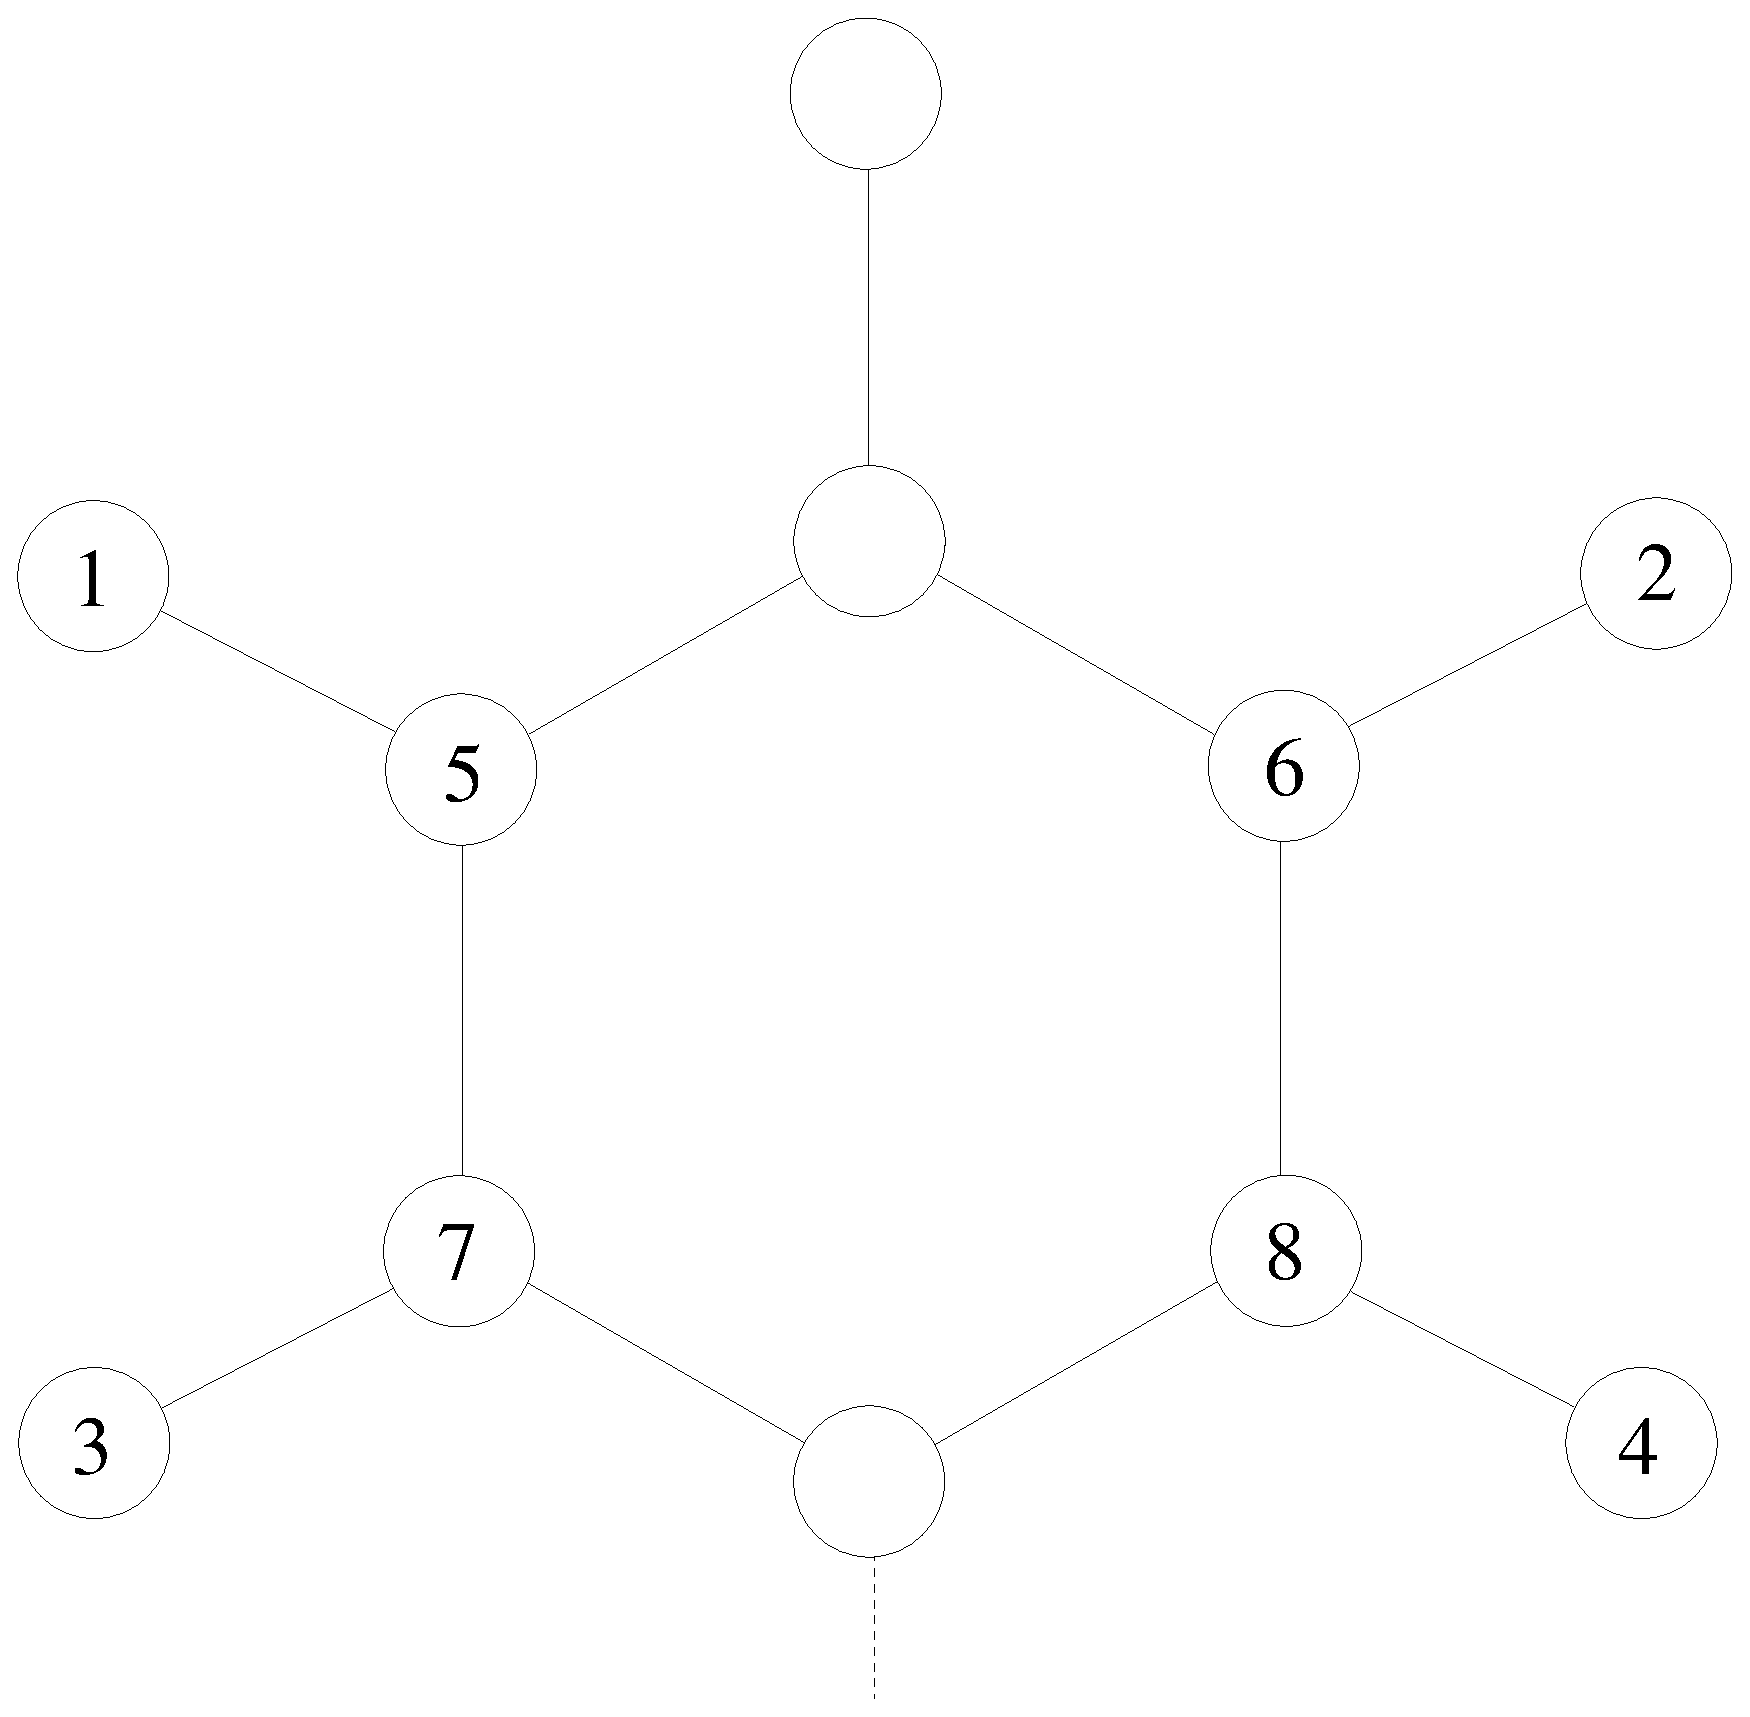
\includegraphics[width=0.5\textwidth]{PHE.eps}}
\end{figure}

For the phenylalanine example illustrated we must allow three other pairs of
atoms to exchange if we swap 7 and 8. Hence a suitable {\tt perm.allow} entry is
{\obeylines
1
2 3
7 8 5 6 1 2 3 4
}
Here $n=2$ and $s=3$: if we exchange 7 and 8 then we must also exchange 5 and 6,
1 and 2, and 3 and 4. There are two atoms in each of the three secondary sets, 
since we have specified 7 and 8 as the two primary atoms.

Here is an example {\tt perm.allow} file for a water trimer using
the flexible {\keyw{QTIP4PF}\/} potential, where the energy is invariant to permutations
of water molecules and to exchanges of hydrogens in the same molecule. However,
hydrogens cannot exchange between different oxygens:
{\obeylines
4
3 2
1 4 7 2 3 5 6 8 9
2 0 
2 3
2 0 
5 6
2 0 
8 9
}
The first group of three oxygens has two atoms that must move with each oxygen,
i.e.~atoms 2 and 3 for oxygen 1, etc. Hydrogen permutations for each oxygen are
allowed by the three following groups. This scheme allows atoms to appear in more 
than one group. There must be a group containing each complete set of permutations
in order for permutation-inversion isomers to be recognised. The format
is compatible with an older scheme, where only pair swaps were allowed for
associated atoms, but now allows for more general permutations.

Scripts to generate allowed permutations automatically for CHARMM and AMBER are available from
the group web site. It is essential to use symmetrised versions of the corresponding
force fields! 


\ksec{PLUS}{\/}: when combined with keywords {\keyw{NEON}\/} or {\keyw{ARGON}\/}
uses a diatomics-in-molecules potential for the singly charged cation.

\ksec{PMAX}{ max\/}: {\it max\/} is the maximum probability of dihedral angle twisting for {\keyw{AMBER}\/}.

\ksec{PMIN}{ min\/}: {\it min\/} is the minimum probability of dihedral angle twisting for {\keyw{AMBER}\/}.

\ksec{POWER}{ ipow\/}: {\it ipow\/} is the initial power for shifts in the old line minimisation routine
for conjugate gradient. LBFGS minimisation should be used instead.

\ksec{PROJI}{\/}: turns on projection operator to enforce $I$ point group symmetry
in {\bf mylbfgs.f}. The geometry is projected after every proposed step.

\ksec{PROJIH}{\/}: turns on projection operator to enforce $I_h$ point group symmetry
in {\bf mylbfgs.f}. The geometry is projected after every proposed step.

\ksec{PTMC}{ histmin histmax ptemin ptemax pttmin pttmax exchprob nequil ptsteps nenrper hbins\/}: 
requests a standard parallel tempering MC run.
This keyword also specifies the energy range for the histogram of quench energies,
{\it histmin\/} to {\it histmax\/},
the energy range for the histogram of instantaneous configurations, {\it ptemin} to {\it ptemax}, 
the temperature range ({\it pttmin} and {\it pttmax}), 
the probability of attempting an exchange {\it exchprob}, the 
number of equilibration steps, {\it nequil},
the number of parallel tempering MC steps without quenching,  {\it ptsteps},
the number of bins for the histogram of instantaneous potential energy, {\it nenrper}, and
the number of bins for the histogram of quench energies, {\it hbins}.
Should be used together with the {\keyw{MPI}\/} keyword. % and {\keyw{BINSTRUCTURES}\/} keywords.
(This option is only available if the source is compiled with an MPI enabled.)  

\ksec{PULL}{ a1 a2 f\/}: apply a static force to the potential, equivalent to adding
the term $V_{\rm pull}=-f(z_{a1}-z_{a2})$. Here $z_{a1}$ and $z_{a2}$ are the $z$
coordinates for atoms $a1$ and $a2$, and $f$ specifies the force.
This potential is designed to simulate a pulling experiment with static force where
a molecule is pulled along the $z$ axis from atoms $a1$ and $a2$.

\ksec{QCUTOFF}{ qcut\/}: {\it qcut\/} is a distance cut-off for Coulomb interactions in {\keyw{AMBER}\/}.

\ksec{QMAX}{ cgmax\/}: {\it cgmax\/} is the tolerance for the 
RMS force in the final set of quenches that are used to produce
the output for file {\tt lowest}. The default is 
{\it cgmax\/}$=10^{-3}$, but the appropriate value depends upon the system in question.
{\it TIGHTCONV} can be used instead.

\ksec{QUAD}{\/}: requires documentation.

\ksec{QUCENTRE}{\/}: sets the centre of coordinates to the origin (0,0,0) before each MC step is taken (so after each quench), but not during the minimisation itself unlike {\keyw{CENTRE}}. 

\subsection{R-S}
\ksec{RADIUS}{ radius\/}: sets the radius of the container that prevents particles
evaporating during quenches. If unset the program calculates an appropriate value
based upon the volume per particle for close-packed material and the known pair
equilibrium distance for the given potential. The formula employed is
$$  RADIUS=r_e\left[1 + \left(3 n \over 4\pi\sqrt{2}\right)^{1/3}\right], $$
where $n$ is the number of atoms and $r_e$ is the pair equilibrium
separation.\cite{kittel76} The `1' in this formula is to allow some extra space for
more open structures.

\ksec{RANDOMSEED}{\/}: specifies that the random number generator should be seeded with system time after each quench, allowing simple parallel use. Currently functional only for the CHARMM and AMBER potentials.

\ksec{RANSEED}{ i\/}: integer seed for the random number generator.

\ksec{RCUTOFF}{ rcut\/}: {\it rcut\/} is a distance cut-off in {\keyw{AMBER}\/}.

\ksec{RESIZE}{ resize\/}: all the coordinates are multiplied by {\it resize\/} after
they have been read in, before any other operations are performed. This command is useful
for scaling results obtained with one potential for a system with a different pair
equilibrium distance.

\ksec{RESTART}{\/ nrelax nhs\/}: reseed runs if a step in not accepted
within twice {\it nrelax} steps.
{\it nhs} is the number of hard sphere moves used to produce the new starting configuration.
If {\it nhs=0} (the default) then the geometry is changed by reseeding.

\ksec{RESTORE}{\/ dumpfile intEdumpfile\/}: restore a previous {\tt GMIN} run from a {\it dumpfile}.
The number of basin-hopping steps performed will be the difference between the number
requested for the run that produced the dumpfile, minus the number that were completed
at the point the dumpfile was created. This option is not available before version 2.3.
If you are using the {\it A9INTE\/} keyword, you can specify the interaction enthalpy
dump file to restore from as a second arguement.

\ksec{RGCL}{2\/}: specifies a DIM rare gas-Cl$_2$ potential.

\ksec{RINGROTSCALE}{ factor\/}: when applying cartesian moves with CHARMM, amino acid rings are moved as rigid units. Setting {\it factor} (default 0.0) between 0.0 and 1.0 will apply a random rotation to these rings during step taking. The suggested value is 0.1 to prevent the regular formation of high energy structures. 

\ksec{RKMIN}{\/}: specifies a Runga-Kutta minimisation scheme. 
Very inefficient.

\ksec{RMS}{ rmslimit rmstol rmssave lca best}: used with {\keyw{CHARMM}} keyword to
specify that the RMSD compared to a reference geometry is calculated. The reference geometry must 
be given in xyz-format in an additional file {\tt compare}. {\it rmssave} is an integer 
that specifies the number of lowest energy geometries and RMSD $\le$ {\it rmslimit}
to save. Geometries are only saved if their RMSD's are more than {\it rmstol} 
different. The flag {\it lca} controls whether the all-atom RMSD ({\it lca}=0) or the $C_{\alpha}$-RMSD 
({\it lca}=1) is calculated. The flag {\it best} determines which structure is compared to the reference
after each quench. {\it best}=0 implies the current quench minimum and {\it best}=1 implies the current best (lowest energy) minimum. If {\keyw{TRACKDATA}} is also specified, the RMSD calculated after each quench is produced in the file `rmsd' in gnuplot readable format.

\ksec{ROTAMER}{ maxchange pselect occuw (centre cutoff)\/}: Used with AMBER9 only. Specifies that rotamer moves should be taken. Every step, up to {\it maxchange} rotamers may be selected with a probability {\it pselect}. {\it occuw} determines the minimum \% occupation a rotamer must have to be selected from the library\cite{lovelljm00} when making a change. For example, {\it occuw} $= 0.004$ restricts possible rotamer choice to those with a greater than 0.4\% occupation. If you want to focus rotamer changes around a ligand/binding pocket, the optional {\it centre} and {\it cutoff} arguements may be used. {\it centre} specifies the residue of interest (for example a ligand), and {\it cutoff} the limiting distance from this centre that rotamers may be changed. The selection probability decreases linearlly from the {\it centre} residue. To use these moves, you need three files found in the SCRIPTS directory: PdbRotamerSearch, penultimate.lib and rotamermove.csh in your working directory for each run. 

\ksec{SAVE}{ nsave\/}: {\it nsave\/} is an integer that specifies the number of lowest
energy geometries to save and summarise in the file {\tt lowest}. 
Arrays are now dynamically allocated, so any positive integer can be specified.

\ksec{SAVEINTE}{ nsaveinte\/}: {\it nsaveinte\/} is an integer that specifies the number of lowest
interaction enthalpy geometries to save and summarise in the file {\tt intelowest}. See {\it A9INTE\/}. 

\ksec{SETCENTRE}{ x y z\/}: Sets the centre of mass/coordinates (before the initial quench) to ({\it x,y,z\/}). For example, {\keyw{SETCENTRE} 0.0 0.0 0.0\/}
would translate the centre of mass to the origin.

\ksec{SC}{ nn mm sig sceps scc\/}: specifies a Sutton-Chen potential\cite{suttonc90} with
parameters $n=${\it nn\/}, $m=${\it mm\/}, $a$={\it sig\/}, $\epsilon=${\it sceps\/} and 
$c=${\it scc\/}.

\ksec{SEED}{ nsstop\/}: if the {\keyw{SEED}\/} keyword appears then the program
looks for a file {\tt seed} containing coordinates, which are used to `seed' the new run.
The number of coordinates given in this file should be no more than one less than the number
given in {\tt coords}. The specified coordinates are frozen from the first step until 
step {\it nsstop\/}.

\ksec{SHIFTCUT}{\/}: specifies a shifted-truncated potential for bulk binary Lennard-Jones.

\ksec{SIDESTEP}{ smax\/}: specifies the maximum step in Cartesian coordinates for side-chains
in {\keyw{AMBER}\/}.

\ksec{SLOPPYCONV}{ bgmax\/}: specifies a basin-hopping run (as opposed to standard MC
on the untransformed surface). {\it bgmax\/} is the convergence criterion
for the RMS force in the basin-hopping
quenches. If this criterion is too strict then the run time will be greatly increased.
If it is too sloppy then the performance of the algorithm is impaired. Different values
are needed for different potentials. {\it BASIN} can be used instead.

\ksec{SORT}{}: for pairwise potentials the atoms can be sorted from most to least
strongly bound. The {\keyw{SORT}} keyword enables this sorting for the coordinates printed
in file {\tt lowest}. This can be useful for seeding subsequent runs by removing the
most weakly bound atoms. This sort is not set by default and is meaningless if the
pair energies are not computed.

\ksec{STAR}{}: specifies an excited state calculation for Ar$^*_n$ or Ne$^*_n$ for
a diatomics-in-molecules potential when used with {\keyw{NEON}\/} or {\keyw{ARGON}\/}.

\ksec{STEP}{ step astep ostep block\/}: specifies the maximum step sizes. {\it step\/} is
for the maximum change of any Cartesian coordinate and {\it astep\/} specifies a tolerance
on the binding energy of individual atoms (if available, i.e.~for Morse and LJ) below
which an angular step is taken for that atom. See the following section for more details.
{\it ostep\/} is the maximum displacement of an axis-angle coordinate for a rigid body system
and {\it block\/} (an integer) is the block size for which separate translational and orientational
displacements will be made for rigid bodies. Omitting {\it block\/} or using a value of zero results in
translational and orientational steps being taken simultaneously
for rigid bodies. The default values for {\it step\/},
{\it astep\/} and {\it ostep\/} are all 0.3 and the default value of {\it nblock\/} is zero.

\ksec{STEEREDMIN}{ smink sminkinc smindiststart smindistfinish sminatoma sminatomb\/}: specified steered 
minimisation should be performed (must be used with {\keyw{AMBER9}}). For a protein/ligand system, this adds a translation
to the MC move. The vector between the centre of coordinates of groups A and B (as defined in the file movableatoms)
is calculated and set to {\it smindiststart}. During the following minimisation, a restoring force is applied to 
the ligand. The harmonic force constant is initially zero, and rises by {\it sminkinc} every LBFGS step up to a
maximum of {\it smink}. The force is applied until the A->B distance is less than {\it smindistfinish}.  

\ksec{STEPS}{ mcsteps tfac\/}: determines the length of the
basin-hopping run through the integer {\it mcsteps\/} and the annealing protocol through
the real variable {\it tfac\/}. The temperature is multiplied by {\it tfac\/}
after every step in each run. 

\ksec{STICKY}{ nrbsites, sigma\/}: specifies a `sticky patch' potential with {\it nrbsites}
sites in the rigid body reference and a value of {\it sigma} for the $\sigma$ parameter.

\ksec{STOCK}{ mu lambda}: specifies a Stockmeyer potential with parameters
$\mu$ and $\lambda$, respectively.

\ksec{STRAND}{}: specifies a system of $\beta$ strands coded using the rigid body formalism.

\ksec{SW}{\/}: specifies the Stillinger-Weber Si potential.

\ksec{SYMMETRISE}{ int tol1 tol2 tol3 tol4 tol5 qmax mdiff d}: specifies that the symmetrisation
routine should be called every {\it int} steps. The five {\it tol} parameters are tolerances
for various parts of the routine: 
{\it tol1} is used in {\bf ptgrp.f} in defining orbits; 
{\it tol2} is the distance tolerance used in {\bf ptgrp.f} to define point group symmetry operations;
{\it tol3} is the maximum relative difference in principal moments of inertia used to
diagnose point groups with degenerate irreducible representations in {\bf ptgrp.f};
{\it tol4} is the distance cutoff used to determine if a symmetry element has been lost in {\bf symmetry.f}.
Since we are dealing with approximate symmetries, this parameter may be larger than {\it tol2}.
It is compared to the largest atomic displacement divided by the corresponding radius
for the closest permutation.
{\it tol4} is also used to test whether atoms lie on a given symmetry element, and in testing 
whether orbits generated from `floaters' are actually contained in the core.
{\it tol5} is generally to check for atom clashes in {\bf symmetry.f}, including analysis of
missing sites in orbits, as well as overlap between orbits generated from `floaters' and
previous core or new orbit sites.
{\it qmax} is the maximum number of quenches allowed for each call to {\bf symmetry.f}.
{\it mdiff} is used to test whether a generated symmetry operation is new. If any of the nine
components of the corresponding $3\times3$ matrix differs by more than {\it mdiff} from an
existing matrix then the operations are considered to be different.
{\it d} is the exponential factor used in constructing a centre of mass that is biased towards
core atoms. The contribution of each atom is weighted by $\exp(-dx(i))$, where $x$ is the 
centre of mass distance of atom $i$ on the previous cycle.

\subsection{T-Z}
\ksec{TABOO}{ nlist\/}: specifies a taboo list of the {\it nlist\/} lowest minima should be maintained.

\ksec{TARGET}{ target1 target2 $\cdots$\/}: specifies any number of target energies. 
The current run stops in an orderly
fashion if the current quench energy is within {\it econv\/} of any target (see {\keyw{EDIFF}\/}).

\ksec{TEMPERATURE}{ temp\/}: defines the temperature, {\it temp\/}, at which the 
MC runs are conducted. Different values can be specified for serial `parallel' runs if
{\keyw{PARALLEL}} is set.
For true parallel basin-hopping use the {\keyw{BHPT}\/} keyword and omit {\keyw{TEMPERATURE}\/}.

\ksec{TETHER}{ hdistconstraint hwindows ExtrapolationPercent lnHarmFreq}: requests a calculation of the vibrational density of
states for a given minimum. {\it hdistconstraint} is the minimised average radius of the basin of attraction to which the minimum
belongs, {\it hwindows} is the number of potential energy windows into which a WL simulation is split. {\it 
ExtrapolationPercent} is the percentage of the whole potential energy spectrum, for which the density of states is estimated from
the harmonic approximation and not sampled. {\it lnHarmFreq} the log product of positive Hessian
eigenvalues.

\ksec{THOMSON}{ q\/}: specify the Thomson problem for unit charges on a sphere.
If {\it q\/} is present it is taken to be the charge on one particle, which can
therefore be different from all the other unit charges and is read as a real number.

% Doesn't appear to be coded?
% \ksec{THRESHOLD}{ \/}: specifies threshold acceptance of steps. The change in potential energy must be
% less than the value of the {\keyw{TEMPERATURE}\/} variable for a step to be accepted.

\ksec{TIGHTCONV}{ cgmax\/}: cgmax is the tolerance for the
RMS force in the final set of quenches that are used to produce
the output for file {\tt lowest}. The default is
{\it cgmax\/}$=10^{-3}$, but the appropriate values depend upon the system in question.
{\it QMAX} can be used instead.

\ksec{TIP}{ n\/}: specifies a TIP{\it n\/}P intermolecular potential for rigid body water molecules.
$\ \le n \le 5$.

\ksec{TOLBRENT}{ tolb\/}: parameter for {\keyw{DBRENT}\/} minimisation. 
Inefficient compared to LBFGS.

\ksec{TOMEGA}{}: used with the {\keyw{CHARMM}} keyword to specify that peptide bonds will be twisted along with all other dihedrals.

% \ksec{TN}{\/}: specifies a truncated Newton minimisation scheme. 
% Inefficient compared to LBFGS.

\ksec{TOSI}{ app amm apm rho\/}: specifies the Tosi-Fumi potential\cite{tosif64}
with parameters $A_{++}$, $A_{--}$, $A_{+-}$ and $\rho$.

\ksec{TRACKDATA}{}: produces `energy.dat' and `markov.dat' containing the quench number and 
associated energy and markov energy in two columns and `best.dat', containing the current quench number and the current lowest
total energy. If {\keyw{RMS}\/} is also specified, a file called `rmsd.dat' is produced containing the RMSD from a reference structure.
See {\keyw{RMS}\/} for more information. This allows plotting with gnuplot to monitor convergence of multiple runs.
If {\it A9INTE} is also specified, two additional output files are produced, `intE.dat' containing the quench number and associated interaction
enthalpy, and `bestintE.dat' containing the quench number and current lowest interaction enthalpy. This keyword does not yet function for MPI runs.

\ksec{TSALLIS}{ q\/}: specifies that steps are accepted/rejected using Tsallis statistics with the
given value of {\it q\/}, rather than the usual Boltzmann condition.

\ksec{TWOPLUS}{\/}: when combined with keywords {\keyw{NEON}\/} or {\keyw{ARGON}\/}
uses a diatomics-in-molecules potential for the doubly charged cation.

\ksec{UACHIRAL}{\/}: MUST be included when using ff03ua, the AMBER united atom forcefield unless you have disabled the checks for inverted chiral carbons
 with {\keyw{NOCHIRALCHECKS}\/}. {\keyw{UACHIRAL}\/} ensures the correct impropers are used to define sidechain chirality when HB hydrogen is missing. 

\ksec{UPDATES}{ nup\/}: {\keyw{UPDATES}\/} is the number of previous steps saved in the LBFGS routine,
default 4.

\ksec{VGW}{ ljsigma ljepsilon taumaxsg taumaxfg}: Specifies use of VGW quantum quenching in place of
classical minimization routines such as LBFGS. {\it ljsigma} and {\it ljepsilon} are the corresponding Lennard-Jones
parameters that must be specified, and taumaxsg and taumaxfg are the maximum value of ``imaginary'' time $\tau$ (inverse tempertaure) for the propagation.
The former pertains to the faster ``single-particle'' SP-VGW used for quenching during the MC runs, and the latter for the more accurate
``fully-coupled'' VGW used for the final quenching (analogous to the tight convergence of the LBFGS). A $\tau$ of at least
2.5 is recommended for the SP-VGW and 5.0 for the FC-VGW. A file {\it vgwdata} containing the masses (in a.m.u.) of all particles, in order of the location
of their {\it xyz} coordinates in ``{\it coords}'' must be present (e.g. for a 38 atom Ne cluster, {\it vgwdata} will have 38 lines of ``{\it 20}''). Different
masses are permitted, though the current version allows for only one set of LJ parameters. 

\ksec{VGWCPS}{ on magnitude}: Specifies use of contraining potential for SP-VGW (sloppy convergence), as clusters expand during quantum quenching
with decreasing mass. 1 or 0 for {\it on} corresponds to on/off,
and magnitude should range from 1 to 1000, with 1 having minimal effect, 1000 being highly constrained. Default value is ``on'', with magnitude 1.

\ksec{VGWCPF}{ on magnitude}: Same as VGWCPS but for FC-VGW, used for the final, full quenching (tight convergence).

\ksec{VGWTOL}{ magnitude}: Absolute tolerance parameter for differential equation solver used for VGW quenching. Default value is 0.0001.
For highly quantum or ``stiff'' systems this may need to be increased, while it may be decreased for ``softer'' or less quantum systems to enhance
speed.
 
\ksec{VISITPROP}{}: if specified the Wang-Landau convergence is governed by proportionality of visits to the current value of
the modification factor, and not the histogram flatness criterion \cite{ZhouB03}.

\ksec{WELCH}{ $A_{++}\ A_{--}\ A_{+-}\ \rho\ Q_+\ Q_-\ \alpha_+\ \alpha_-$\/}: specifies a Welch binary
salt potential with the parameters indicated.

\ksec{ZETT}{1\/} and {\keyw{ZETT2}\/}: specify the Zetterling potentials.
% </kwd>

\section{Angular Steps}

For pure pair potentials the total energy can be broken down into a sum of binding
energies for the individual atoms. This is coded for the Morse and LJ potentials.
If the binding energy of any atom is lower than that of the most tightly bound atom
multiplied by the variable {\it astep\/} (see the {\keyw{STEP}\/} command above) then
that atom is randomly replaced on the sphere of radius equal to that of the atom furthest
from the centre of mass. Hence if {\it astep\/} is zero angular steps will never be taken,
and the closer this parameter is to one the more atoms will undergo such displacements.
If the step sizes are adjusted to give the required acceptance ratio then both {\it step\/} and
{\it astep\/} are multiplied or divided by $1.05$ every {\it naccept\/} steps depending
upon the current acceptance ratio. If {\keyw{FIXSTEP}\/} has been specified then the temperature
is adjusted in the same way and {\it step\/} and {\it astep\/} are unchanged.

% <systems>
\section{Some Recognised Systems}

\subsection{AMBER}

Specifies the AMBER force field. Coordinates are read from file {\tt coords.amber}.
See also associated keywords {\keyw{PMAX}\/}, {\keyw{PMIN}\/}, {\keyw{NMAX}\/}, {\keyw{NMIN}\/},
{\keyw{SIDESTEP}\/}, {\keyw{RCUTOFF}\/}, {\keyw{QCUTOFF}\/} and {\keyw{FAKEWATER}\/}.

\subsection{Binary Lennard-Jones}

If the {\keyw{BINARY}\/} keyword is specified then a binary Lennard-Jones
potential is used\cite{sastryds98}. {\keyw{PERIODIC}\/} must also be
specified. Reduced units are used with $\epsilon_{\rm AA}=\sigma_{AA}=1$.
{\keyw{BLJCLUSTER}\/} specifies a binary Lennard-Jones cluster.

\subsection{BLN Off-Lattice Protein Model}
\label{sec:BLN}

The general three-colour bead protein model is specified by keyword {\keyw{BLN}}.
The potential follows the form described in
{\it Proc.~Natl.~Acad.~Sci.~USA}, {\bf 100}, 10712, 2003, expect that
the coefficients $A_i$, $B_i$, $C_i$ and $D_i$ include a factor of $\epsilon$
explicitly.

{\arraycolsep0pt\begin{eqnarray}
V&\,=\,&\frac{1}{2} K_r\sum_{i=1}^{N-1}(R_{i,i+1}-R_{\rm e})^2
 +\frac{1}{2} K_\theta\sum_i^{N-2}(\theta_i-\theta_{\rm e})^2 \nonumber\\
 &&+\,\epsilon\sum_i^{N-3}\Big[A_i(1+\cos\varphi_i)+B_i(1-\cos\varphi_i) \nonumber\\
  && \qquad +C_i(1+\cos3\varphi_i)+D_i\left(1+\cos\left[\varphi_i+\pi/4\right]\right)\Big] \nonumber\\
 &&+\,4\epsilon\sum_{i=1}^{N-2}\sum_{j=i+2}^N \left[S_{12}\left(\frac{\sigma}{R_{ij}}\right)^{\!12}
    +S_6\!\left(\frac{\sigma}{R_{ij}}\right)^{\!6}\right],
\label{barrelpot}
\end{eqnarray}}
\noindent where $R_{ij}$ is the separation between beads $i$ and $j$ and
the units of distance and energy are $\sigma$ and $\epsilon$, respectively.
The first term represents the bonds linking successive beads in the linear chain, and a 
value of $K_r=231.2\,\epsilon\sigma^{-2}$ was used in most of the work on the 
Honeycutt and Thirumalai frustrated 46-bead model.
The second term is a sum over the bond angles, $\theta_i$, defined by the triplets
of atomic positions ${\bf R}_i$ to ${\bf R}_{i+2}$, and values
$K_\theta=20\,\epsilon\,{\rm rad}^{-2}$ and $\theta_{\rm e}=105^\circ$ were
used for the 46-bead model.
The third term
is a sum over the dihedral angles, $\varphi_i$, defined by the quartets ${\bf R}_i$ to
${\bf R}_{i+3}$. 
In the 46-bead model $A_i=C_i=1.2$ if the quartet involved no more than one N monomer, generating
a preference for the {\it trans\/} conformation ($\varphi_i=180^\circ$), whereas if two or three
N monomers are involved then $A_i=0$ and $C_i=0.2$.
This choice makes the three neutral
segments of the chain flexible and enables them to accommodate turns.
A general specification of these parameters is possible in the new BLN framework
via the auxiliary file {\tt BLNsequence}.
The last term in (\ref{barrelpot}) represents the nonbonded interactions.
In the current BLN implementation $R_{\rm e}$ is set equal to $\sigma$, i.e.~to 
unity in reduced units.

An appropriate {\tt BLNsequence} file for the usual 46-bead model contains the following
lines:

{\obeylines
\noindent comment: $S_{12}>0$ and $S_6<0$ for B-B, L-L and L-B, N-L and N-B and N-N
\noindent 1.0D0 -1.0D0
\noindent 0.33333333333333D0 0.33333333333333D0
\noindent 1.0D0 0.0D0
\noindent comment: coefficients A, B, C, D
\noindent comment: for Helical, Extended and Turn residues in order, four per line
\noindent 0.0D0 1.2D0 1.2D0 1.2D0
\noindent 0.9D0 0.0D0 1.2D0 0.0D0
\noindent 0.0D0 0.0D0 0.2D0 0.0D0
\noindent LBLBLBLBBNNNBBBLBLBBBNNNLLBLLBBLLBNBLBLBLBLNNNLBBLBLBBBL
\noindent EEEEEETEHTHEEEEEEEEHHEHHHHHHHHHHEHTEEEEEEETTTEEEEEEEE
}

\noindent The penultimate line defines the sequence, and the final line
defines which set of $A_i$, $B_i$, $C_i$ and $D_i$ parameters apply to which 
parts of the structure.\cite{BrownFH03}


\subsection{Diatomics-in-Molecules}

At present diatomics-in-molecules (DIM) potentials are available for various
clusters, which are specified by the line {\keyw{ARGON}\/}, {\keyw{NEON}\/},
{\keyw{ARNO}} or {\keyw{RGCL2}\/} in {\tt data}.
Further keywords specify the precise nature of the system for argon or
neon clusters: {\it NEUTRAL\/} for ground state neutral
clusters, {\keyw{PLUS}\/} for a single positive charge, {\keyw{TWOPLUS}\/} for a double positive
charge, {\keyw{STAR}\/} for an electronic excited state and {\keyw{DIPOLES}\/} for the first order
induction energy in a charged system. Rare gas-Cl$_2$ and Ar$_N$-NO DIM potentials
are specified by the {\keyw{RGCL2}\/} keyword.

\subsection{DFT-based tight-binding}

If the {\keyw{DFTB}\/} keyword is specified then a DFT-based tight-binding potential
is used. See also the {\keyw{MULTIPLICITY}\/} keyword.

\subsection{LB2}

This keyword specifies the potential\cite{LB299a,LB299b,LB204}
\begin{equation}
V = \frac{\epsilon}{2} \sum_{i<j} \left[ \left(\frac{r_{ij}}{\sigma}\right)^2+
\left(\frac{\sigma}{r_{ij}}\right)^2\right],
\end{equation}
where $\epsilon$ and $\sigma$ are set to unity.

\subsection{Farkas}

The Farkas potentials for aluminium and nickel are specified by keywords {\keyw{FAL}\/} and
{\keyw{FNI}\/}, respectively.

\subsection{Lennard-Jones}

This is the default potential if nothing is specified in {\tt data}. Reduced units are
assumed with $\epsilon=\sigma=1$.

\subsection{Morse}

This potential is specified by the line {\keyw{MORSE} rho\/} in {\tt data} and gives a
a Morse potential with $D=r_e=1$. 
The remaining range parameter,\cite{braierbw90,doyewb95,doyew96a} $\rho$, has a default 
value of six.

\subsection{P46}

Keyword {\keyw{P46}\/} specifies a 46-bead three-colour model polypeptide. 
See also the more general implementation of the BLN model in \S \ref{sec:BLN}.

\subsection{Stillinger-Weber Si}

Specified by the keyword {\keyw{SW}\/}.

\subsection{Sutton-Chen}

These potentials\cite{suttonc90} are specified by the line {\keyw{SC} nn mm sig sceps scc\/} in {\tt data},
as described above. 

\subsection{Tight-binding}

Tight-binding potentials for silicon are specified by the keywords {\keyw{MSORIG}\/} 
and {\keyw{FRAUSI}\/}.
These potentials also understand the 
keywords {\keyw{PERIODIC}\/} and {\keyw{CUTOFF}\/} which enable calculations on bulk material
to be performed and a cutoff to be imposed on either cluster or bulk calculations.
Keyword {\keyw{ANGSTROM}\/} specifies coordinates in \AA ngstrom rather than bohr.

\subsection{TIP{\it n\/}P Water}

The TIP{\it n\/}P intermolecular water potentials are specified by the keyword {\keyw{TIP}\/}.
{\it n\/}=1 through 5 are currently coded. For $N$ water molecules the first $N$ lines of
the {\tt coords} file are the coordinates of a reference origin in each of $N$ rigid molecules,
and the next $N$ lines are angle-axis coordinates. The same convention is used in the output
file {\tt lowest}. The lowest minima are also dumped in xyz format in the file {\tt tip.xyz}.

\subsection{Tosi-Fumi}
 
Keyword {\keyw{TOSI}\/} specifies a Born-Mayer potential of the form
$$ E = \sum_{i<j}\left[ {q_i q_j\over r_{ij}} + A_{ij}\exp(-r_{ij}/\rho) \right]. $$
The sum runs over all ions. Tosi-Fumi\cite{tosif64} parameters in atomic units should be
entered after the Tosi keyword in the order $A_{++}$, $A_{--}$, $A_{+-}$, $\rho$.
The ions are specified in file {\tt coords} using PL and MI for plus and minus, respectively,
and can be in any order. There need not be equal numbers of positive and negative ions.
Note that the Welch potential has been fitted to include ion polarizabilities and is described below.

\subsection{Welch}This keyword specifies a Welch potential\cite{welchld76,phillipscb91} of the form
\begin{eqnarray*}
% I have tried \bm \boldsymbol etc. but I can't get a bold mu?!
E &= \sum_{i<j}\Bigg[ {\D q_i q_j\over\D  r_{ij}} + A_{ij}\exp(-r_{ij}^{\rm eff}/\rho)
              -{\D q_i({\boldsymbol \mu}_j\cdot{\bf r}_{ij})\over\D  r_{ij}^3}
              -{\D q_j({\boldsymbol \mu}_i\cdot{\bf r}_{ji})\over\D  r_{ij}^3} \\
             &-3{\D   ({\boldsymbol \mu}_i\cdot{\bf r}_{ij})
                   ({\boldsymbol \mu}_j\cdot{\bf r}_{ij})\over\D  r_{ij}^5}
              +{\D  {\boldsymbol \mu}_i\cdot{{\bf{\mu}}}_j\over\D  r_{ij}^3}\Bigg]
              +\sum_i {\D \mu_i^2\over\D 2\alpha_i}, \\
\end{eqnarray*}
where
$$ {\bf r}_{ij}^{\rm eff}={\bf r}_{ij}+{{\boldsymbol \mu}_i\over Q_i}-{{\boldsymbol \mu}_j\over Q_j},
    \qquad r_{ij}^{\rm eff}=\left|{\bf r}_{ij}^{\rm eff}\right|. $$
Welch parameters in atomic units should be
entered after the Welch keyword in the order $A_{++}$, $A_{--}$, $A_{+-}$, $\rho$, $Q_+$,
$Q_-$, $\alpha_+$, $\alpha_-$.
The ions are specified in {\tt coords}  using atom types PL and MI for plus and minus, respectively,
and can be in any order. There need not be equal numbers of positive and negative ions.

% </systems>

% <examples>

\section{Example {\tt data} Files}

A basin-hopping run of 10,000 MC steps at reduced temperature $0.8$ for the Lennard-Jones potential
with a constant temperature specified by the `1.0' on the {\keyw{STEP}S\/} line.
Seeding occurs for the first 100 steps, so a file {\tt seed} is required in the 
working directory. The final quenches to produce the output in {\tt lowest} are much
tighter than the relatively `sloppy' quenches for the basin-hopping run (compare the
{\it SLOPPYCONV\/} line with the {\it TIGHTCONV\/} line). The maximum number of iterations per
conjugate gradient step is 250 for the sloppy quenches and 500 for the tight quenches.
The initial linear and angular step parameters are 0.36 and 0.4, and these are adjusted
every 50 steps to try and achieve an acceptance ratio of 0.5.

\medskip
\begin{tabular}{ll}
SLOPPYCONV & 0.01 \\
TIGHTCONV & 1.0D-3 \\
SORT \\
MAXIT & 250 500 \\
STEPS & 10000 1.0 \\
STEP & 0.36 0.4 \\
TEMPERATURE & 0.8 \\
\end{tabular}
\medskip

\noindent The next example is similar to the above but employs parameters that seem
to be suitable for a Morse potential with $\rho=6$.

\medskip
\begin{tabular}{ll}
SLOPPYCONV & 0.01 \\
TIGHTCONV & 1.0D-3 \\
SORT \\
EDIFF & 0.01\\
MORSE & 6.0\\
MAXIT & 200 500\\
STEPS & 10000 1.0\\
STEP & 0.35 0.4\\
TEMPERATURE & 0.6\\
\end{tabular}
\medskip

\noindent Global optimisation for a water cluster using the TIP4P potential.
The initial step sizes for translational and orientational rigid-body coordinates are
0.6 and 0.9, respectively, and the block size for separate translational and orientational
steps is 200.

\medskip
\begin{tabular}{ll}
SLOPPYCONV & 0.01 \\
TIGHTCONV & 0.0001 \\
TIP & 4 \\
CENTRE & \\
MAXIT & 1000 1000\\
STEPS & 50000 1.0\\
STEP & 0.6 0.0 0.9 200 \\
TEMPERATURE & 5.0\\
\end{tabular}
\medskip

\noindent The following input file specifies a basin-sampling run to calculate the density of states for 
a LJ$_{13}$ cluster. The system is
confined to a spherical container of radius $1.8\,\sigma$, 
the geometry will be perturbed by $0.2\,\sigma$ at each step with no
angular steps allowed. The run will terminate after $1000000$ 
MC steps or when the WL convergence criterion {\it targetwl}
is satisfied, whichever is the earliest. Setting the temperature to zero indicates that 
a Wang-Landau type MC is used instead of
a conventional temperature-dependent MC run. In keyword {\it HISTOGRAM\/}
the energy of the global minimum of LJ$_{13}$ $-44.3268\,\epsilon$ is chosen
as the energy of the lowest bin {\it histmin}, the energy spectrum above that point is 
separated into $50$ bins of width $0.25$ each. The
starting modification factor and target number of WL iterations are 
{\it histfac} =$ 1.01$ and {\it targetwl} =$ 10$. A square root function
will  be used for decreasing the modification factor upon completion of each WL iteration, 
and the convergence schedule is regulated by {\keyw{VISITPROP}}.  


\medskip
\begin{tabular}{ll}
SLOPPYCONV & 0.001 \\
TIGHTCONV & 1.0D-3 \\
MAXBFGS &  0.1 \\
EDIFF & 0.003 \\
RADIUS &  1.8 \\
MAXIT & 1000 500 \\
STEPS & 1000000 1.0 \\
STEP  & 0.2 0.0 \\
TEMPERATURE & 0.0 \\
HISTOGRAM & -44.3268014195 $\:$ 0.2 $\:$ 1.1D0 $\:$ 50 $\:$ 0.5 $\:$ 10 $\:$ 0.2 \\
EQUILIBRATION 1 100 \\
FIXBOTH \\
BINSTRUCTURES 1 \\
VISITPROP \\
\end{tabular}
\medskip

% </examples>
% <end>
\section{Summary of Major Changes}

\subsection{12/10/10}
Changed to a more flexible scheme for atoms that must move together when
{\keyw{PERMDIST}\/} is pecified, in line with OPTIM and PATHSAMPLE.

\subsection{2/11/07}
Implementation of minimum image convention in distance minimisation.
{\keyw{PERMDIST}} keyword now made consistent with OPTIM and PATHSAMPLE
using {\tt perm.allow} file.

\subsection{31/12/06}
GMIN.2.3 introduced with MPI support by Tetyana Bogdan and David Wales.
New parallel tempering basin-sampling and
parallel tempering basin-hopping algorithms implemented.

\subsection{18/2/05}
\begin{itemize}
\item GMIN.2.0 recoded in fortran90 by Tetyana Bogdan and DJW. All arrays are now dynamically allocated.
\item Basin-sampling procedure programmed by DJW and developed by Tetyana Bogdan. See the new
{\it HISTOGRAM} keyword.
\item Interface to CHARMM added by David Evans and DJW. See keyword {\keyw{CHARMM}} and its associated 
parameters. Internal coordinate minimisation (written by David Evans and developed by Joanne Carr) 
is specified by keyword {\keyw{INTMIN}}.
\item Exploitation of approximate symmetry introduced through {\it SYMMETRY} keyword.
\item Bipartite matching implemented for matching closest permutational isomers
(thanks to Tomas Oppelstrup). Now used with 
the {\keyw{PERMDIST}} keyword, as well as the new taboo-type procedure introduced through keyword {\keyw{AVOID}}.
\item Cooperative moves introduced via keyword {\keyw{COOPMOVE}}.
\item Various new potentials have been added: {\keyw{NATB}} specifies a tight-binding potential
for sodium (can be guided by {\keyw{GUPTA} 21}); various Gupta potentials; Stockmeyer; sticky patches, etc.
\end{itemize}

\subsection{22/6/03}
\begin{itemize}
\item Support for rigid bodies added, e.g.~potentials {\keyw{TIP}\/}, {\keyw{CAPSID}\/} and {\keyw{OTP}\/}.
The centre-of-mass and angle-axis derivatives are calculated in subroutine {\tt rigidfunc.f}, so for pairwise
site-site potentials all that is needed are additional statement functions for these potentials and their
first derivative with respect to the distance.
\item Guiding potentials changed. The new keyword {\keyw{GUIDE}\/} allows specification of a parameter,
{\it guidecut\/}, the RMS force below which the real potential is used. 
\item Glue potential for lead added.
\item Keyword {\keyw{TSALLIS}\/} introduced for an alternative to the Metropolis
accept/reject step with Boltzmann statistics.
\item Keywords {\keyw{BINARY}\/}, {\keyw{BLJCLUSTER}\/} and {\keyw{SHIFTCUT}\/} introduced for binary LJ systems,
{\keyw{ZETT1}\/} and {\keyw{ZETT2}\/} for Zetterling potentials, {\keyw{FAL}\/} and {\keyw{FNI}\/} for Farkas Al and Ni
potentials, {\keyw{ARNO}\/}, {\keyw{MULTIPLICITY}\/} for {\keyw{DFTB}\/} and 
{\keyw{AXTELL}\/} for an additive Axilrod-Teller contribution.
Keywords {\keyw{NEWJUMP}\/} and {\it PNEWJUMP\/} for parallel runs with parallel tempering-like jumps
and {\keyw{JUMPMOVE}\/} for jump-walking parallel runs.
Keyword {\keyw{TABOO}\/} for runs with a taboo list.
\item Keyword {\keyw{PERMDIST}\/} added for runs that minimise the distance between two structures by permuting
atoms.

\end{itemize}

\subsection{15/10/99}
\begin{itemize}
\item Replaced conjugate gradient minimisation by the limited memory algorithm
      of Jorge Nocedal\cite{lbfgs}.
\item The convergence for {\it SLOPPYCONV\/} and {\it TIGHTCONV\/} is now
      based only on the RMS gradient. The energy change condition has gone.
\item New parameters for the LBFGS routine. {\keyw{PRINT}LEVEL\/} sets the 
      print level parameters, {\keyw{UPDATES}\/} the number of LBFGS updates
      before resetting and {\keyw{GT}OL\/} the tolerance for line minimisation.
\end{itemize}

\chapter{OPTIM}
\renewcommand{\pname}{OPTIM}

\section{Introduction}
\label{sec:intro}

{\tt OPTIM} is the program for 
locating stationary points on potential energy 
surfaces and calculating reaction pathways. \cite{Wales03}

It's latest version is 4.0.

A number of changes have been introduced from OPTIM.2.3.
In particular, it is no longer necessary to recompile the program to treat larger systems, since
the dynamic memory features of fortran90 have now been used throughout.

The default build target for the Makefile is OPTIM, but three other targets are now
possible, namely COPTIM, UNOPTIM, AMOPTIM, and AMB9OPTIM, which produce corresponding executables interfaced 
to the CHARMM,\cite{mackerellbbdeffgghjkklmmnnprrsssswwyk98,lazaridisk99}
UNRES, AMBER95\cite{cornellcbgmfsfck95} and AMBER 9 potentials, respectively.

Separate directories containing libraries built from modified CHARMM, UNRES and AMBER 9 sources must 
be present to build the corresponding COPTIM, UNOPTIM and AMB9OPTIM executables.

The optimisation algorithms include:
\begin{itemize}
  \item eigenvector-following,
\cite{pancir74,cerjanm81,simonsjto83,onealts84,banerjeeass85,baker86,baker87};
\item steepest-descent (Page-McIver second order; Bulirsch-Stoer, Runga-Kutta, or 
Barzilai-Borwein-Raydan\cite{BB-IMAJNA-1988,Raydan-SIAMJO-1997} for first order);
\item conjugate gradient and hybrids thereof.
\end{itemize}

Pathways can be calculated in several ways, and it is also possible to
use a "fictitious" kinetic metric,
usually referred to as "mass-weighted" coordinates.
There is provision to treat rigid body systems; the
TIPS family of rigid molecule, effective pair potentials for H$_2$O are known to
the program and employ centre-of-mass and Euler angle coordinates. An older
version of the eigenvector-following optimiser is present in the ORIENT3 program, which can treat 
arbitrary mixtures of atoms and rigid molecules using distributed multipoles to
describe the electrostatic energy.\cite{stone81,stonea85}\

These optimisation algorithms can also be
very effective in solving fitting problems, especially if analytic derivatives 
can be obtained.

The main new keywords that were introduced in
OPTIM.3.0 are \keyw{NEWCONNECT} and \keyw{NEWNEB};
the {\keyw{CONNECT}} and \keyw{NEB} keywords remain available, but the new algorithms
will probably be more effective. The \keyw{NEWNEB} keyword specifies a
doubly-nudged elastic band (DNEB) algorithm for double-ended searches,\cite{TrygubenkoW04}
while \keyw{NEWCONNECT} provides a more sophisticated way to link local minima
that are likely to be connected by pathways involving a number of transition states.
The \keyw{GROWSTRING} and \keyw{EVOLVESTRING} keywords provide implementations of the
growing string and evolving string methods.\cite{ERV02,PetersHBC04}
A new framework has also been introduced for treating rigid bodies that interact
via isotropic site-site potentials using angle/axis coordinates.\cite{Wales05}

Also new from OPTIM.3.0 onwards is the ability to specify a file extension when OPTIM is invoked on the
command line. For example, running 
{\obeylines {\tt OPTIM} \qquad 2 \qquad $>$\& }
\noindent will result in all other output files having the 
extension `.2', e.g.~{\tt odata.new.2, points.final.2, output.2 } etc.
In contrast to the use of the {\keyw{FILTH}} keyword, when OPTIM is invoked in this way
it will also assume that all input files carry the same extension, e.g.~{\tt odata.2, finish.2}.
The intention is to retire the {\keyw{FILTH}} keyword as soon as the Filthy\_Phyllis program
has been rewritten appropriately. It will then be possible to use non-integer file extensions;
at the moment only integers between 1 and 999 can be handled.

The OPTIM program has analytic first and second energy derivatives coded for dozens of
empirical potentials and can also read derivatives from disc so that it can be run
iteratively in tandem with {\it ab initio\/} or other packages. 
The only file that you need to start simple calculations is {\tt odata}. 
Each call to OPTIM performs one or more steps of various kinds.
The updated coordinates after every step are saved in order
in file {\tt points}. The coordinates after the final step are also written to file
{\tt points.final} and a new input file for OPTIM based upon this geometry is written
to {\tt odata.new}. This file also contains the energy for the last step and
the point group (if it was evaluated) as \keyw{COMMENT} statements.


\section{Building}

\section{Source code}

OPTIM source code is located in OPTIM/source/ subdirectory. The following files
are responsible for building: Makefile build.csh

\section{The {\tt odata} file}
\label{sec:odata}
\hypertarget{odata}
Input is keyword driven.
The last keyword will usually be \keyw{POINTS}, after which 
the starting geometry is specified, one atom per line, by the atomic symbol (case
insensitive) and the corresponding $x$, $y$ and $z$ coordinates. For potentials that
are coded within OPTIM there will always be an assumed unit system.
OPTIM usually determines the potential to be used from the atomic
symbol of the last atom, and various symbols have evolved for different systems, as
described in \S\ref{sec:potentials}. Free format may be used within each line. Blank lines are ignored,
but there {\bf must not} be any blank lines after the \keyw{POINTS} keyword.
The maximum line length permitted has now been increased to 132 characters.

\section{Keywords}
\label{sec:keywords}
\label{sect:keywords}

The following keywords are recognised, where {\it n\/}, {\it x\/} and {\it exec\/} are integer,
real and character data, respectively.
\smallskip
% </intro>
% <kwd>
%\begin{itemize}
\ksec{2D}: restrict the system to the $x-y$ plane.
\subsection{A}

\ksec{ACE}{ n}: for use with CHARMM runs that employ the ACE implicit solvent model. 
{\it n} specifies the number of calls to the CHARMM energy and gradient for which lists
are held fixed. The default value of {\it n} is 50. 
Note: {\keyw{ENDNUMHESS}} must be used with the ACE solvent model. 
Otherwise {\tt OPTIM} will attempt to use incorrect second derivatives.
{\keyw{ENDNUMHESS}} will be needed in the {\tt odata.start}, {\tt odata.finish}
and {\tt odata.connect} files. 
For {\tt odata.start} and {\tt odata.finish} the keyword {\keyw{ENDHESS}}
must also be included.

\ksec{A}{Ackland id\/}: specifies an Ackland embedded atom metal potential% \cite{} 
coded by Dr Mihai-Cosmin Marinica.
{\it id} specifies the particular metal: 1 is ?, 2 is ?, 3 is ?, 4 is ?, 5 is iron, 6 is a different iron,
7 is tungsten.
Positive values for {\it id} specify periodic boundary conditions, where box lengths must be
specified by the {\keyw{PERIODIC}\/} keyword. 
% Negative values for {\it id\/} specify a cluster calculation. A {\keyw{CUTOFF}\/} value can also
% be used for clusters.

\ksec{ADM}{ n}: will cause the
interatomic distance matrix to be printed every {\it n\/} cycles;
the default for {\it n\/} is 20. This matrix is not printed by default.

\ksec{ALPHA}{}: sets exponent value for averaged Gaussian and Morse potentials,
default value is 6.

\ksec{ALLPOINTS}{}: turns on printing of coordinates to file {\tt points} for
all intermediate configurations. Default is false.

\ksec{AMBER}{}: specifies a calculation with the AMBER potential. This requires
      auxiliary files {\tt amber.dat} and {\tt coords.amber} in the same directory.

\ksec{AMBER}{9 inpcrd inpcrdformat\/}: specifies a calculation with the interfaced 
version of the Amber 9 program package. From this package the Amber force fields 
are being used, with small modifications ({\it e.g.} smooth cut-offs). 
Starting coordinates do not need to be specified in the {\tt odata} file, they
are read from {\it inpcrd} instead (default {\it coords.inpcrd}), in Amber inpcrd 
file format specified by the second optional argument {\it inpcrdformat}.
If the second argument is missing, it is assumed that {\it inpcrd} contains
only three columns with the xyz coordinates of all atoms, in the same order 
as in the topology file. To start a run with this interface, 
several auxiliary files are required in the same directory: input coordinate file
{\it coords.inpcrd}, parameter topology file {\it coords.prmtop}, 
input file to Amber containing force field specifications {\it min.in}, and, if 
desired, a coordinate file different from {\it coords.inpcrd} containing 
starting coordinates.
To turn on smooth cutoffs for the Generalised Born force fields, the keyword 
{\it ifswitch=1} has to be used in the {\it \&cntrl} namelist block of {\it min.in}.
When using the {\keyw{AMBER}9} keyword, any calculated second derivatives will be 
numerical. If one wants analytical second derivatives, the {\keyw{NAB}} keyword 
should be used instead, with the same syntax. The NAB interface does not 
currently support smooth cutoffs, so analytical second derivatives are only 
recommended for stationary points calculated with large cutoffs.
Additional keywords for the AMBER 9 runs are {\keyw{NAB}} and {\keyw{DUMP}STRUCTURES}.

\ksec{AMBERIC}{}: interpolation in bhinterp with internal coordinates. If BACKBONE specified additionally (AMBERIC BACKBONE) the protein backbone is also interpolated in internals. Does not work for polymers.

\ksec{AMBERSTEP}{}: perturbation/twisting in bhinterp done with internal coordinates

\ksec{AMBPERTONLY}{ n}:only perturb angles for which the difference between the start and end configuration before the interpolation was greater than n (i.e. n= 30.0 - 30 degree). Probability of perturbation depends on this likelihood (and on position in chain)

\ksec{AMBPERTOLD}{}: use original perturbation scheme. Now angles depend on position in chain - larger perturbation if at the end.

\ksec{ANGLEAXIS}{}: specifies angle/axis coordinates for rigid body TIP potentials.

\ksec{ARCTOL}{ tol\/}: specifies the accuracy tolerance for computing the
  inverse arc length used in the cubic spline interpolated string methods for
  double-ended transition state searches. The default is $10^{-4}$.

\ksec{AXIS}{ n}: specifies the highest symmetry axis to search for in
routine {\bf symmetry}; default is six.



\subsection{B}
\ksec{BBCART}{\/}: use Cartesian coordinates for all backbone atoms and for
  prolines. Right now, only works for natural internals.

\ksec{BBRSDM}{ gamma epsilon sigma1 sigma2 M alpha gmax nstep}: specifies
the steepest-descent minimiser introduced by Barzilai and Borwein \cite{BB-IMAJNA-1988}
and modified by Raydan \cite{Raydan-SIAMJO-1997} for a maximum of $nstep$ iterations
in a pathway calculation. The method uses 
gradient only information with the convergence criterion $gmax$ for the RMS force
and does not guarantee descent in the objective function in each iteration.
The input parameters include an integer $M \ge 0$, $\gamma \in (0,1)$, 
$0 < \sigma_{1} < \sigma_{2} < 1$, and an initial value for $\alpha$. Raydan reported
with $\gamma = 10^{-4}, \epsilon = 10^{-10},
\sigma_{1} = 0.1, \sigma_{2} = 0.5, \alpha_{0} = 1.0$, and $M = 10$.   

\ksec{BFGSCONV}{ gmax\/}: 
{\it gmax\/} is the convergence criterion
for the root-mean-square gradient, default $0.001$.
This is also the convergence criterion
for the subspace minimisations in hybrid EF/BFGS transition state searches, for use with {\keyw{BFGSTS}}.

\ksec{BFGSMIN}{\/ gmax}: instructs the program to perform an LBFGS minimisation. 
{\it gmax\/} is the convergence criterion
for the root-mean-square gradient, default $0.001$. 

\ksec{BFGSSTEP}{\/}: instructs the program to step off a saddle point along the
eigenvector corresponding to the smallest negative eigenvalue without
diagonalizing the Hessian to find this eigenvector. It is possible to step off
parallel and antiparallel to this eigenvector by specifying positive or negative values
for the {\keyw{MODE}} parameter. {\keyw{BFGSTS}} need not be set, but see also
\keyw{PATH} and \keyw{CONNECT}. After taking the first step the program switches to
energy minimisation using whichever algorithm is specified, e.g.~{\keyw{BFGSMIN}},
{\keyw{SEARCH} 0}, {\keyw{SEARCH} 6}, {\keyw{RKMIN}}, {\keyw{BSMIN}}, etc.

\ksec{BFGSSTEPS}{ n\/}: sets the maximum number of steps allowed in LBFGS minimisations.
Default value is the value of the {\keyw{STEPS}} parameter.
However, for \keyw{NEWNEB} this parameter is specified via the \keyw{NEWCONNECT} or
\keyw{NEWNEB} line.

\ksec{BFGSTS}{\/ nevs ncgmax1 ncgmax2 ceig nevl}: instructs the program to perform a
hybrid BFGS/eigenvector-following transition state search.
{\it nevs\/} is an integer that defines the largest number of iterations allowed in the
calculation of the smallest Hessian eigenvalue; default 500.
{\it ncgmax1\/} is an integer that defines the largest number of BFGS steps
allowed in the subspace minimisation before the eigenvalue is deemed to have converged; default 10.
{\it ncgmax2\/} is an integer that defines the largest number of BFGS steps
allowed in the subspace minimisation after the eigenvalue is deemed to have converged; default 100.
This parameter is ignored if {\keyw{NOIT}} is set.
The eigenvalue is deemed to be converged if the modulus of the overlap between the corresponding
eigenvector and that saved from the previous step exceeds 0.999 and we have the right number of
negative eigenvalues.
{\it ceig\/} is a double precision parameter that sets the convergence criterion for
the calculation of the smallest non-zero Hessian eigenvalue.
If {\keyw{NOHESS}} is set {\it ceig\/} is compared to the RMS `force' corresponding to the
Rayleigh-Ritz expectation value that is minimised to get the smallest eigenvalue.
If the Hessian is used via iteration or {\keyw{NOIT}}
then {\it ceig\/} is compared to the percentage change in the eigenvalue between successive
steps. The default value is 1.0, which is more appropriate to the latter case. Smaller
values are probably necessary in BFGS/BFGS calculations.
{\it nevl\/} is an integer that defines the largest number of iterations allowed in the
calculation of the largest Hessian eigenvalue; default 100. Not needed if {\keyw{NOHESS}}
of {\keyw{NOIT}} is set. 

\ksec{BHDEBUG}{\/ }: printing localised debugging output for {\keyw{BHINTERP}}
 
\ksec{BHINTERP}{\/ dthresh maxe bhsteps conv T stepsize accrat K sfrac ICINTERP}: interpolation
between minima in double-ended searches using \keyw{CONNECT} is changed to search
for likely intermediate minima. The interpolation is performed for pairs of minima
separated by a minimum distance more than {\it dthresh\/}. 
Intermediate minima are only accepted if their energy is below {\it maxe}.
A basin-hopping global optimisation run of {\it bhsteps} is run for each pair of
end point minima within {\it dthresh\/} using an RMS gradient convergence criterion
of {\it conv\/}, a temperature parameter of {\it T\/}, and a maximum step size for
perturbations of {\it stepsize\/}. The step size is adjusted dynamically towards an
acceptance ratio target of {\it accrat\/}. 
The objective function consists of the energy of the minimum on the potential energy surface
plus the energy corresponding to harmonic springs of force constant {\it K\/}
stretched to displacements corresponding to the minimum distance between the new minimum
and the end points.
{\it sfrac\/} is used in the initial interpolation: a value of 0.5 will put the initial
guess half-way between the end points, and in general the geometry will be {\it sfrac\/} times one 
end point plus $(1-${\it sfrac\/}$)$ times the other. 
For large distances, using a value other than a half may be helpful.
If {\it ICINTERP\/} is present then amino acid side chains are interpolated using
internal coordinates for CHARMM runs.
The step size is interpreted in degrees for CHARMM, where the perturbations used 
to step between minima are performed using dihedral angle twists.
The algorithm is applied recursively between minima as new minima are found.
A new minimum will not be accepted if both distances to the minima we are
currently trying to interpolate between are greater than the minimum distance
between these minima.

\ksec{BHINTERPUSELOWEST}{\/ CHECKENER bhstepsmin}: take the minimum with the lowest potential energy
as the best intervening structure, rather than the one with the lowest potential energy
plus spring energy. The accept/reject procedure in the {\keyw{BHINTERP}} procedure
is still based on the potential energy plus spring energy.
CHECKENER is an optional argument. If it is set, for each accepted BHSTEP it is checked whether
the potential energy of the best intervening structure is smaller than {\it maxe}, which
is determined together with the {\keyw{BHINTERP}} keyword.  
If so, and if at least {\it bhstepsmin} BHINTERP steps have been executed,
the BHINTERP run for the current pair of endpoints is stopped.
This procedure ensures some dynamic adjustment of BHINTERP to the distance between the 
two endpoints in question. If CHECKENER is not given, {\keyw{BHINTERP}} performs
{\it bhsteps} steps (see above). {\it bhstepsmin} is an optional argument, whose default is 1. 

\ksec{BINARY}{ ntypea epsab epsbb sigmaab sigmabb\/}: specifies a binary Lennard-Jones
system for use with the LP or LS atom types. {\it ntypea\/} is the number of type
A atoms---the rest are assumed to be type B and appear at the end of the list
of coordinates. $\epsilon_{\rm AA}=\sigma_{\rm AA}=1$ define the units of energy and length,
and {\it epsab\/}=$\epsilon_{\rm AB}$, {\it epsbb\/}=$\epsilon_{\rm BB}$,
{\it sigmaab\/}=$\sigma_{\rm AB}$, {\it sigmabb\/}=$\sigma_{\rm BB}$.

\ksec{BISECT}{ dthresh maxe bisectsteps attempts ICINTERP\/}: specifies 
the {\keyw{BISECT}} interpolation option,
where no transition state searches are run. 
This option is intended for use with {\keyw{DUMMYTS}} in {\tt PATHSAMPLE}.
The distance threshold parameter specifies that bisection between consecutive minima
should occur if their minimum distance is greater than {\it dthresh}.
The interpolated geometry is minimised and compared with the starting structures.
New minima are only accepted if their energy is below {\it maxe}; they are added to the
current list of known minima between the two starting structures originally supplied to OPTIM. 
{\it bisectsteps\/} is the maximum number of bisection steps, and
{\it attempts} is the number of attempts per step for a given pair.
If minimisation leads to one of the end points the interpolation is changed to use
fractions of the two structures that become increasingly skewed, as for
the adjustment of {\it sfrac\/} with {\keyw{BHINTERP}}, above.
If {\it ICINTERP\/} is present then amino acid side chains are interpolated using
internal coordinates for CHARMM runs.

\ksec{BLN}{ rkr rkt\/}: general BLN protein bead model.\cite{SorensonH00,BrownFH03}
{\it rkr} and {\it rkt} are the spring constants for bond length and bond angle terms.
An auxiliary file {\tt BLNsequence} is required to specify all the other parameters and
the sequence, along with a code to define the secondary structure template that changes
some of the parameters.
For example, the format of {\tt BLNsequence} for protein L is:
{\obeylines
comment: LJREP\_BLN >0  and LJATT\_BLN <0 for B-B, L-L and L-B, N-L and N-B and N-N
1.0D0 -1.0D0
0.33333333333333D0 0.33333333333333D0
1.0D0 0.0D0
comment: coefficients A, B, C, D of $1+\cos\phi$, $1-\cos\phi$, $1+\cos3\phi$ and $1+\cos(\phi +\pi/4)$
comment: for Helical, Extended and Turn residues in order, four per line
0.0D0 1.2D0 1.2D0 1.2D0
0.9D0 0.0D0 1.2D0 0.0D0
0.0D0 0.0D0 0.2D0 0.0D0
LBLBLBLBBNNNBBBLBLBBBNNNLLBLLBBLLBNBLBLBLBLNNNLBBLBLBBBL
EEEEEETEHTHEEEEEEEEHHEHHHHHHHHHHEHTEEEEEEETTTEEEEEEEE
}

\ksec{BOND}{ a1 a2\/}: Specifies an extra bond to add to the structure when
  using internal coordinates. Adding a bond between ligand and protein allows the generation of a complete set
  of natural
  internal coordinates. The bond should be between two atoms numbered
  relatively close together to avoid KD getting too large. The recommended
  method of dealing with a ligand is still to use Cartesian coordinates for it
  with {\keyw{CARTRESSTART}} instead.
 
\ksec{BSMIN}{ gmax eps\/}: calculates a steepest-descent path using gradient only
      information with convergence criterion {\it gmax\/} for the RMS force and initial
      precision {\it eps\/}. The Bulirsch-Stoer algorithm is used.

\ksec{BULK}{\/}: specifies that a periodically repeated supercell is being used.



\subsection{C}

\ksec{CADPAC}{ system exec\/}: tells the program to read derivative information in
CADPAC format. {\it system\/} is a string to identify the system and {\it exec\/} is
the name of an executable that will generate a CADPAC input deck from a points file.
If {\it exec\/} is omitted its name is assumed to be {\it editit.system}.

\ksec{CALCDIHE}{\/}: calculates an order parameter for CHARMM and UNRES with respect to
a reference structure in file {\tt ref.crd}.

\ksec{CALCRATES}{ temp h\/}: rate constants will be calculated for each transition state
found in a \keyw{CONNECT} or \keyw{PATH} run, or using saved information in an
old {\tt path.info} file if {\keyw{READPATH}} is specified. Both forward and backward canonical
rate constants are calculated from transition state theory at temperature {\it temp\/} (default
{\it temp\/}=1), and values are given
for both quantum and classical harmonic vibrational partition functions. {\it h\/} is the
value of Planck's constant in suitable reduced units for the corresponding potential (default value 1).

% \subsection {\it CANDIDATES} % unknown

\ksec{CAPSID}{ rho eps r h}: specifies a potential for rigid pentagonal pyramids with
Morse parameter {\it rho}, repulsive strength {\it eps}, radius {\it r}, and height {\it h} (in
units of {\it r}).
{\it h} may be omitted, in which case it defaults to 0.5.

\ksec{CARTRESSTART}{ n}: When using internal coordinates, specifies that
  Cartesian coordinates are to be used for all
  residues starting with the $n^{\mbox{th}}$. Useful for molecules with a
  non-peptide ligand at the end of the structure. Warning!: if any of the
  residues numbered n or above are covalently bonded to the prior structure,
  this may cause trouble. Right now, this keyword can only be used together
  with {\keyw{NATINT}}

\ksec{CASTEP}{ job system\/}: tells the program to use the new {\tt CASTEP} 
executable to calculate energies and
forces with input files based on the system name {\it system\/}. Periodic boundary 
conditions are assumed, so projection is not performed to remove overall rotation.
{\it job} is a string in quotes that specifies the system call required to run 
the {\tt CASTEP} executable. 
OPTIM will add a line with `elec\_restore\_file' to the {\tt param} file after the
first call to obtain the CASTEP energy and gradient.
This saves a great deal of cpu time in subsequent CASTEP steps.
However, it means that the final param file is altered, and you will need
to remove the elec\_restore\_file line from the {\tt param} file to restart
the job if valid wavefunction files are not present in the working directory.
CASTEP will fail and stop if the wavefunction read fails.
Note that you cannot restart a job with a different number of nodes using
saved wavefunctions!
It is also necessary to specify the atoms in order of increasing atomic number,
since otherwise they are reordered by {\tt CASTEP}.
There is now a check for this in {\tt OPTIM}.
The {\keyw{PARALLEL}} keyword is no longer needed, since
the number of processors can be specified in {\it job} if necessary. Examples for mek-quake, darwin and zippo:

{\obeylines
CASTEP 'mpirun /home/wales/bin/castep' 'NH2Fe'
CASTEP 'mpirun -np 64 -machinefile machine.file /home/dw34/bin/castep.mpi /home/dw34/bin/castep.mpi' 'NH2Fe'
CASTEP 'srun -p sca -n 36 /home/wales/bin/castep' 'NH2Fe'
}
For a {\it CASTEP\/} normal mode analysis set
{\keyw{STEPS} 0\/}, {\keyw{MASS}}, {\keyw{ENDHESS}}, and {\keyw{ENDNUMHESS}} in {\tt odata}. 
The Hessian eigenvalues and normal mode frequencies are printed to standard output automatically.
Check {\tt pertable.f} first to make sure that the atomic mass is known for all the
elements in your system. The frequency conversion assumes that the units of energy and
distance are electron volts and \AA.
If {\keyw{DUMPVECTOR} ALLVECTORS\/} is set in {\tt odata} then all
the normal mode eigenvector components will be transformed to the Cartesian basis from the
mass-weighted Cartesian basis.
The components printed in the {\tt vector.dump} file for normal mode $\gamma$
are then $A_{\alpha\gamma}/\sqrt{m_\alpha}$ with $1\le \alpha \le 3N$ for $N$
atoms. Here we follow the notation in `Energy Landscapes' around 
p.~141: the matrix ${\bf A}$ diagonalises the mass-weighted Hessian {\bf h},
and the corresponding eigenvectors of {\bf h} are orthonormal.
As shown in equation (2.51) of `Energy Landscapes', the relative displacements
for Cartesian coordinate $X_\alpha$ are then $A_{\alpha\gamma}/\sqrt{m_\alpha}$,
as printed in the {\tt vector.dump} file. Hence, to put kinetic energy of
magnitude $k_\gamma$ into motion corresponding to normal mode $\gamma$ requires
Cartesian velocities $\dot{X}_\alpha = \pm A_{\alpha\gamma} \sqrt{2k_\gamma/m_\alpha}$,
choosing either the plus or minus sign consistently for  a given mode $\gamma$.

\ksec{CASTEPC}{ job system\/}: tells the program to use the new {\tt CASTEP} to calculate energies and
forces with input files based on the system name {\it system\/}.
In this case the system is assumed to be a cluster, so that both translational and rotational
degrees of freedom correspond to zero Hessian eigenvalues at a stationary point.
{\it job} is a string in quotes that specifies the system call required to run 
the {\tt CASTEP} executable. 
If {\keyw{MASS}} and {\keyw{DUMPVECTOR} ALLVECTORS\/} are set in {\tt odata} then
the normal mode frequencies will be printed in wavenumbers, and the
normal mode eigenvector components will be transformed to the Cartesian basis from the
mass-weighted Cartesian basis.
It is necessary to specify the atoms in order of increasing atomic number,
since otherwise they are reordered by {\tt CASTEP}.
There is now a check for this in {\tt OPTIM}.
The {\keyw{PARALLEL}} keyword is no longer needed, since
the number of processors can be specified in {\it job} if necessary. 
Examples for mek-quake, darwin and zippo:

{\obeylines
CASTEPC 'mpirun /home/wales/bin/castep' 'qge'
CASTEPC 'mpirun -np 64 -machinefile machine.file /home/dw34/bin/castep.mpi /home/dw34/bin/castep.mpi' 'qge'
CASTEPC 'srun -p sca -n 36 /home/wales/bin/castep' 'qge'
}

For a {\it CASTEP\/} or {\it ONETEP} normal mode analysis set
{\keyw{STEPS} 0\/}, {\keyw{MASS}}, {\keyw{ENDHESS}}, and {\keyw{ENDNUMHESS}} in {\tt odata}. 
The Hessian eigenvalues and normal mode frequencies are printed to standard output automatically.
Check {\tt pertable.f} first to make sure that the atomic mass is known for all the
elements in your system. The frequency conversion assumes that the units of energy and
distance are electron volts and \AA.
If {\keyw{DUMPVECTOR} ALLVECTORS\/} is set in {\tt odata} then all
the normal mode eigenvector components will be transformed to the Cartesian basis from the
mass-weighted Cartesian basis.
The components printed in the {\tt vector.dump} file for normal mode $\gamma$
are then $A_{\alpha\gamma}/\sqrt{m_\alpha}$ with $1\le \alpha \le 3N$ for $N$
atoms. Here we follow the notation in `Energy Landscapes' around
p.~141: the matrix ${\bf A}$ diagonalises the mass-weighted Hessian {\bf h},
and the corresponding eigenvectors of {\bf h} are orthonormal.
As shown in equation (2.51) of `Energy Landscapes', the relative displacements
for Cartesian coordinate $X_\alpha$ are then $A_{\alpha\gamma}/\sqrt{m_\alpha}$,
as printed in the {\tt vector.dump} file. Hence, to put kinetic energy of
magnitude $k_\gamma$ into motion corresponding to normal mode $\gamma$ requires
Cartesian velocities $\dot{X}_\alpha = \pm A_{\alpha\gamma} \sqrt{2k_\gamma/m_\alpha}$,
choosing either the plus or minus sign consistently for  a given mode $\gamma$.

\ksec{CHARMM}{\/}: specifies that the CHARMM potential is used. An auxiliary file 
{\tt input.crd} is required. \keyw{CHARMM} must be the last OPTIM directive in the 
{\tt odata} file. The remaining content of {\tt odata} consists of CHARMM keywords and
setup information.

\ksec{CHARMMTYPE}{ topfile paramfile\/}:  {\it topfile} and {\it paramfile} are the 
common CHARMM top and param files , e.g., `toph19\_eef1\_perm.inp' and `param19\_eef1\_perm.inp'.

\ksec{CHDEBUG}{ EDEBUG\/}: produces more CHARMM related printing. Turned off by default.
If EDEBUG is given as argument, after each CHARMM energy call the energy is decomposed
and the components printed. Produces a lot of output!

\ksec{CHECKINDEX}{ nevs ceig nevl\/}: instructs the program to check the Hessian
index after a BFGS minimisation or BFGS hybrid transition
state search. This keyword also works with {\keyw{NOHESS}}.
The parameters are the same as for {\keyw{BFGSTS}} below, and need not be set
if they have already been specified by that keyword.

\ksec{CHECKCHIRALITY}{\/}: checks that no inversion of a chiral centre happens.
Residues can be L or D, but should remain in the same enantiomeric state during 
the simulation. CHECKCHIRALITY is always turned on for CHARMM, i.e. this line
is not needed in the {\it odata} file. 

\ksec{CHECKCONT}{\/}: if {\keyw{CHECKINDEX}} is specified then {\keyw{CHECKCONT}}
instructs the program to take a pushoff and continue if convergence to a stationary
point with the wrong Hessian index is detected. 

\ksec{CHINTERPOLATE}{ bint sint DNEB\/}: specifies the interpolation between endpoints
for CHARMM. Following specifications are possible: CHINTERPOLATE BC SC does the 
interpolation for BHINTERP in Cartesians for the backbone and sidechains. 
That's the default for BHINTERP, which in this case also works without that line.
CHINTERPOLATE BC SI does the interpolation for BHINTERP in Cartesians for
the backbone and in Internals for the sidechains.
CHINTERPOLATE BI SI does the interpolation for BHINTERP in Internals for
the backbone and sidechains.
CHINTERPOLATE BC SC DNEB does the interpolation for DNEB in Cartesians for
the backbone and sidechains. That's the default for DNEB, which
in this case also works without that line.
CHINTERPOLATE BC SI DNEB does the interpolation for DNEB in Cartesians for
the backbone and in Internals for the sidechains.
CHINTERPOLATE BI SI DNEB does the interpolation for DNEB in Internals for
the backbone and sidechains.
The Internals are the primitive CHARMM internal coordinates. If you would rather like to
use the natural internals, you have to use the INTINTERP keyword

\ksec{CISTRANS}{\/}: allows cis-trans isomerisations for CHARMM.

\ksec{COLDFUSION}{ thresh\/}: if the energy falls below threshold {\it thresh} then
cold fusion is assumed to have occurred and geometry optimisation stops.

\ksec{COMMENT}{\/} or {\it NOTE\/}: the rest of the line is ignored.

\ksec{CONNECT}{ n\/}: find a min-sad-min-$\cdots$-min sequence connecting
%the initial minimum in {\tt odata}  
the initial minimum in \hyperlink{odata}{odata}  
(or auxiliary files for CHARMM, UNRES, etc.) to the final minimum in {\tt finish},
giving up if more than {\it n\/} transition states are needed (default {\it n\/}=100). \keyw{CONNECT}
generally needs to be augmented by other keywords to specify how the transition
state geometries should be guessed (\keyw{NEB}, \keyw{NEWNEB}, {\keyw{FIXD}}
or {\keyw{GUESSTS}}), how the transition
state searches should be performed ({\keyw{SEARCH} 2\/} or {\keyw{BFGSTS}}, with or
without {\keyw{NOHESS}}, {\keyw{NOIT}} etc.), and how that pathways should be
calculated ({\keyw{SEARCH} 0,\/} 6 or 7, {\keyw{BFGSMIN}}, {\keyw{RKMIN}} or {\keyw{BSMIN}}).
A summary file will be produced if {\keyw{DUMPPATH}} or {\keyw{DUMPALLPATHS}} is specified. An xyz file
for the overall path will be printed to {\tt path.xyz} and the energy as a
function of the path length is printed to {\tt EofS}. The corresponding xyz and energy
files for the individual steps in the path are numbered path.$n$.xyz and EofS.$n$ for
transition state $n$.

\ksec{CONSEC}{ nstart nend nstart nend etc.\/}: construct linearly interpolated, internal coordinate
transition state guesses and apply the stopping criterion in a \keyw{CONNECT} run over a chosen
segment of protein specified by pairs of residue numbers
({\it nstart,nend\/}).  Up to ten distinct sections can be chosen.

\ksec{CONVERGE}{ x y NOINDEX\/}: change the default convergence conditions
for eigenvector-following and second order steepest-descent calculations 
described in \S\ref{sec:second}. If one number is supplied then convergence depends only upon
the maximum unscaled step falling below the specified value (and the right number
of negative Hessian eigenvalues). If two numbers are supplied the second is the 
required threshold for the RMS force which must also be satisfied.
If the string {\it NOINDEX\/} is present then the Hessian index isn't checked.

\ksec{COPYRIGHT}{\/}: prints copyright information.

\ksec{CPMD}{ system\/}: tells the program to use CPMD to calculate energies and
forces with input file {\it system\/}; bulk boundary conditions.

\ksec{CPMDC}{ system\/}: tells the program to use CPMD to calculate energies and
forces with input file {\it system\/}; cluster boundary conditions.

\ksec{CUBIC}{\/}: if the three box lengths are equal to start with in a {\keyw{PV}} run,
and the keyword {\keyw{CUBIC} \/} is included, then a cubic box is maintained. 

\ksec{CUBSPL}{\/}: For the growing string or evolving string double-ended
  transition state search methods, use a cubic spline interpolation between
  the image points.




\subsection{D}
\ksec{D}{5H x\/}: add a decahedral field of strength {\it x} to the potential.

\ksec{DCHECK}{ ON/OFF\/}: turns on/off warning messages when atoms
approach to within $0.5$ distance units. Default is {\it ON\/}.

\ksec{DEBUG}{\/}: causes unscaled steps, gradients, Hessian eigenvalues and
summary information to be printed every cycle for \keyw{SEARCH} 0--7 runs. Turned off by default.
Also produces much more printing for individual steps in \keyw{CONNECT} runs.

\ksec{DESMAXAVGE}{ E\/}: specifies a maximum average energy, such that
  double-ended search methods will not stop until the average energy of the
  images is below {\it E\/}. 

\ksec{DESMAXEJUMP}{ E\/}: specifies a maximum energy jump, such that a
  particular image step in a double-ended search method is skipped if the
  starting energy of that image is below $0$ and the energy increases by more
  than $E$. Particularly useful when the {\keyw{DESMINT}} keyword is
  set. Recommended value $1.0\times10^4$.

\ksec{DESMDEBUG}{\/}: Produces extra printing for the double-ended
  transition state search method runs (DNEB, GS or ES).

\ksec{DF}{1\/}: specifies a binary 2D potential.
The first $N/2$ atoms have unit radius and the rest 
have radius 1.4, with a cutoff for each pair type at the
average radius.
The keyword {\keyw{2D}} must also be specified, along with a 
{\keyw{PARAMS}} line to specify two box-lengths.
Initial work uses box lengths of 3.31437171 for a number density of 0.9.

\ksec{DFTB}{\/}: specifies that the tight-binding code of Walsh and Wales\cite{WalshW98}
      is used.

\ksec{DGUESS}{ dguess1 dguess2 dguess3 dguess4\/}: initial guess for diagonal elements of the inverse
      Hessian, used whenever the BFGS optimiser is reset. {\it dguess1\/} is used in
      geometry optimisations, {\it dguess2\/} is used for minimisation in
      eigenvalue calculations, {\it dguess3\/} is used for DNEB optimisation
      steps, and {\it dguess4\/} is used for string method optimisation steps.
%     When a Hessian is
%     available (i.e.~for an EF/BFGS calculation) {\it dguess1\/} is estimated by the
%     program. Otherwise 
      The default values are {\it dguess1=dguess2}=0.1, {\it dguess3=dguess4}=0.001

\ksec{DIJKSTRA}{ [EXP/n] [INTERP x EXP/n]\/}: specifies that the missing connection
Dijkstra-based algorithm\cite{CarrTW05} should be used to choose minima for connection in cycles
of \keyw{NEWCONNECT}.
The edge weights are based on the smallest distance between minima exponentiated (for {\it EXP}) or
raised to the integer power {\it n}.
Alternatively, the additional keyword {\it INTERP\/} specifies an edge weight based on
the highest energy difference found by a linear interpolation between the minima at regular spacings
of {\it x}. 
The final {\it EXP\/} or integer {\it n} specifies whether this highest energy is exponentiated
or raised to the power {\it n} to obtain the edge weight.

\ksec{DOUBLE}{\/}: adds a double-well potential as per {\it J.~Chem.~Phys.\/},
        {\bf 110}, 6617, 1999. The
        energy and derivatives add to the potential specified by the atom
        type. Only atom type
        `LS' (not binary) has the 1,2 interaction removed as well.
        At low density some atoms may not interact with any others and
        problems result due to additional zero eigenvalues.

\ksec{DQAGKEY}{ n}: n (integer between 1 and 6) indicates the number of local 
integration points used for calculating cubic spline arc lengths in the string methods. 
Default value is 6, which corresponds to 30-61 points. 

\ksec{DRAG}{\/}: obsolete method that transforms one end point into another
by progressively increasing a spring potential that attracts the system to the
final geometry.

\ksec{DUMPALLPATHS}{\/}: prints a summary of every min-sad-min path 
found during a {\keyw{CONNECT}} or \keyw{NEWCONNECT} run to
file {\tt path.info}. For each stationary point the energy, point group order and symbol, 
Hessian eigenvalues and coordinates are given. Hessian eigenvalues are computed
for all stationary points. This min-sad-min format corresponds to the {\keyw{TRIPLES}\/}
keyword in the {\tt PATHSAMPLE} program.

\ksec{DUMPDATA}{\/}: creates a file in {\tt PATHSAMPLE} {\tt min.data} format for the minimum found
following a minimisation. Useful for a discrete path sampling initial path run to
create entries for the two endpoints.

\ksec{DUMPMODE}{ n1 n2 etc\/}: must be used with and below {\keyw{DUMPVECTOR} ALLVECTORS MWVECTORS}. Produces PDB files {\tt mode.n1.pdb, mode.n2.pdb} etc containing information on the relative per atom and per residue displacement caused by that mode. This information can be visualised in VMD by colouring with the {\tt Beta} (per residue) or {\tt Occupancy} (per atom) options.

\ksec{DUMPNEBEOS}{\/}: creates the file {\tt EofS.neb} for DNEB runs. This file is
also created if {\keyw{DEBUG}} is set; the default is false.

\ksec{DUMPNEBPTS}{\/}: saves points for DNEB every iteration.

\ksec{DUMPNEBXYZ}{\/}: creates the file {\tt neb.xyz} for DNEB runs. This file is
also created if {\keyw{DEBUG}} is set; the default is false.

\ksec{DUMPPATH}{\/}: prints a summary of the min-sad-min-$\cdots$-min path produced by {\keyw{CONNECT}} 
or \keyw{NEWCONNECT} to
file {\tt path.info}. For each stationary point the energy, point group order and symbol, 
Hessian eigenvalues and coordinates are given. Hessian eigenvalues are computed
for all stationary points.
Note that the {\tt PATHSAMPLE} program needs to be told if {\tt OPTIM} is using
the {\keyw{DUMPPATH}} or {\keyw{DUMPALLPATHS}} format.

\ksec{DUMPSP}{\/}: specifies that information for all the stationary points located
should be dumped in 
{\tt PATHSAMPLE} {\tt min.data}/{\tt ts.data} format.

\ksec{DUMPSTRUCTURES}{\/}: specifies that final structures should be dumped for the Amber 9 
runs into pdb, Amber restart and xyz formats.

\ksec{DUMPVECTOR}{ [ALLSTEPS] [ALLVECTORS [MWVECTORS]]}: if present the Hessian eigenvectors 
will be written to file {\tt vector.dump} after each OPTIMisation step,
preceded by the corresponding eigenvalue for each one. The
eigenvectors corresponding to zero eigenvalues are excluded. For hybrid eigenvector-following/BFGS
transition state searches only the results corresponding to the smallest non-zero
eigenvalue are dumped. The default is to dump only the vector corresponding
to the smallest non-zero eigenvalue for the last step. If {\it ALLSTEPS\/} is
present then vectors are dumped at every step. If {\it ALLVECTORS\/} is present
then all the vectors corresponding to non-zero eigenvalues are dumped, rather
than just one of them. If {\it MWVECTORS\/} is also specified, the vectors dumped are the normal modes, 
using appropriate mass weighting and the {\tt vector.dump} file will contain the vibrational frequencies (in wavenumbers) rather than the eigenvalues. Two additional output PDB files are also be produced. {\tt totalmodes.pdb} contains per atom and per residue displacement information resulting from a vector sum of ALL normal modes of non-zero frequency. {\tt weightedmodes.pdb} contains similar information for a Boltzmann weighted (by frequency) vector sum of all normal modes. See {\keyw{DUMPMODE}} for information on how to visualise this data. Note that the Boltmann weighting is done with kT=207.11 cm$^{-1}$ (corresponding to room temperature) unless otherwise specified by the {\keyw{KTWN}} keyword. A third output file is also produced if {\keyw{KTWN}} is specified. {\it ALLSTEPS\/} and {\it ALLVECTORS\/} can be present in
either order. 




\subsection{E}
\ksec{EDIFFTOL}{ x\/}: specifies the energy difference used to identify permutational isomers
in \keyw{CONNECT} and \keyw{NEWCONNECT} runs. Default is {\it x}$=10^{-9}$.

\ksec{EFIELD}{ x\/}: specifies that an electric field along the $z$ axis
should be included with magnitude {\it x}\,V/\AA. For use with TIPnP potentials.

\ksec{EFSTEPS}{ n\/}: prints the unscaled steps in the Hessian
eigenvector basis every {\it n\/} steps---turned off by default.

\ksec{ENDHESS}{ n\/}: calculate analytical Hessian and normal mode
frequencies at end of run. To obtain frequencies for {\keyw{UNRES}},
{\it CASTEP\/} and {\it ONETEP} you must
specify both {\keyw{ENDHESS}} and {\keyw{ENDNUMHESS}}.
% {\keyw{ENDHESS}} is only intended for use in single geometry optimisations, and
% should not be needed for \keyw{CONNECT} or \keyw{PATH} runs if {\keyw{DUMPPATH}}
% is specified.
For an eigenvalue analysis, with no geometry optimisation, specify {\keyw{STEPS} 0\/}.
To have the Hessian eigenvalues printed to standard output you must specify the 
{\keyw{DEBUG}} keyword, except for {\keyw{AMH}}, {\it CASTEP\/} and {\it ONETEP\/}, where they are printed
automatically. {\it n\/} specifies the number of Hessian eigenvalues to be calculated 
(starting from the lowest), which defaults to all.

\ksec{ENDNUMHESS}{\/}: calculate numerical Hessian and normal mode
frequencies at end of run.
Required if {\keyw{DUMPPATH}} {\it or ENDHESS\/} is specified for an {\keyw{UNRES}} run,
in which case it's an internal coordinate Hessian.
Also required for a {\it CASTEP\/} or {\it ONETEP} normal mode analysis, which
also requires {\keyw{STEPS} 0\/} and {\keyw{ENDHESS}} to be set.
To have the Hessian eigenvalues printed to standard output you must specify the 
{\keyw{DEBUG}} keyword, except for {\keyw{AMH}} and {\it CASTEP\/}, where they are printed
automatically. 

\ksec{ERROREXIT}{\/}: indicates that the program should halt on error.

\ksec{EVCUT}{ x\/}: sets a cutoff value for eigenvalues. Eigenvalues
of magnitude less than $x$ are treated as zeros and steps along such directions
are omitted.

\ksec{EVOLVESTRING}{\/}: use the evolving string method based on the
  zero-temperature string method of E et al \cite{ERV02} for double-ended
  transition state searches. Should be used in conjunction with the {\it %
  GROWSTRING} keyword to set parameters. 

\ksec{EXTRASTEPS}{ x\/}: obsolete; extra minimisation steps are allowed
for \keyw{CHARMM} runs proportional to the separation between two minima
multiplied by {\it x\/}.

\subsection{F}
\ksec{FAKEWATER}{\/}: specifies that implicit water should be used in an AMBER
calculation via an effective dielectric constant.
 
\ksec{FILTH}{ n\/}: specifies an integer variable, {\it n}, to distinguish output files in
parallel landscape jobs. This keyword will be retired shortly in favour of the new
command line specification of file name extensions.

\ksec{FIXAFTER}{ n\/}: specifies that {\it FIXIMAGE\/} should be set permanently after step      
      {\it n\/}. This effectively freezes the interacting images in different supercells
      for calculations with periodic boundary conditions.

\ksec{FIXATMS}{ \/}: For the GS and ES double-ended transition state search
  methods, avoid overall translation and rotation by fixing all three
  coordinates of one atom, confining another atom to a line, and a third atom
  to a plane for all steps.

\ksec{FIXD}{ t12fac dthresh\/}: transition state search using hard sphere moves. A random
velocity vector is assigned and the first hard sphere collision is located. If {\it t12fac\/}$\le1$
then the system is moved through a fraction {\it t12fac\/} of this first collision time; the
default value is 1. If 
{\it t12fac\/}$>1$ then the two atoms are moved half way between the entrance and exit of their
collision, but their separation is rescaled to unity. See also RANSEED.
Used in \keyw{CONNECT} procedure only if {\keyw{FIXD}} is set and the two
minima to be connected are closer than {\it dthresh}.

\ksec{FRACTIONAL}{\/}: specifies fractional coordinates to be used in box length
      optimisation for constant pressure runs using {\keyw{PV}}.

\ksec{FREEZE}{ n1 n2 etc.\/}: specifies that atoms {\it n1, n2,\/} etc.~should be frozen.
Only works for LBFGS minimisation and BFGSTS if 3 or more non-linear atoms are frozen.

\ksec{FREEZERES}{ n1 n2 etc.\/}: specifies that residues {\it n1, n2,\/} etc.~should be frozen.

\ksec{FREEZEGROUP}{ centreatom radius mode\/}: specifies that all atoms outside ({\it mode = GT\/}, the default) 
or within ({\it mode = LT\/}) a sphere of radius {\it radius\/} centred on atom {\it centreatom\/} should be frozen.
Also produces a file {\it frozen.dat\/} containing the corresponding single atom FREEZE commands. 

\ksec{FREEZENODES}{ tol\/}: For the double-ended transition state search
  methods (NEB, GS, ES), at each step freeze those nodes for which the RMS
  perpendicular force, as a fraction of the RMS force over all the images, is
  less than {\it tol\/}.  over all the images.

\subsection{G}
\ksec{GAMESS}{-UK system exec\/}: potential will be generated by GAMESS-UK.
{\it system\/} is a string to identify the system and {\it exec\/} is
the name of an executable that will generate a GAMESS-US input deck from a points file.
If {\it exec\/} is omitted its name is assumed to be {\it editit.system}.
 
\ksec{GAMESS}{-US system exec\/}: potential will be generated by GAMESS-US.
{\it system\/} is a string to identify the system and {\it exec\/} is
the name of an executable that will generate a GAMESS-US input deck from a points file.
If {\it exec\/} is omitted its name is assumed to be {\it editit.system}.

\ksec{GAUSSIAN}{\/}: tells the program to read derivative information in
Gaussian92 format. This is unlikely to be working at the moment, since we 
are not allowed access to the GAUSSIAN program.

\ksec{GDIIS}{ x y z\/}: initiates geometry direct inversion of the
invariant subspace. This option always seems to give poorer convergence
if analytic second derivatives are available at every step. It requires
three real parameters, which are read after the {\keyw{GDIIS}} keyword. The
first is the RMS force below which GDIIS will be used, the second is the 
dimension of the DIIS problem to solve and the third is the interval between
GDIIS steps. 

\ksec{GEOMDIFFTOL}{ x\/}: specifies the distance criterion used to identify identical isomers
in \keyw{CONNECT} and \keyw{NEWCONNECT} runs. Default is {\it x}$=10^{-3}$.

\ksec{GOT}{\/}: Paul Whitford's G\={o} model potential.

\ksec{GRADIENTS}{ n\/}: causes the gradients along the Hessian
eigenvectors to be printed every {\it n\/} cycles. Gradient printing is turned off by default.

\ksec{GRADSQ}{ gsthresh nspecial nallow\/} specifies optimisation of the modulus gradient
with {\it nallow\/} second order steps at intervals of {\it nspecial\/} 
if the RMS force lies below {\it gsthresh\/}.

\ksec{GREATCIRCLE}{ gcmxstp gcmxstp gcsteps gcconv\/}: obsolete;
interpolation between two end points using a great circle in $3N$-dimensional
space.

\ksec{GROWSTRING}{ nimage iterd reparamtol growtol convtol mxstp\/}:
  specifies that double-ended transition state searches will be done using
  either the evolving string method (based on that described by E et
  al\cite{ERV02}) or the growing string method (based on that described by
  Peters et al\cite{PetersHBC04}). The default is growing strings; if the
  separate keyword \keyw{EVOLVESTRING} is also specified, the evolving string
  method will be used instead. {\it nimage\/} and {\it iterd\/} specify the
  number of images and the maximal iterations per image to be used in the
  first connect run; for all subsequent connections these parameters are
  determined from the \keyw{NEWCONNECT} line. In the growing string case, the
  iteration density affects only the maximum iterations allowed after the
  string is fully populated with images. The string is reparametrised and the
  images redistributed whenever the ratio of actual inter-image distance to
  the desired distance falls below {\it reparamtol\/} for at least one
  segment.  For growing strings, a new image is added to one side of the
  string whenever the RMS perpendicular force on one of the frontier images
  falls below {\it growtol\/}. The string is deemed to have converged if the
  RMS perpendicular force over all the images falls below {\it convtol\/}.
  {\it mxstp\/} refers to the maximum allowed step for each image during the
  optimisation. The default is a linear interpolation between image points;
  use the {\keyw{CUBSPL}} keyword to switch this to a cubic spline interpolation.

\ksec{GSMAXTOTITD}{ itd\/}: Set the maximum total iteration density for the
  growing string method. This specifies the maximum evolution iterations allowed per
  total image number, including the iterations while the string is still
  growing. If {\it itd\/} is less than 0, then this parameter is turned off
  and there is no limit on the total iterations (this is the default).

\ksec{GUESSPATH}{ gsteps maxgcycles gthreshold maxinte\/}:
obsolete;
try to guess an interpolated path for sequential coordinate changes.
{\it gsteps\/} is the number of step to be tried for each sequential coordinate.
{\it maxgcycles\/} is the number of sweeps through pairwise exchanges
{\it gthreshold\/} is the coordinate change above which sequential changes are considered.
{\it maxinte is\/} the convergence criterion for the maximum allowed interpolated energy.

\ksec{GUESSTS}{ guessthresh\/}: use dihedral twisting in place of \keyw{NEB} for 
transition state guesses with \keyw{CONNECT} for CHARMM and UNRES.

\subsection{H-K}
\ksec{HESSGRAD}{\/}: For the growing string or evolving string double-ended
  transition state search method, use the method described in the appendix of
  Peters et al\cite{PetersHBC04} to calculate the Newton-Raphson search
  direction. Namely, the Hessian is approximated based on changes in the
  gradient, and the tangential component of $-\mathbf{Hf^\perp}$ is projected
  out. By default, the Hessian used is actually an approximation to the
  derivative matrix of $f^\perp$ rather than the gradient.

\ksec{HIGHESTIMAGE}{\/}: obsolete; 
only use the highest non-endpoint image in a double-ended {\keyw{MECCANO}} run.

\ksec{HUPDATE}{ nstart ninterval phi\/}: uses a Hessian update 
procedure instead
of calculating the analytic second derivatives at every step. 
{\it nstart\/} is the first step at which analytic derivatives will be calculated; by
default {\it nstart\/}=0, the Hessian is initialised to the identity and no
analytic second derivatives are ever calculated. {\it ninterval\/} is the interval
at which analytic Hessians are calculated; the default is 0, which means that no
additional analytic Hessians are ever found. A transition state search starting from
a minimum seems unlikely to work unless we calculate analytic Hessians at regular
intervals including the first step. Update applied is
{\it phi\/} times Powell\cite{powell71} plus (1-{\it phi}) times Murtagh-Sargent.
(See Bofill and Comajuan, J.~Comp.~Chem., 11, 1326, 1995.)


\ksec{HYBRIDMIN}{\/ nevs ncgmax1 ncgmax2 ceig mxstp nsteps evmax method nevl}: instructs the 
program to calculate pathways using hybrid minimisation.
{\it nevs\/} is an integer that defines the largest number of iterations allowed in the
calculation of the smallest Hessian eigenvalue; default 500.
{\it ncgmax1\/} is an integer that defines the largest number of BFGS steps
allowed in the subspace minimisation before the eigenvalue is deemed to have converged; default 10.
{\it ncgmax2\/} is an integer that defines the largest number of BFGS steps
allowed in the subspace minimisation after the eigenvalue is deemed to have converged; default 100.
This parameter is ignored if {\keyw{NOIT}} is set.
The eigenvalue is deemed to be converged if the modulus of the overlap between the corresponding
eigenvector and that saved from the previous step exceeds 0.999 and we have the right number of
negative eigenvalues.
{\it ceig\/} is a double precision parameter that sets the convergence criterion for
the calculation of the smallest non-zero Hessian eigenvalue.
If {\keyw{NOHESS}} is set {\it ceig\/} is compared to the RMS `force' corresponding to the
Rayleigh-Ritz expectation value that is minimised to get the smallest eigenvalue.
If the Hessian is used via iteration or {\keyw{NOIT}}
then {\it ceig\/} is compared to the percentage change in the eigenvalue between successive
steps. The default value is 1.0, which is more appropriate to the latter case. Smaller
values are probably necessary in BFGS/BFGS calculations.
{\it mxstep\/} is the maximum initial step size allowed for the step along
Hessian eigenvectors; it is adjusted dynamically using a trust radius scheme (see {\keyw{TRAD}}).
{\it nsteps\/} is the maximum number of steps before returning and switching to LBFGS
minimisation. 
The routine will also exit and switch to LBFGS if the smallest non-zero Hessian
eigenvalue exceeds {\it evmax\/}.
{\it method\/} can be either `EF' or `PM', specifying eigenvector-following or
Page-McIver steps.
The number of non-zero Hessian eigenvalues and corresponding eigenvectors determined
is one by default, but any value can be specified using {\keyw{USEEV}}.

{\it nevl\/} is an integer that defines the largest number of iterations allowed in the
calculation of the largest Hessian eigenvalue; default 100. Not needed if {\keyw{NOHESS}}
of {\keyw{NOIT}} is set. 

\ksec{IH}{ x\/}: add an icosahedral field of strength {\it x} to the potential.

\ksec{INDEX}{ n\/}: initiates a search for a saddle of index {\it n\/} if
      \keyw{SEARCH} 2 is specified. See also {\keyw{KEEPINDEX}}. Also works with {\keyw{BFGSTS}}
      up to a maximum of index 50, but {\keyw{NOIT}} must be set and a Hessian is needed.

\ksec{INTEPSILON}{ x\/}: specifies the value of the $\epsilon$ parameter
for diagonal shifts in the sparse internal coordinate transformation.
The default is $x=10^{-6}$.

\ksec{INTERPBACKTCUT}{ c\/}: the internal coordinate back-transformation
  convergence cutoff used for interpolations. Default
  value is $1.0\times10^{-8}$

\ksec{INTERPCHOICE}{\/}: when used with the {\keyw{INTINTERP}} keyword,
  specifies that linear interpolations between endpoints are done with both
  internal and Cartesian coordinates. The interpolated path with the lower
  maximum energy is then used to start the double-ended search method.

\ksec{INTERPSIMPLE}{\/}: when used with the {\keyw{INTINTERP}} keyword,
  specifies that an internal coordinate interpolation is done with the same
  number of image points as desired for the double-ended search methods. The
  resulting image points are converted directly to Cartesians. The Cartesian
  images will not necessarily be evenly distributed along the path.

\ksec{INTINTERP}{ nim\/}: specifies that internal coordinates are to be
  used for interpolating between
  endpoints. Automatically uses natural internal coordinates. Does a linear
  interpolation with {\it nim\/} images, then places the required number of
  Cartesian image points at approximately equal arclengths along the resulting
  path. Default value of {\it nim\/} is $100$. Turns off the {\keyw{DESMINT}} keyword.

\ksec{INTMIN}{\/}: specifies that internal coordinates be used in calls to {\bf mylbfgs},
including minimisation in the tangent subspace for hybrid eigenvector-following.
The algorithm used is that of N\'emeth {\it et al.\/}\cite{NemethCMA00}
Not recommended.

\ksec{INTMINPERM}{\/}: when aligning endpoint structures, permute the
  permutable atoms to minimise the distance in individual torsion angles. Use
  only with {\keyw{INTINTERP}} or {\keyw{DESMINT}}.

\ksec{INTPARFILE}{ file\/}: Use a parameter file to specify the internal
  coordinates for amino acids, rather than generating them automatically. 

\ksec{KEEPINDEX}{ \/}: specifies that {\keyw{INDEX}} is set equal to
      the number of negative Hessian eigenvalues at the initial point.

\ksec{KTWN}{ x \/}: for use with {\keyw{DUMPVECTOR} ALLVECTORS MWVECTORS} - sets kT in cm$^{-1}$ to x. The default value is 207.11 cm$^{-1}$. If KTWN is specified, an additional output file, {\tt thermalmodes.pdb} is produced during a normal mode analysis containing per atom and per residue displacement information resulting from a Boltzmann weighted (by frequency) vector sum of all normal modes whose frequencies are less than kT. This information can be visualised as described for {\keyw{DUMPMODE}}.




\subsection{L-M}
\ksec{LANCZOS}{ \/}: obsolete; specifies that a Lanczos procedure should be used to
find eigenvalues and eigenvectors. 
Lapack routine {\tt DSYEVR} is now used throughout instead.


\ksec{LOCALPERMDIST}{ thresh cutoff\/}: minimise distances between end points
prior to DNEB interpolation using local alignment.
{\it thresh} is used to define the tolerance for a `perfect' alignment
in routine {\bf minpermdist}, which is called for subsets of atoms
rather than all at the same time for {\keyw{PERMDIST}}.
The threshold used is actually the number of atoms in the permutable
group in question times {\it thresh\/}.
The routine {\bf minpermrb} cycles through the permutable groups,
calling {\bf minpermdist} for each one, augmented by any other permutable
groups that overlap, as for any groups with additional pair swaps, such
as valine and arginine.
Atoms that are equidistant from the permutable atoms in the two end points
are also added to the set if the distance lies within a cutoff
radius {\it cutoff\/}.
They are added in increasing distance order, and removed one at a time 
if the resulting subsets of atoms cannot be aligned `perfectly' between
the two endpoints.
Using cutoffs of 2.5 and 5\,\AA\ gives different internal rotations for
an arginine group, but with similar barriers. 
The default values are 0.1 and 5.0 for {\it thresh} and {\it cutoff\/},
respectively.
Requires the auxiliary file {\tt perm.allow} to specify permutable atoms, otherwise
all atoms are assumed to be permutable. The absence of a {\tt perm.allow}
file is considered a mistake for \keyw{CHARMM} runs.

The first line of the {\tt perm.allow} file must contain an integer
that specifies the number of primary groups of interchangeable atoms.
The groups then follow, each one introduced by a line with two integers $p$ and $s$
that specify the number of permutable atoms in the primary group and the number of other sets
of permutable atoms associated with the primary set.
$s$ may be zero.
Each secondary set of permutable atoms has $p$ members.
The following line contains the indices of the $p$ permutable atoms 
in the primary set and then
the indices of the atoms in each of the $s$ secondary sets, one set at 
a time.

Scripts to generate allowed permutations automatically for CHARMM and AMBER are available from
the group web site. It is essential to use symmetrised versions of the corresponding
force fields! See the {\keyw{PERMDIST}\/} keyword for example {\tt perm.allow} file entries.

\ksec{LOWESTFRQ}{\/}: specifies that the lowest positive eigenvalues associated
with the Hessian and mass-weighted Hessian should be calculated and written to {\tt min.data.info\/}.
These eigenvalues can then be used in combination with {\keyw{DUMMYTS}\/} in {\tt PATHSAMPLE}
to estimate the energy and frequency factor associated with dummy transition states.
The {\keyw{LOWESTFRQ}} keyword must appear in {\tt odata.bhinterp} or {\tt odata.bisect} for
such jobs, along with {\keyw{DUMPDATA}} and {\keyw{BHINTERP}} or {\keyw{BISECT}}.

\ksec{MACHINE}{\/}: specifies that points should be saved in binary (machine) format instead 
of human-readable xyz. Default false.

\ksec{MASS}{\/}: specifies the use of mass weighting for the steps; the 
output coordinates are not mass weighted.

\ksec{MAXBARRIER}{ x\/}: {\it x\/} specifies the maximum value for the smaller barrier height that 
is allowed to constitute a connection during the
{\keyw{DIJKSTRA} \/}connection procedure.
See also {\keyw{MAXMAXBARRIER}} to restrict the larger barrier height.

\ksec{MAXBFGS}{ x1 x2 x3 x4\/}: {\it x\/} specifies the maximum allowed step length in LBFGS
minimisations, {\it x1\/} for  normal minimisations, {\it x2\/} for Rayleigh-Ritz ratio
minimisation, {\it x3\/} for putting structures in closest coincidence with
{\bf ministd}, and {\it x4\/} for NEB minimisations. Default values all 0.2.

\ksec{MAXERISE}{ x1 x2\/}: {\it x1} is the maximum energy increase above which
{\bf mylbfgs} will reject a proposed step. The default is {\it x}$=10^{-10}$, but
a much larger value may be needed for CASTEP runs.
{\it x2\/} performs the same function for the maximum rise in the Rayleigh-Ritz ratio
during minimisation in {\bf xmylbfgs}.

\ksec{MAXFAIL}{ n\/}: maximum number of failures 
to lower the energy allowed in a minimisation before giving up.

\ksec{MAXGROWSTEPS}{ n\/}: For the growing string double-ended connection
  method, specify a maximum number of steps allowed before another image is
  added to the growing string. Default is 1000. 

\ksec{MAXLENPERIM}{ x\/}: will stop the entire job if the total string
  length for the growing strings or evolving strings method goes above {\it x}
  times the total number of images. This usually means that something is going
  wrong with the string. Default is 1000. 

\ksec{MAXMAX}{ x\/}: specifies the maximum value that the maximum step size 
is allowed to rise to. The default value is $0.5$.
{\keyw{MAXMAX}} is also used as the uphill step size in hybrid eigenvector-following
transition state searches if the eigenvalue of the direction being followed is positive.

\ksec{MAXMAXBARRIER}{ x\/}: {\it x\/} specifies the maximum value for the larger barrier height that 
is allowed to constitute a connection during the
{\keyw{DIJKSTRA} \/}connection procedure. 
See also {\keyw{MAXBARRIER}} to restrict the smaller barrier height.

\ksec{MAXSTEP}{ x1 x2\/}: specifies the maximum step size for eigenvector-following and
steepest-descent calculations, default value 0.2. The precise
implementation of this constraint depends upon the step scaling method employed (see \S\ref{sec:scaling}).

\ksec{MAXTSENERGY}{ x\/}: maximum ts energy that is allowed to constitute a connection during the
Dijkstra connection procedure. Paths are not calculated for transition states above
this threshold, and entries are not created in the {\tt path.info} file.
Useful for \keyw{CHARMM} to ignore unphysical stationary points.

\ksec{MECCANO}{ mecimdens mecmaximages mecitdens mecmaxit meclambda mecdist mecrmstol 
mecstep mecdguess mecupdate\/}: obsolete; an interpolation between 
end points via rigid rods of variable length.

\ksec{MINBACKTCUT}{ c\/}: The internal coordinate back-transformation
  convergence cutoff used in all cases except for interpolations. Default
  value is $1.0\times10^{-4}$

\ksec{MINMAX}{ x\/}: specifies the minimum value that the maximum step size 
is allowed to fall to. The default value is $0.01$.

\ksec{MODE}{ n1 n2\/}: specifies the eigenvector to be followed uphill in an eigenvector-following 
transition state search,
where 1 means the softest mode, 2 means the next softest, and so on.
Setting {\it n1\/} to 0 means that the softest mode is followed uphill at every step,
otherwise a maximum overlap criterion is used to determine the mode followed after the
first step. The sign of {\it n1\/} is used to determine the direction in which we
step along the eigenvector if we are starting from a stationary point. This provides a way
to start transition state searches from minima along any of the eigendirections in
either sense. If a minimisation is started from a converged transition state then setting
{\it n1\/} to $\pm1$ enables the program to walk down the two sides of the pathway. This is true for
runs based on LBFGS techniques too if the keyword {\keyw{BFGSSTEP}} is used.
{\keyw{MODE}} is now also used in EF/LBFGS searches so long as an analytical Hessian is
calculated. {\it n1\/} is used for the first step and {\it n2} for subsequent steps. The
default is 0 for both parameters. Note that {\it n2\/} must be explicitly set equal to
{\it n1\/} to follow the same mode (as judged by overlap) in following steps.

\ksec{MORPH}{ morphmxstp mnbfgsmax1 mnbfgsmax2 morphemax morpherise msteps\/}:
attempt to morph between endpoints by taking steps either towards or away from the
endpoint specified in {\tt finish}, and minimising in the tangent space.
{\it morphmxstp\/} is the maximum step size.
{\it mnbfgsmax1\/} is the maximum number of minimisation steps taken in the tangent
space when the distance from the {\tt finish} endpoint is greater than the 
step size convergence criterion.
{\it mnbfgsmax2\/} is the maximum number of minimisation steps taken in the tangent
space when the distance from the {\tt finish} endpoint is less than the
step size convergence criterion.
{\it morphemax\/} is the maximum energy allowed during the interpolation; 
if this threshold is exceeded the algorithm toggles between stepping away/towards
the {\tt finish} endpoint.
{\it morpherise\/} is the maximum energy rise permitted in a step.
{\it msteps\/} is the maximum number of {\keyw{MORPH}} steps allowed.
Used successfully with the general BLN model for protein L, where linear
interpolation leads to strands crossing.

\ksec{MOVIE}{\/}: a movie will be dumped in xyz format for the {\keyw{AMBER}} potential.

\ksec{MSEVBPARAMS}{ shellsToCount maxHbondLength minHbondAngle OOclash\_sq\/}: 
specifies parameters for the MSEVB potential.

\subsection{N}
\ksec{NAB}{ inpcrd inpcrdformat\/}: specifies a calculation with the interfaced
version of the Nucleic Acid Builder program package. From this package the Amber force fields
are being used only. The syntax is the same as for the {\keyw{AMBER}9} keyword. For energy 
and gradient evaluations the standard Amber 9 interface is being called. The NAB routines 
are only called for analytical second derivative evaluations. The NAB interface does not 
have smooth cutoffs implemented at the moment, therefore this keyword should only be used 
for systems where the cutoff is large. 

\ksec{NATB}{\/}: specifies a tight-binding potential for sodium, silver and lithium.

\ksec{NATINT}{\/}: use Pulay's natural internal coordinates\cite{PulayFPB79, FogarasiZTP92}
  wherever internal coordinates are used. These coordinates can be generated
  automatically or with a parameter file (using the {\keyw{INTPARFILE}}
  keyword). If using the automatically generated coordinates, the user must
  specify separately any rings that are not part of PRO, PHE, TYR, TRP, or HIS
  residues (use the {\keyw{RING}} keyword).

\ksec{NEB}{ nsteps nimage rmsneb\/}: specifies a nudged elastic band pathway 
calculation\cite{HenkelmanJ00,HenkelmanUJ00} using a maximum of {\it nsteps\/} steps with
{\it nimage\/} images and RMS convergence criterion {\it rmsneb\/}. The default values are
{\it nsteps\/}=100, {\it nimage\/}=10, {\it rmsneb\/}=0.1.

\ksec{NEBK}{ nebk\/}: specifies the value of the force constant for NEB and 
DNEB runs. The default is 100, which may be larger than the optimal
value for some systems.

\ksec{NEBREADGUESS}{ file \/}: initial images for DNEB are read from file {\it file} 
in xyz format, as dumped by {\keyw{DUMP}NEBXYZ\/}, to allow for restart from the last 
step, if {\keyw{DUMP}NEBXYZ 1\/} is set. 

\ksec{NEWCONNECT}{ NConMax NTriesMax ImageDensity IterDensity ImageMax ImageIncr RMStol\/}: 
specifies the new connection algorithm described by Trygubenko and Wales.\cite{TrygubenkoW04}
A {\tt finish} file containing the coordinates of a second minimum is required in the
current working directory, as for \keyw{CONNECT}.
{\it NConMax\/} is the maximum number of cycles allowed, default=100. 
{\it NTriesMax\/} is the maximum number of connection attempts for any pair of
local minima in the stationary point database, default=3. 
{\it ImageDensity\/} is a real variable specifying the number of DNEB images to be used for
the first connection attempt for any pair of minima, default=10.0. 
An image density is specified, so that the actual number of images is {\it ImageDensity\/}$\times$the
separation between the two minima.
If {\it NTriesMax}$>1$ then 
the image density is increased by {\it ImageIncr\/} for each attempt, up to
a maximum of {\it ImageMax\/} images in total. 
The default values for {\it ImageIncr\/} and {\it ImageMax\/} are 0.5 and 400, respectively.
{\it IterDensity\/} specifies the maximum number of iterations used to optimise the
DNEB in terms of a density. The actual value used is {\it IterDensity\/}$\times$the
number of images.
% separation between the two minima. 
The default value of {\it IterDensity\/} is 30.0.
{\keyw{RMS}tol\/} is the convergence condition for the RMS DNEB force on all the
images. 

\ksec{NEWNEB}{ Nimage NIterMax RMSTol\/}:
specifies that the DNEB algorithm\cite{TrygubenkoW04} 
should be used for a double-ended transition state search.
{\it Nimage\/}, {\it NIterMax\/} and {\keyw{RMS}Tol} are the number of images, the maximum
number of iterations and the RMS force convergence condition, respectively. 
The default value for {\it Nimage\/} is 2 and there are no defaults for the other parameters.
If \keyw{NEWCONNECT} is also specified then these values are used for the first \keyw{NEWCONNECT}
cycle only. However, if \keyw{CONNECT} is specified they are used for every cycle.

\ksec{NGUESS}{ n\/}: {\it n\/} is the number of transition state guesses to be tried in 
{\bf guessts} for CHARMM or UNRES before switching back to \keyw{NEB} or \keyw{NEWNEB}.

\ksec{NOCISTRANS}{ minomega\/}: used in \keyw{CONNECT}
and \keyw{NEWCONNECT} runs to reject transition states
that connect two minima with different omega angles, i.e.~to prevent cis-trans peptide
isomerisation. Checks that all residues besides proline are in the 
trans state and rejects transition states and minima that are not, 
i.e.~with $|\omega|<${\it minomega}. {\it minomega\/} defaults to 150 degrees. 
For proline every $\omega$ is allowed. NOCISTRANS is the default for
CHARMM, i.e., no need to specify this line in the {\it odata} file. If you
want to allow for cis-trans isomerisation, you have to specify the CISTRANS 
keyword.

\ksec{NOFRQS}{\/}: specifies that frequencies are not present in {\tt path.info} files.
Used for very large systems where frequency calculations are not feasible in conjunction
with the same {\tt PATHSAMPLE} keyword.

\ksec{NOHESS}{\/}: no Hessian should be calculated during geometry optimisation.
Hybrid EF/LBFGS transition state searches are therefore conducted without a
Hessian. The smallest eigenvalue and the corresponding eigenvector are found from a separate
Rayleigh-Ritz minimisation problem for every combined EF/BFGS step.

\ksec{NOINTNEWT}{\/}: when doing the back transformation from internal to
  Cartesian coordinates, solve the linear problem only. Do not do the
  Newton's-method iterations. This was the default in previous versions of
  OPTIM.

\ksec{NOIT}{\/}: for use with hybrid eigenvector-following runs when a Hessian is available.
                    Specifies that the required lowest eigenvalue and eigenvector be found using
                    LAPACK routine {\bf DSYEVR} instead of by iteration.

\ksec{NOLBFGS}{\/}: For the growing string or evolving string double-ended
  transition state search methods, instead of using L-BFGS optimisation to
  evolve the strings, simply take steps in the direction of the perpendicular force.

\ksec{NONEBMIND}{\/}: do not put end point structures supplied to DNEB into 
closest coincidence.

\ksec{NONLOCAL}{ x y z\/}: factors for averaged Gaussian, Morse type 1 and Morse
type 2 potentials.

\ksec{NOPOINTS}{\/}: printing of coordinates to file {\tt points} for intermediate steps
is turned off. The default is true.

\ksec{NORANDOM}{ randomcutoff\/}: used in CHARMM transition state guessing procedure
together with {\keyw{TWISTTYPE}}. Setting {\it randomcutoff\/} very large prevents random
steps, and is recommended.

\ksec{NORESET}{\/}: specifies that periodic images should not be returned to the
primary supercell for calculations involving periodic boundary conditions. (May be
useful for calculating transport properties with kinetic Monte Carlo).

\ksec{NOTE}{\/}: has the same effect as \keyw{COMMENT}, i.e.~the rest of the line
is ignored.

\subsection{O-P}
\ksec{ODIHE}{\/}: for use with \keyw{CHARMM}. Specifies calculation of
a dihedral-angle order parameter using the reference structure supplied in {\tt ref.crd}.

\ksec{OH}{\/}: add an octahedral field of strength {\it x} to the potential.

\ksec{ONETEP}{ job system\/}: tells the program to use a {\tt ONETEP} 
executable to calculate energies and
forces with input files based on the system name {\it system\/}. Periodic boundary 
conditions are not assumed, so projection or shifting is performed to remove overall translation and rotation.
{\it job} is a string in quotes that specifies the system call required to run 
the {\tt ONETEP} executable. 
The line `print\_qc : TRUE' is needed in the {\tt system.dat} file
so that the total energy is printed in a form that {\tt OPTIM} can grep for.
OPTIM will change the line with `read\_denskern' in the {\tt system.dat} file 
to TRUE after the first call to obtain the ONETEP energy and gradient.
This saves a great deal of cpu time in subsequent CASTEP steps.
However, it means that the final dat file is altered, and you will need
to change read\_denskern to FALSE to restart
the job if a valid {\tt system.dkn} file is not present in the working directory.
ONETEP will fail and stop if the wavefunction read fails.
Note that you may not be able to restart a job with a different number of nodes using
a saved density (not tested).
% It is also necessary to specify the atoms in order of increasing atomic number,
% since otherwise they are reordered by {\tt CASTEP}.
% There is now a check for this in {\tt OPTIM}.
The {\keyw{PARALLEL}} keyword is not needed, since
the number of processors can be specified in {\it job} if necessary. Example for volkhan:

{\obeylines
ONETEP 'mpirun /home/wales/bin/onetep' 'ethene'
}

For a {\it CASTEP\/} or {\it ONETEP} normal mode analysis set
{\keyw{STEPS} 0\/}, {\keyw{MASS}}, {\keyw{ENDHESS}}, and {\keyw{ENDNUMHESS}} in {\tt odata}.
The Hessian eigenvalues and normal mode frequencies are printed to standard output automatically.
Check {\tt pertable.f} first to make sure that the atomic mass is known for all the
elements in your system. The frequency conversion assumes that the units of energy and
distance are electron volts and \AA.
If {\keyw{DUMPVECTOR} ALLVECTORS\/} is set in {\tt odata} then all
the normal mode eigenvector components will be transformed to the Cartesian basis from the
mass-weighted Cartesian basis.


\ksec{OPTIMIZETS}{\/}: optimise transition states at the end of each DNEB run.
Default false. Set to true by \keyw{NEWCONNECT}.

\ksec{ORT}{\/}: remove overall rotation and translation for DNEB runs. Default false.

\ksec{OSASA}{ rpro\/}: for use with \keyw{CHARMM}. Specifies calculation of
a solvent accessible surface area order parameter using probe radius {\it rpro\/}.

\ksec{PARALLEL}{ nproc\/}: specifies that auxiliary programs such as {\tt GAMESS} and
{\tt CPMD} use {\it nproc\/} processors. Not required for {\tt CASTEP}.

\ksec{PARAMS}{\/}: enables additional parameters to be set for
specific potentials, e.g.~$Z^*$ for LJAT, $\rho_0$ for Morse, {\it n\/}, {\it m\/}, the
box lengths $L_x$, $L_y$ and $L_z$ and the cutoff for ME, the
box lengths $L_x$, $L_y$ and $L_z$ and the cutoff for JM, SC and P6,
and $\epsilon$, $c$ and $\sigma$ for Au, Ag and Ni. Note that all the
numbers are read as real.

\ksec{PATH}{ n\/}: requests calculation of the pathway connecting two minima from the transition
state specified in odata. {\it n\/} is the number of intermediate points files to save on either
side, default {\it n\/}=3. 
To choose which frames are dumped in the {\tt path.xyz} file a stochastic method is employed.
All three stationary points are always included. 
Other frames are dumped with a probability proportional to {\it n\/}. 
If {\it n\/} exceeds the number of frames in the path then they will all be dumped, up to a 
maximum of 100.
The complete xyz file is printed to {\tt path.xyz} and the energy as a function of
path length is printed to file {\tt EofS}. A summary of the path characteristics such as barrier heights,
path lengths and cooperativity indices is printed at the end. If {\it READVEC\/} is present in
{\tt odata} then the required eigenvector corresponding to the displacement direction will
be read from {\tt vector.dump}, otherwise it will be calculated by diagonalizing a Hessian (for
{\keyw{SEARCH} 2\/}) or using an iterative approach (for {\keyw{BFGSTS}} with or without 
{\keyw{NOHESS}}; {\keyw{NOIT}} can also be used with {\keyw{BFGSTS}}.) 
After the initial step the energy will be minimised by whichever first or second
order method is specified in {\tt odata}, i.e.~eigenvector-following or second-order Page-McIver
for {\keyw{SEARCH} 0\/} and 6 and 7, LBFGS for {\keyw{BFGSMIN}}, and first order steepest-descent
for {\keyw{BSMIN}} and {\keyw{RKMIN}}. 
A hybrid method can be specified using {\keyw{HYBRIDMIN}}.
See also {\keyw{DUMPPATH}} and {\keyw{PATH}SDSTEPS\/.}.

\ksec{PATHSDSTEPS}{ n\/}: specifies the maximum number of minimisation steps
in a pathway calculation before switching to LBFGS. Can be used with search types
\keyw{SEARCH} 0, 6 and 7, {\keyw{HYBRIDMIN}}, {\keyw{BSMIN}} and {\keyw{RKMIN}}.

\ksec{PERMDIST}{\/}: minimise distances between stationary points with respect to
permutational isomerisation.
Requires the auxiliary file {\tt perm.allow} to specify permutable atoms, otherwise
all atoms are assumed to be permutable. The absence of a {\tt perm.allow}
file is considered a mistake for \keyw{CHARMM} runs.

The first line of the {\tt perm.allow} file must contain an integer
that specifies the number of primary groups of interchangeable atoms.
The groups then follow, each one introduced by a line with two integers $p$ and $s$
that specify the number of permutable atoms in the primary group and the number of other sets
of permutable atoms associated with the primary set.
$s$ may be zero.
Each secondary set of permutable atoms has $p$ members.
The following line contains the indices of the $p$ permutable atoms 
in the primary set and then
the indices of the atoms in each of the $s$ secondary sets, one set at 
a time.

\begin{figure}[hH]
\centerline{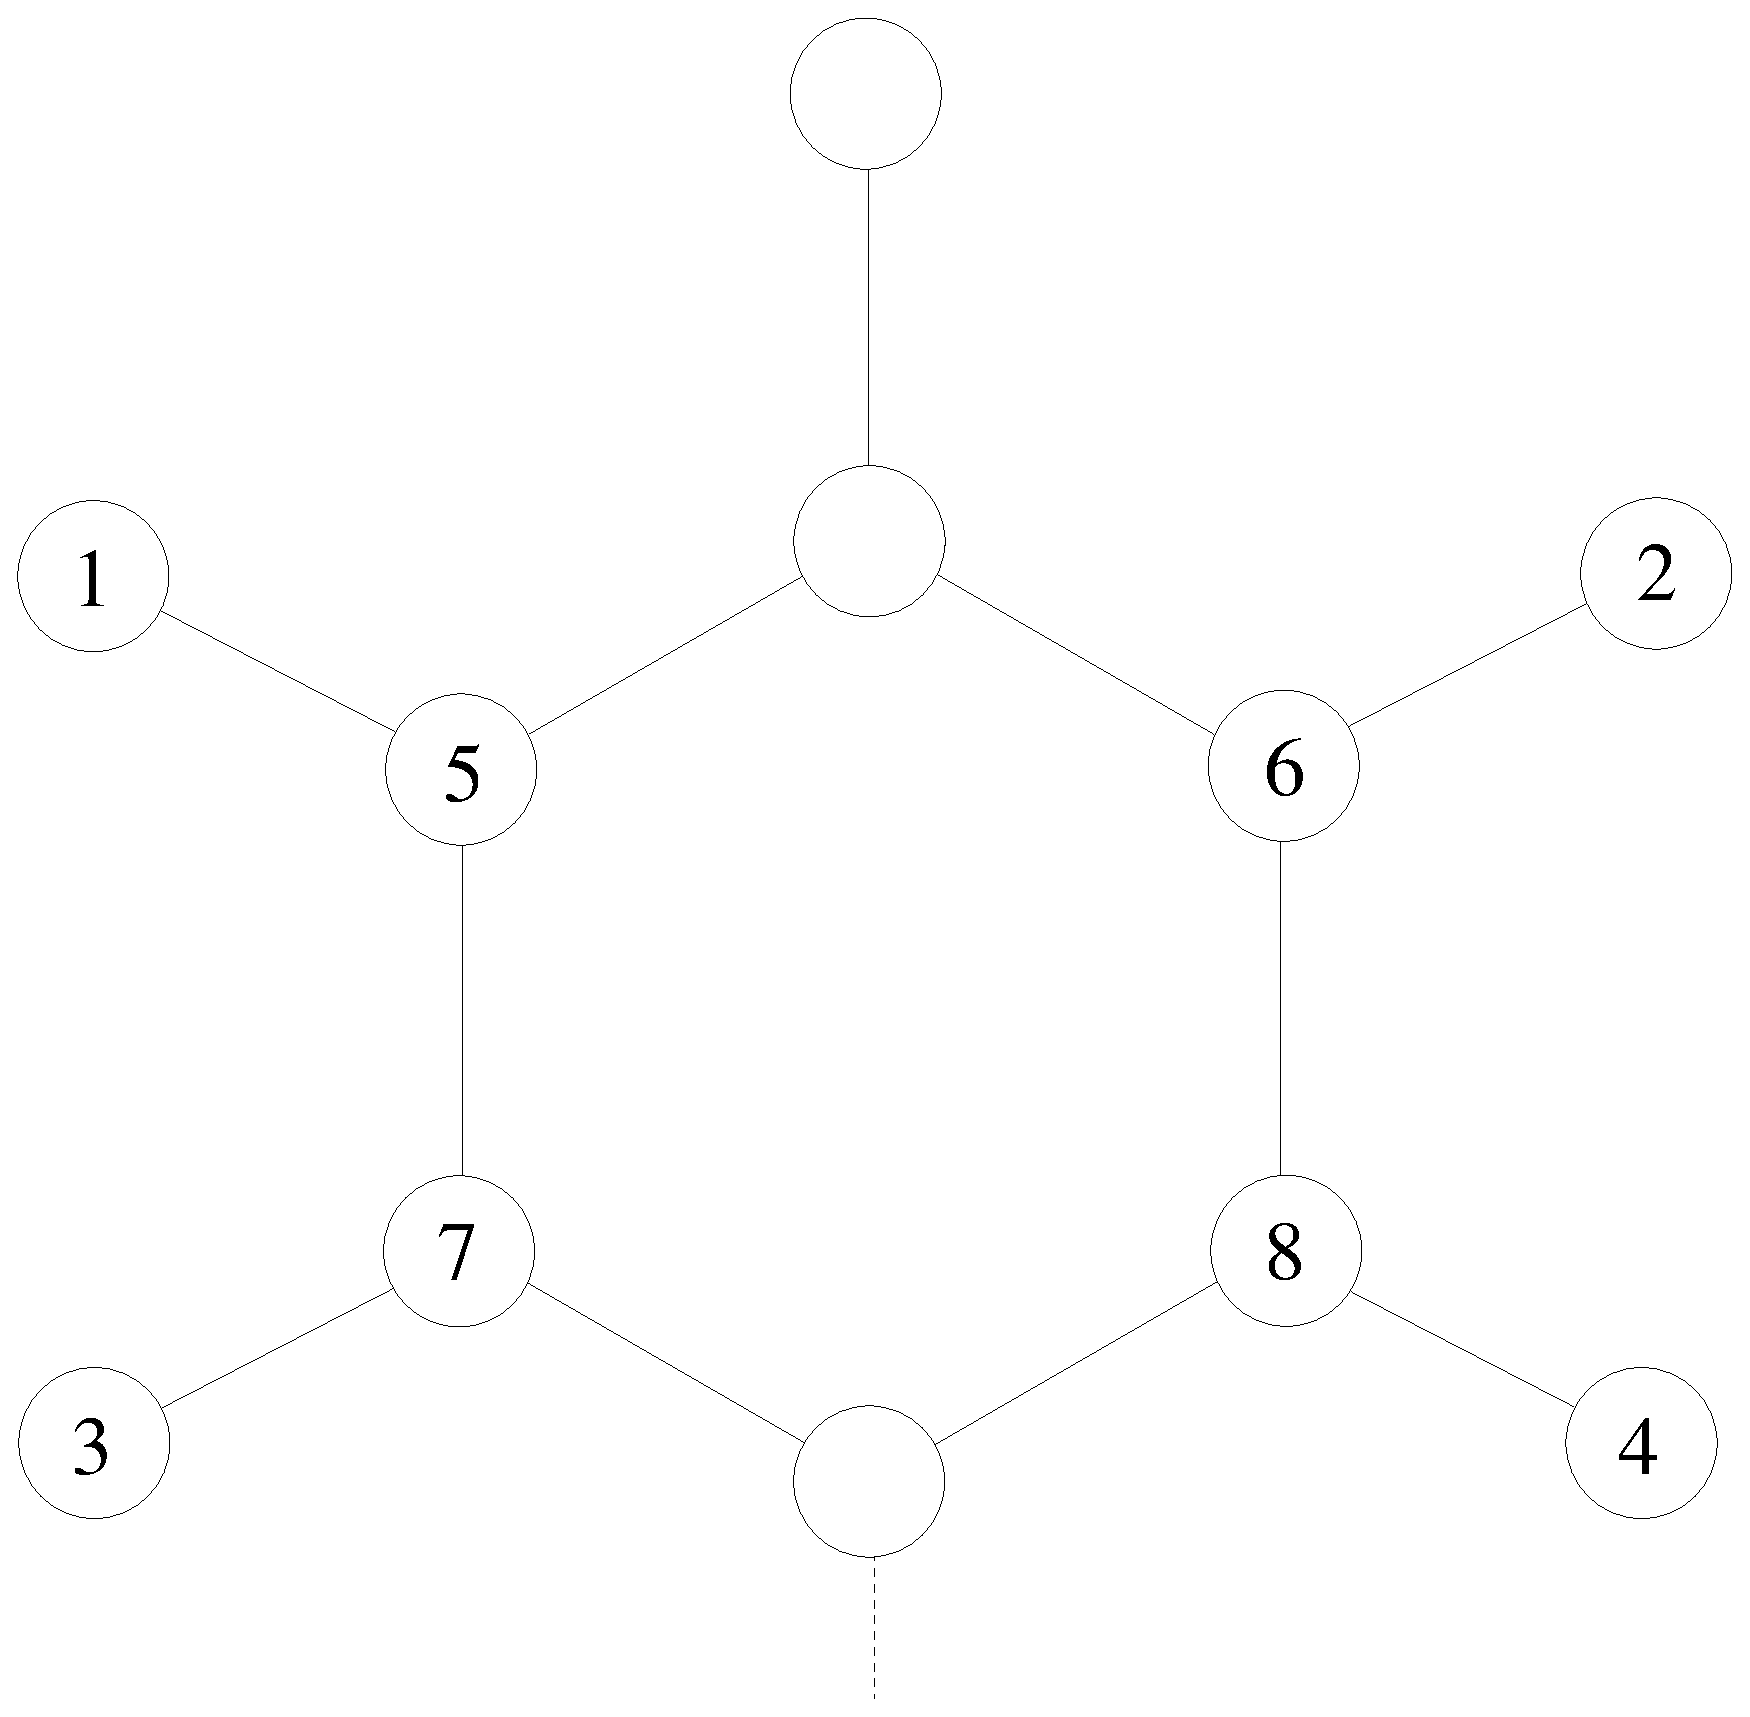
\includegraphics[width=0.5\textwidth]{PHE.eps}}
\end{figure}

For the phenylalanine example illustrated above we must allow three other pairs of
atoms to exchange if we swap 7 and 8. Hence a suitable {\tt perm.allow} entry is
{\obeylines
1
2 3
7 8 5 6 1 2 3 4
}
Here $n=2$ and $s=3$: if we exchange 7 and 8 then we must also exchange 5 and 6,
1 and 2, and 3 and 4. There are two atoms in each of the three secondary sets, 
since we have specified 7 and 8 as the two primary atoms.

Here is an example {\tt perm.allow} file for a water trimer using
the flexible {\keyw{QTIP4PF}} potential, where the energy is invariant to permutations
of water molecules and to exchanges of hydrogens in the same molecule. However,
hydrogens cannot exchange between different oxygens:
{\obeylines
4
3 2
1 4 7 2 3 5 6 8 9
2 0 
2 3
2 0 
5 6
2 0 
8 9
}
The first group of three oxygens has two atoms that must move with each oxygen,
i.e.~atoms 2 and 3 for oxygen 1, etc. Hydrogen permutations for each oxygen are
allowed by the three following groups. This scheme allows atoms to appear in more 
than one group. There must be a group containing each complete set of permutations
in order for permutation-inversion isomers to be recognised. The format
is compatible with an older scheme, where only pair swaps were allowed for
associated atoms, but now allows for more general permutations.

Scripts to generate allowed permutations automatically for CHARMM and AMBER are available from
the group web site. It is essential to use symmetrised versions of the corresponding
force fields! 

\ksec{PERTDIHE}{ chpmax chnmin chnmax iseed\/}: CHARMM 
and UNRES dihedral angle perturbation specification.
Performs random, {\tt GMIN}-style twists before starting optimisation.

\ksec{POINTS}{\/}: this is usually the last keyword and introduces the
coordinate information, which is read one atom per line. Each line must consist
of the atomic symbol of the atom followed by its three Cartesian coordinates.
Leading spaces before the atomic symbol should be avoided. For calculations
involving CHARMM, UNRES, AMBER and CPMD the coordinates are obtained from auxiliary files, 
and \keyw{POINTS} will be the last OPTIM directive in the {\tt odata} file, or
is not used (CHARMM and UNRES).

\ksec{PREROTATE}{\/}: For the GS and ES double-ended transition state
  search methods, if using {\keyw{FIXATMS}} to zero some coordinates of the
  forces to avoid overall translation and rotation, this keyword will rotate
  the start and end points so that those coordinates are zero in both.
The default is true.

\ksec{PRESSURE}{\/}: if present 
tells the program to perform a constant zero pressure optimisation
for bulk SC, ME, MP, MS and P6. Normally a constant volume optimisation takes place. 

\ksec{PRINT}{ n\/}: sets the print level. The default value is zero. Use
of this option is not recommended, since more specific print control is possible.

\ksec{PRINTCOEFFICIENTS}{\/}: prints ground state coefficients for the MSEVB potential.

\ksec{PULL}{ a1 a2 f\/}: apply a static force to the potential, equivalent to adding
the term $V_{\rm pull}=-f(z_{a1}-z_{a2})$. Here $z_{a1}$ and $z_{a2}$ are the $z$
coordinates for atoms $a1$ and $a2$, and $f$ specifies the force.
This potential is designed to simulate a pulling experiment with static force where
a molecule is pulled along the $z$ axis from atoms $a1$ and $a2$.

\ksec{PUSHCUT}{ x\/}: sets the threshold for the RMS force below which the
system may apply a {\keyw{PUSHOFF}} to escape from a stationary point of the wrong Hessian
index. Default value is 0.00001. Using a negative value prevents pushoffs from
occurring.

\ksec{PUSHOFF}{ x\/}: sets the magnitude of a step away from a stationary
point of the wrong Hessian index (see \S\ref{sec:scaling} for default action). Default value is 0.01.
Formally used as the step size in hybrid eigenvector-following
transition state searches if the eigenvalue of the direction being followed is positive.
{\keyw{MAXMAX}} has now replaced {\keyw{PUSHOFF}} in this role.

\ksec{PV}{ press gtol grad steps\/}: specifies an approximate constant pressure optimisation with
pressure {\it press\/} and convergence criterion {\it gtol\/} for the gradients with
respect to the box lengths. If any box length gradient is larger in magnitude than
{\it grad\/} then up to a maximum of {\it steps\/} optimisation steps for the box lengths
are performed.
If the three box lengths are equal to start with and the keyword {\keyw{CUBIC} \/} is included,
then a cubic box is maintained. 
Will not work with atom types MP, ME and MS.
Default values, {\it press\/}=0, {\it gtol\/}=0.001, {\it grad\/}$=10^{60}$, {\it steps\/}=100.

\ksec{PVTS}{ press gtol grad nboxts\/}: as for {\keyw{PV}} but searches for a transition
state with respect to box length {\it nboxts\/}, where {\it nboxts\/}=1, 2 and 3 specify the
$x$, $y$ and $z$ box lengths, respectively. {\it nboxts\/} defaults to 1.

\subsection{Q-R}
\ksec{QTIP}{4PF\/}: flexible water potential from  Habershon {\it et al.}~[{\it J.~Chem.~Phys.\/}, 
{\bf 131}, 024501 (2009)] coded by Dr Javier Hern\'andez-Rojas.
The units of length and energy are \AA\ and kcal/mol. The atoms must be entered in the
order O, H, H, O, H, H, etc.

\ksec{QSPCFW}{\/}: flexible water potential from  Paesani {\it et al.}~[{\it J.~Chem.~Phys.\/},
{\bf 125}, 184507 (2006)] coded by Dr Javier Hern\'andez-Rojas.
The units of length and energy are \AA\ and kcal/mol. The atoms must be entered in the
order O, H, H, O, H, H, etc.

\ksec{RADIUS}{ x\/}: specifies that atoms should not be allowed to move beyond a 
distance {\it x\/} from the origin.

\ksec{RANSEED}{ n\/}: specifies the initial seed for random number generation, as used in 
hard sphere moves with {\keyw{FIXD}}.

\ksec{RATIOS}{\/}: specifies that the pathway parameters needed to calculate catastrophe
ratios should be printed in a \keyw{PATH} run.

\ksec{RBSYM}{\/}: specifies that internal symmetry operations exist that permute
identical sites for rigid body building blocks. 
The operations are read in as the corresponding $3\times3$ matrices from a file
{\tt rbsymops}, which must exist in the working directory.
The first line of the file is an integer that specifies the number of operations; 
the matrix elements are then read in one at a time in free format.
This keyword can be combined with {\keyw{PERMDIST}\/} so that structures are aligned and
a distance metric considered based on permutations of identical rigid
bodies and any internal symmetry operation of each rigid body that is a symmetry
of the potential energy function.
We plan to extend this capability to assemblies containing more than one 
type of decorated rigid body.

\ksec{READPATH}{\/}: if specified with {\keyw{CALCRATES}} then rate constants will be
calculated for the transition states found in {\tt path.info} and no stationary point
searches will be performed.

\ksec{READSP}{\/}: instructs {\tt OPTIM} to read minima and 
transition state data in the {\tt PATHSAMPLE} format.
This has not been implemented yet!

\ksec{READHESS}{\/}: Hessian will be read from file {\tt derivs} at first step.

\ksec{READVEC}{\/}: if present the Hessian eigenvector
corresponding to the smallest eigenvalue 
will be read from file {\tt vector.dump}. The latter file can be generated using the
{\keyw{DUMPVECTOR}} keyword in a previous run.

\ksec{REDOPATH}{\/}: instructs {\tt OPTIM} to read transition state coordinates
successively from the file {\tt redopoints} during a \keyw{NEWCONNECT} run.
Can be used to generate movie files from stationary point sequences calculated
by {\tt PATHSAMPLE}. The correct start and finish coordinates for the minima
must be present in the {\tt odata} and {\tt finish} files.

\ksec{REDOPATHXYZ}{\/}: as for {\keyw{REDOPATH}} above, except that existing
{\tt path.n.xyz\/} files are read instead of actually calculating pathways for the
transition states.

\ksec{REDUCEDBONDLENGTH}{ blfactor CB\/}: rescales the bond lengths by a factor
of {\it blfactor} in the side chains of proteins, if modelled by one of the CHARMM
potentials. {\it blfactor} has to be specified, and its default value is one.
{\it CB} is an optional argument. When set, the bond length between the C$_{\alpha}$
and C$_{\beta}$ atoms is rescaled by {\it blfactor} as well, otherwise not.

\ksec{REOPT}{\/}: specifies that the eigenvector to be followed should be reoptimised
      in a BFGSTS search after the EF step and before the tangent space minimisation.
This is probably not a good idea. Default is false.

\ksec{REOPTIMISEENDPOINTS}{\/}: specifies that endpoint minima should be reoptimised
if their RMS force lies above the convergence threshold. Useful in connection 
runs where failure is guaranteed if one or more of the endpoints is not identified
as a minimum. A large RMS force at the beginning of a connection run driven
by {\tt PATHSAMPLE} should be investigated because it suggests a problem, e.g.~with
\keyw{CHARMM} permutational isomerisations.
Default is false.

\ksec{REPELTS}{\/}: specifies that the transition state search direction should
be orthogonalised to the coordinates in file {\tt points.repel}.

\ksec{RESIZE}{ x\/}: scales all the coordinates by {\it x}
before the first step is taken. 

\ksec{RING}{ a1 a2...}: When using natural internal coordinates, specifies
  a ring that's not part of a PRO, PHE, TYR, TRP, or HIS residue. {\it a1,
  a2}, etc. are the atom numbers for the ring in consecutive order. Only rings
  of size 5 or 6 are permitted.

\ksec{RKMIN}{ gmax eps\/}: calculates a steepest-descent path using gradient only
      information with convergence criterion {\it gmax\/} for the RMS force and initial
      precision {\it eps\/}. A fifth order Runga-Kutta algorithm is used.

\ksec{ROT}{\/}: if present a rotational kinetic energy term is
added to the Hamiltonian. Either constant angular momentum ({\keyw{ROT} JZ x\/}) or
constant angular velocity ({\keyw{ROT} OMEGA x\/}) may be used to specify $J_z$
or $\omega_z$.

% \subsection {\keyw{SAVE}CANDIDATES\/}: % unknown

\subsection{S}
\ksec{SCALE}{ n\/}: sets the scaling algorithm for eigenvector-following
steps, as described in \S\ref{sec:scaling}. The default is {\it n\/}=10.

\ksec{SCORE}{\_QUEUE\/}: specifies an Score parallel environment. 
Currently not used on group clusters.

\ksec{SEARCH}{ n\/}: specifies the search type for eigenvector-following and
steepest-descent calculations based on second derivatives and Hessian diagonalisation, default is type 0.
The most common options are 0, a minimisation, and 2, a transition state search. See
\S\ref{sec:second} for full details.

\ksec{SHIFT}{ x\/}: specifies the shift applied to eigenvectors corresponding
to normal modes that conserve the energy. The default is $10^6$. The shift {\it must\/} be
large enough to move the eigenvalues in question to the top of the spectrum.

\ksec{SQVV}{ NIterSQVVGuessMax SQVVGuessRMSTol\/}:
specifies that the first {\it NIterSQVVGuessMax\/} DNEB refinements should be
done using the SQVV algorithm, rather than LBFGS.\cite{TrygubenkoW04}
The DNEB optimisation will switch to LBFGS minimisation after {\it NIterSQVVGuessMax\/}
steps or if the RMS force falls below {\it SQVVGuessRMSTol\/}.
The default values for {\it NIterSQVVGuessMax\/} and {\it SQVVGuessRMSTol\/}
are 300 and 2.0, respectively.

\ksec{STEPMIN}{ n\/}: sets the minimum number of optimisation steps before convergence
will be tested. The default is zero.

\ksec{STEPS}{ n\/}: sets the maximum number of optimisation steps per call
to {\tt OPTIM}. The default is {\it n\/}=1. Setting {\it n\/} to zero at the start of a run
means that only a point group analysis is performed.

\ksec{STOCK}{ $\mu$ $\lambda$}: sets the dipole moment strength and attraction prefactor
in the Stockmayer potential,
\begin{displaymath}
V_{ij} = 4\left(r_{ij}^{-12}-\lambda r_{ij}^{-6}\right) + \frac{\mu^2}{r_{ij}^3}
\left[\hat{\pmb\mu}_i\cdot\hat{\pmb\mu}_j-\frac{3}{r_{ij}^2}
(\hat{\pmb\mu}_i\cdot{\bf r}_{ij})(\hat{\pmb\mu}_j\cdot{\bf r}_{ij})\right].
\end{displaymath}
See also {\keyw{STOCK}SPIN}.

\ksec{STOCKSPIN}{ x n}: Activates checking for alignment of dipoles with the $z$ axis in
the Stockmayer potential.  Such alignment makes the polar angle $\phi$ for the dipole
redundant, leading to extra zero Hessian eigenvalues and associated problems.  If alignment
is detected at any step in an optimisation then the orientation of the cluster is randomised
and a warning is printed.
$x$ is the amount by which $|\cos\theta|$ may differ from 1 for the dipole to be counted as
aligned with the $z$ axis.  $n$ is the maximum number of attempts to remove aligned dipoles
by random rotation.  Values of $10^{-4}$ and 10, respectively, are a sensible starting point.

\ksec{STOPDIST}{ x\/}: in a \keyw{CONNECT} run, stop as soon as the distance between
the initial ({\it x}$>0$) or final ({\it x}$<0$) minimum and the furthest connected minimum
exceeds $|x|$.

\ksec{STOPFIRST}{\/}: in a \keyw{CONNECT} run, stop as soon as the initial minimum has a transition state
connection.

\ksec{SUMMARY}{ n\/}: prints a summary of the steps and derivatives
every {\it n\/} steps. The default is $n=20$.

\ksec{SYMCUT}{ x\/}: specifies the RMS force below which the point
group symmetry subroutine will be called. The default is {\it x\/}=0.001.




\subsection{T-Z}
\ksec{TAG}{ num massfac\/}:
allows atoms to be tagged. Atom number {\it num\/} has its mass increased
by a factor {\it massfac\/} for point group symmetry assignment only.
To tag more than one atom use additional {\keyw{TAG}} lines in {\tt odata}.

\ksec{TD}{\/}: add a tetrahedral field of strength {\it x} to the potential.

\ksec{TOLD}{ x\/}: sets the initial distance tolerance for points
to be considered the same after rotations and reflections in point
group determination. The default is 0.0001.

\ksec{TIMELIMIT}{ x\/}: {\tt OPTIM} will stop if the accumulated cpu
time exceeds {\it x} seconds. The default value is infinity.

\ksec{TOLD}{ x\/}: initial distance tolerance in symmetry subroutine.
The default is 0.0001.

\ksec{TOLE}{ x\/}: sets the initial tolerance for eigenvalues
of the inertia tensor to be considered equivalent in point
group determination. The default is 0.0001.

\ksec{TOMEGA}{\/}: includes omega angles in the {\keyw{TWISTDIHE}} list.

\ksec{TOSI}{ $A_{++}\ A_{--}\ A_{+-}\ \rho$\/}: specifies a Born-Mayer potential
with the parameters indicated (see \S\ref{sec:potentials}).

\ksec{TOSIC}{6 c6pp c6mm c6pm\/}: specifies additional C6 dispersion coefficients
for the {\keyw{TOSI}\/} potential. {\it c6pp, c6mm\/}, and  {\it c6pm\/} should be the values of the C6
parameters between positive ions, negative ions and positive and negative ions in atomic units
(see \S\ref{sec:potentials}).

\ksec{TOSIPOL}{ alphap alpham damp\/}: specifies cation and anion polarisabilities in atomic units
and a damping parameter for the {\keyw{TOSI}\/} potential (see \S\ref{sec:potentials}).

\ksec{TRAD}{ x\/}: sets the trust radius (see \S\ref{sec:scaling}). The default value is 2.0.

\ksec{TRAP}{ k n\/}: general trapped ion potential coded by Ersin Yurtsever. 
The form of the potential is 
\begin{displaymath}
V=\frac{k}{2}\sum_i r_i^n + \sum_{i<j} \frac{1}{r_{ij}},
\end{displaymath}
where $r_i$ is the distance of ion $i$ from the origin and
$r_{ij}$ is the distance between ions $i$ and $j$.

\ksec{TSIDECHAIN}{\/}: includes sidechain angles in the {\keyw{TWISTDIHE}} list.

\ksec{TWISTDIHE}{ nmode xpert\/}: twist phi/psi dihedral angle {\it nmode\/} by 
{\it xpert\/} degrees before starting optimisation.

\ksec{TWISTTYPE}{ n\/}: integer {\it n\/} specifies the type of dihedral angle twisting
used to  guess transition states in {\bf guessts} for CHARMM and UNRES.
The recommended value is {\it n}=5. See also {\keyw{NORANDOM}}.

\ksec{TWOENDS}{ fstart finc ntwo rmstwo ntwoiter twoeval\/}: obsolete: specifies a double-ended transition
state search. {\it fstart\/} is the initial force constant pulling the coordinates towards the final
geometry which is read from a file named {\tt final}. {\it finc\/} is the increment for the force 
constant after each cycle. {\it ntwo\/} is the maximum number of minimisation steps taken after each
increment of the force constant, and {\it rmstwo\/} is the convergence condition on the RMS force
for these minimisations. {\it ntwoiter\/} is the total number of force constant increments allowed
and {\it twoeval\/} is the value of the smallest Hessian eigenvalue below which the program will
shift to a transition state search.

\ksec{UACHIRAL}{\/}: MUST be included when using ff03ua, the AMBER united atom forcefield. It ensures the correct impropers are used to define sidechain 
chirality when HB hydrogen is missing.

\ksec{UNRES}{\/}: specifies the UNRES potential, which requires an UNOPTIM executable.
An auxiliary file {\tt coords} is required. {\keyw{UNRES}} must be the last OPTIM directive in the
{\tt odata} file. The remaining content of {\tt odata} consists of UNRES keywords and
setup information.

\ksec{UPDATES}{ mupdate1 mupdate2 mupdate3 mupdate4\/}: 
specifies the number of updates in the LBFGS routine before
      resetting. 
{\it mupdate1\/} is used for energy minimisation, 
{\it mupdate2\/} is currently ignored by {\bf mind},
{\it mupdate3\/} is used in Rayleigh-Ritz eigenvalue calculations, and 
{\it mupdate4\/} is used in NEB and DNEB optimisation. 
{\it mupdate5\/} is used in string method optimisation. 
The default value is 4 for all five parameters.

\ksec{USEDIAG}{ n\/}: allows different approximations to be used for the 
eigenvalue in a Rayleigh-Ritz {\keyw{BFGSTS}} calculation. $n=1$ is the default behaviour
with lower truncation error,
while $n=2$ uses a formula that minimises the rounding error, which may
work better for numerically large values of the energy.

\ksec{USEEV}{ n \/}: specifies the number of non-zero (lowest) eigenvalues and
eigenvectors to be calculated by LAPACK routine DSYEVR in {\bf efol.f},
{\bf bfgsts.f} or {\bf hybridmin.f}.
If this value is not specified than full diagonalisation is performed in 
{\bf efol.f} using LAPACK routine DSYEV, while the default is a single
eigenvalue/eigenvector for {\bf bfgsts.f} and {\bf hybridmin.f}.

\ksec{VALUES}{ n\/}: prints the Hessian eigenvalues every {\it n\/} steps.
The default is {\it n\/}=20.

\ksec{VARIABLES}{\/}: optimises a general function (which must be specified in
{\bf potential}. The initial values of the variables are read one per line after the \keyw{POINTS}
keyword in {\tt odata}.

\ksec{VECTORS}{ n\/}: prints the Hessian eigenvectors every {\it n\/}
steps. Eigenvector printing is turned off by default.

\ksec{WARRANTY}{\/}: print warranty information.

\ksec{WELCH}{ $A_{++}\ A_{--}\ A_{+-}\ \rho\ Q_+\ Q_-\ \alpha_+\ \alpha_-$\/}: specifies a Welch binary
salt potential with the parameters indicated (see \S\ref{sec:potentials}).

\ksec{ZEROS}{ n\/}: sets the number of zero Hessian eigenvalues to be
assumed---useful for general optimisation problems specified by {\keyw{VARIABLES}}. 
%\end{itemize}
% </kwd>

\section{Specification of Potentials}
\label{sec:potentials}
There follows a list of some of the 
potentials that the program understands. These are introduced according to the atom
type by which they are identified.

\subsection{AR}Lennard-Jones potential with $\sigma$ appropriate for Ar,
i.e.~$3.4\,$\AA. Hence, input is expected in Angstrom and energies are calculated
for $\epsilon=1$. Subroutines used: {\bf ljdiff}.

\subsection{AU, AG and NI}These types specify Sutton-Chen potentials of the appropriate
form.\cite{suttonc90}\ 
Three additional real parameters must be specified using the {\keyw{PARAMS}} keyword
in the {\tt odata} file,
namely Sutton and Chen's $\epsilon$, $c$ and $a$, in this order.
The nearest neighbour distance in the prevailing unit system is $a/\sqrt{2}$. Hence,
using $a=\sqrt{2}$ corresponds to a unit system where the bulk nearest-neighbour distance is 1.
Subroutines used: {\bf scdiff}.

\subsection{AX}Lennard-Jones potential plus a variable quantity of the Axilrod-Teller
triple-dipole term\cite{wales90c,doyew92}\ with units $\sigma=\epsilon=1$. 
The pre-multiplication factor for
the three-body term, $Z^*$, is specified by the {\keyw{PARAMS}} keyword.
If a multiplier of $0.0$ is specified the Axilrod-Teller derivatives
and energy are not calculated, thus providing a route to the pure Lennard-Jones potential
in reduced units. Subroutines used: {\bf ardiff}, {\bf apairs}, {\bf axdiff}, {\bf axpairs}.

\subsection{AZ}Aziz argon potential from {\it J.~Chem.~Phys.\/}, {\bf 99}, 4518, 1993.
Input coordinates are assumed to be in units of $\sigma$ and the energy is given in
units of $\epsilon$.

\subsection{BC}Binary Lennard-Jones system, as for atom type LS, but without periodic
boundary conditions. Subroutine used: {\bf ljpshiftbinc}.

\subsection{BE}This specifies a trapped ion potential.\cite{walesl93}\
Subroutines used: {\bf etrap}, {\bf dtrap}.

\subsection{C1}A ten-bead model produced by cutting down the usual P46 potential specified
by atom type PL. Subroutine used: {\bf c10}.

\subsection{C6}This type specifies Girifalco's C$_{60}$ intermolecular potential.\cite{girifalco92}\
The energy is returned in units of the pair well depth; distances are in units of $3.4690\,$\AA.
Subroutines used: {\bf c60diff}.

\subsection{CADPAC}If keyword {\keyw{CADPAC}} is set in {\tt odata} then
OPTIM will try to read the derivatives from file {\tt derivs} in the
standard CADPAC\cite{CADPAC}\ punch format. 
It will also try to read the energy for the geometry
corresponding to these derivatives from a file called {\tt cadenergy}, which is optional.

\subsection{CC}This uses the two- plus three-body potential of Balm \etal\ for carbon.\cite{balmakm91} 
Subroutines used: {\bf jmecc}, {\bf jm2cc}, {\bf jm3cc}.

\subsection{CD}Specifies a potential for rigid-body pentagonal pyramids. In this case the
rigid body coordinates are three centre-of-mass parameters and three components of a 
vector that specifies a rotation axis and magnitude. The orientational coordinates are stored
after all the centre-of-mass coordinates. Subroutine used: {\bf capsid}.

% \subsection{CL}This is used to specify a Born-Meyer potential for $\rm (KCl)_n$ clusters
% using the same parameters as Rose and Berry.\cite1\ 
% \endnote{J.~P.~Rose and R.~S.~Berry}{\jcp}{96}{517}{1992}
% The atoms must be in the order K, Cl,
% K etc. Atomic units are assumed. Subroutines used: {\bf kdiff}, {\bf kpairs}.

\subsection{CK}Specifies a two-dimensional trapped-ion cluster. Subroutines used:
{\bf ectrap} and {\bf dctrap}.

\subsection{DZ}Dzugutov potential:\cite{Dzugutov92,Dzugutov93b}
\begin{eqnarray}
V(r)&=&A(r^{-m}-B) \exp\left( {c\over r-a}\right) \Theta(a-r) + 
    B \exp\left({d\over r-b}\right) \Theta(b-r). \nonumber
\end{eqnarray}
Seven parameters must by specified by a {\keyw{PARAMS}} line in the {\tt odata} file,
i.e.~$m$, $A$, $c$, $a$, $B$, $d$, and $b$.

\subsection{FH}Will read derivatives from file {\tt fhderivs} generated by the Fenske-Hall approximate
SCF package.\cite{hallf72}

\subsection{GAUSSIAN}If keyword {\keyw{GAUSSIAN}} is set in {\tt odata} then
OPTIM will try to read the derivatives from file {\tt derivs} in the
standard GAUSSIAN punch format.
It will also try to read the energy for the geometry
corresponding to these derivatives from a file called {\tt cadenergy}, which is optional.

\subsection{GL}This type specifies a G\={o}-type model\cite{uedatg78} for the
46-bead three-colour model polypeptide specified by atom type Pl below. 
All the attractive $1/R^6$ terms are turned off except for those between
native contacts in the global minimum, which are unchanged.
Subroutines used: {\bf g46merdiff}.

\subsection{GO}Paul Whitford's G\={o} BLN-type potential.

\subsection{IN}This is used to specify a shielded Born-Meyer potential binary ionic clusters with
anions and cations having the same magnitude charge.
The atoms must be in the order cation, anion, cation, anion, etc. The energy is:
$$ E = \sum_{i<j} \left[ {q_iq_j\over r_{ij}} e^{-\gamma r_{ij}} + A_{ij}e^{-r_{ij}/\rho_{ij}} \right]. $$
The parameters that can
be specified with {\keyw{PARAMS}} are $\gamma$, the magnitude of the ionic charges, a single
value of $\rho$, assumed to be the same for all interactions, and $A_{++}$, $A_{--}$ and
$A_{+-}$, in order. Default values for KCl are set for all parameters except $\gamma$.
Atomic units are assumed. Subroutines used: {\bf ions}.

\subsection{JC}This uses Murrell's two- plus three-body 
potential.\cite{murrellm90,murrellr90,alderzijmr91,eggenjlm92,fengjm93} 
A file {\tt JMparams} must
exist in the current directory containing the parameters $c_0,\ c_1,\ldots,\ c_{10},\ r_e,\ 
D,\ a_2$ and $a_3$. Subroutines used: {\bf jmec}, {\bf jm2c}, {\bf jm3c}.

\subsection{JM}This uses Murrell's two- plus three-body 
potential\cite{murrellm90,murrellr90,alderzijmr91,eggenjlm92,fengjm93} with periodic boundary
conditions (minimum image convention.\cite{allent87} 
A {\tt JMparams} file must exist as for type JC. (In previous versions the 
first three lines of {\tt JMparams} were assumed to contain
the square roots of 2, 3 and 6). Four additional real parameters must be given after the
search type and maximum step size specification, these being the $x$, $y$ and $z$ dimensions
of the periodic cell and the cutoff, respectively. I do not think the code has been tested
for any non-cubic unit cells. The cutoff should not be greater than half the box length.\cite{allent87}
Subroutines used: {\bf jmep}, {\bf jm2p}, {\bf jm3p}.

\subsection{LM}Specifies a Mason-Schamp potential\cite{Mason58} for a rare gas--alkali metal ion cluster
such as Ar$_{N}$Li$^+$. The three parameters $\epsilon$, $R_m$ and $\gamma$
must be set using the {\keyw{PARAMS}} keyword in {\tt odata}.

\subsection{LP}This type specifies the Lennard-Jones potential with 
periodic boundary conditions (minimum image convention.\cite{allent87}
The box lengths in the $x$, $y$ and $z$ 
directions and the cutoff (as a fraction of the smallest box length)
must be specified using the {\keyw{PARAMS}} keyword in the {\tt odata} file.
Setting a negative value for the cutoff fraction means that all minimum
images are included.
Subroutines used: {\bf ljpdiff}.
If the {\keyw{BINARY}} keyword is specified then a binary Lennard-Jones
potential is used\cite{sastryds98} along with subroutine {\bf ljpbin} or {\bf ljpshift}.

\subsection{LS}This type specifies shifted, truncated Lennard-Jones potential with 
periodic boundary conditions as for LP above. The {\keyw{BINARY}} keyword must also be 
specified.

\subsection{LC}This type specifies shifted, truncated Lennard-Jones potential with 
periodic boundary conditions, as for LS above, except that the neighbour list is not
updated when FIXIMAGE is set. The {\keyw{BINARY}} keyword must also be 
specified. See also {\keyw{FIXAFTER}}.

\subsection{LM}Lennard-Jones potential with a mean-field long range correction.

\subsection{M}This specifies a Morse potential with $D=r_e=1$. 
The remaining range parameter,\cite{braierbw90} $\rho_0$, must be specified using the {\keyw{PARAMS}} keyword
in the {\tt odata} file.
Subroutines used: {\bf mpairs}, {\bf mdiff}.

\subsection{ME}Specifies the generic Mie potential with periodic boundary conditions (minimum
image convention). Six extra parameters must be specified in the {\tt odata} file using the
{\keyw{PARAMS}} keyword;
in order these are the exponents {\it n\/} (repulsive) and $m$ (attractive), the three box
lengths and the cutoff. If keyword {\keyw{PRESSURE}} is set in {\tt odata}
then a constant pressure type optimisation is performed
using golden section minimisation, as described for SC. Note that
{\it n\/} and {\it m\/} should both be entered as reals. Subroutines used: {\bf emie}, {\bf mied}
and {\bf miel}. 

\subsection{MP}This type specifies the Morse potential with 
periodic boundary conditions (minimum image convention\cite{allent87}). 
The range parameter, $\rho_0$, the box lengths in the $x$, $y$ and $z$ 
directions and the cutoff (as a fraction of the smallest box length)
must be specified using the {\keyw{PARAMS}} keyword in the {\tt odata} file.
If the keyword {\keyw{PRESSURE}} is set in the {\tt odata} file
then a constant pressure optimisation is performed
with the energy being minimised by eigenvector-following with respect to the 
box lengths at every step. 
The cutoff is automatically changed in proportion to the change in box size.
Otherwise the optimisations are performed at constant volume, with no 
relaxation of the unit cell. 
Subroutines used: {\bf mpdiff}, {\bf mlatmin}.

\subsection{MS}This type specifies the Morse potential with 2-dimensional
periodic boundary conditions.
The free surfaces are perpendicular to the $z$ direction at the top and bottom
of the cell.
The range parameter, $\rho_0$, the box lengths in the $x$ and $y$ 
directions and the cutoff (as a fraction of the smallest box length)
must be specified using the {\keyw{PARAMS}} keyword in the {\tt odata} file.
If the keyword {\keyw{PRESSURE}} is set in the {\tt odata} file
then a constant pressure optimisation is performed
with the energy being minimised by eigenvector-following with respect to the 
box lengths at every step. 
The cutoff is automatically changed in proportion to the change in box size.
Otherwise the optimisations are performed at constant volume, with no 
relaxation of the unit cell. 
Subroutines used: {\bf msdiff}, {\bf mslatmin}.

\subsection{P6}This type specifies Girifalco's C$_{60}$ intermolecular potential\cite{girifalco92}
with periodic boundary conditions (minimum image convention\cite{allent87}). If keyword
{\keyw{PRESSURE}} is specified in {\tt odata}
then a constant pressure type optimisation is performed,
as described for SC, above. However, in this case the lattice constant optimisation is
achieved by eigenvector-following. As for SC, the cutoff is changed in proportion to
the box size. Four extra parameters must be specified in the {\tt odata} file using the
{\keyw{PARAMS}} keyword,
as for SC. Subroutines used: {\bf latmin}, {\bf c60p}.

\subsection{PL}This type specifies a 46-bead three-colour model polypeptide. 
See also the corresponding G\={o} model potential.
Subroutines used: {\bf p46merdiff}.

\subsection{PR}This type specifies the Pacheco-Ramelho C$_{60}$ intermolecular potential\cite{pachecor97}
The value of the Axilrod-Teller parameter should be specified as the first argument to the
PARAMS keyword.

\subsection{SC}This type specifies the Sutton-Chen potential\cite{suttonc90} with periodic boundary
conditions (minimum image convention\cite{allent87}). 
If no file named {\tt SCparams} exists in the current 
directory the 12\mydash6 potential for gold is used. Otherwise the Sutton-Chen
parameters $n,\ m,\ \epsilon,\ c$ and $a$ are read from this file in order. If the
keyword {\keyw{PRESSURE}} is set in the {\tt odata} file
then a constant pressure optimisation is performed
with the energy being minimised by golden section with respect to the cubic box size before taking another
step. The cutoff is automatically changed in proportion to the change in box size.
Otherwise the optimisations are performed at constant volume, with no relaxation of the
unit cell. The bulk fcc nearest neighbour distance in the prevailing unit system is $a/\sqrt{2}$,
as above.
Subroutines used: {\bf escp}, {\bf dscp}.

\subsection{SI}This uses Murrell's two- plus three-body potential for Si\cite{lijm92}.
Subroutines used: {\bf jme}, {\bf jm2}, {\bf jm3}.

\subsection{SM} Specifies the Stillinger-Weber two- plus three-body potential for Si\cite{stillingerw85}
with the three-body part increased by 50\%.
Subroutines used: {\bf SWtwo}, {\bf SWthree}, {\bf SWlatmin}.

\subsection{SW} Specifies the Stillinger-Weber two- plus three-body potential for Si\cite{stillingerw85}.
Subroutines used: {\bf SWtwo}, {\bf SWthree}, {\bf SWlatmin}.

\subsection{Tosi}This keyword specifies a Born-Mayer potential of the form
$$ E = \sum_{i<j}\left[ {q_i q_j\over r_{ij}} + A_{ij}\exp(-r_{ij}/\rho) \right]. $$
The sum runs over all ions. Tosi-Fumi\cite{tosif64} parameters in atomic units should be
entered after the Tosi keyword in the order $A_{++}$, $A_{--}$, $A_{+-}$, $\rho$.
The ions are then specified using atom types PL and MI for plus and minus, respectively,
and can be in any order. There need not be equal numbers of positive and negative ions.
C6 dispersion coefficients can be optionally added with the keyword {\keyw{TOSI}C6 c6pp c6mm c6pm\/},
where {\it c6pp, c6mm\/}, and  {\it c6pm\/} should be the values of the C6 parameters between positive ions,
negative ions and positive and negative ions in atomic units. First order induction energy
can be added with the keyword {\keyw{TOSIPOL} alphap alpham damp\/} where {\keyw{ALPHA}P\/} and
{\keyw{ALPHA}M \/} are the cation and anion polarisabilities in atomic units and {\it DAMP\/}
is the damping parameter, without which cold fusion is likely. Note that the Welch potential
has been fitted to include ion polarisabilities and is described below.

% \subsection{TB}Tersoff-Brenner potential for carbon\cite1---numerical second derivatives only.
% \endnote{D.~W.~Brenner}{J.~Phys.~Rev.~B}{42}{9458}{1990}
% Subroutines used: {\bf tbe}, {\bf tbdiff}.

\subsection{TH} Specifies the Thomson problem. Two times the number of ions
must be divisible by three.

\subsection{TT} Specifies a tight-binding potential. 
Subroutines used: {\bf tighte}, {\bf secsi}.

\subsection{Welch}This keyword specifies a Welch potential\cite{welchld76,phillipscb91} of the form
\begin{eqnarray*}
E &= \sum_{i<j}\Bigg[ {\D q_i q_j\over\D  r_{ij}} + A_{ij}\exp(-r_{ij}^{\rm eff}/\rho) 
              -{\D q_i({\bf \mu}_j\cdot{\bf r}_{ij})\over\D  r_{ij}^3} 
              -{\D q_j({\bf \mu}_i\cdot{\bf r}_{ji})\over\D  r_{ij}^3} \\
             &-3{\D   ({\bf \mu}_i\cdot{\bf r}_{ij})
                   ({\bf \mu}_j\cdot{\bf r}_{ij})\over\D  r_{ij}^5} 
              +{\D  {\bf \mu}_i\cdot{\bf \mu}_j\over\D  r_{ij}^3}\Bigg] 
              +\sum_i {\D \mu_i^2\over\D 2\alpha_i}, \\
\end{eqnarray*}
where 
$$ {\bf r}_{ij}^{\rm eff}={\bf r}_{ij}+{{\bf\mu}_i\over Q_i}-{{\bf \mu}_j\over Q_j}, 
    \qquad r_{ij}^{\rm eff}=\left|{\bf r}_{ij}^{\rm eff}\right|. $$
Welch parameters in atomic units should be
entered after the Welch keyword in the order $A_{++}$, $A_{--}$, $A_{+-}$, $\rho$, $Q_+$,
$Q_-$, $\alpha_+$, $\alpha_-$.
The ions are then specified using atom types PL and MI for plus and minus, respectively,
and can be in any order. There need not be equal numbers of positive and negative ions.

\subsection{W1, W2, W3, W4}Specifies that each {\tt odata} entry gives the centre of mass coordinates
of a rigid water molecule to be described by a TIPS potential\cite{jorgensen81} of type 1, 2, 3 or 4.
The Euler angles then follow all the centre of mass coordinates, again three per line.
Subroutines used: {\bf h2o}.

\subsection{Z1, Z2}These are the two forms of the Zetterling potential:\cite{DoyeWZD03}
\begin{equation}
V(r)=a {e^{\alpha r}\over r^3} \cos(2k_F r)+b\left({\sigma\over r}\right)^{n}+V_0.
\end{equation}
Subroutines used: {\bf Z1} and {\bf Z2} etc.
If three parameters are specified by the {\keyw{PARAMS}} keyword they are interpreted 
as box lengths for a periodic system.

% \subsection{A1, A2, A3, A4}Used for a benzene-Ar$_n$ cluster with four slightly different
% potentials. In each case the benzene molecule has a fixed geometry which is not read in.
% Potentials for A1 and A3 include the induction energy, while A2 and A4 do not. Potentials
% A1 and A2 use one set of Lennard-Jones parameters while A3 and A4 use a different set\cite1.
% \endnote{D.~J.~Wales}{\molphys}{74}{1}{1991}
% Subroutines used: {\bf bzgeom}, {\bf bzarlj}, {\bf ljdiff}, {\bf bzarin}, {\bf indiff}.

\subsection{Rotating Clusters}If keyword {\keyw{ROT}} is set in 
{\tt odata} then additional terms will be added to the
energy and the derivatives corresponding to the kinetic energy for rigid body rotation
about the space fixed $z$ axis. Either the angular momentum or the angular velocity
may be fixed using {\keyw{ROT} J2Z\/} or {\keyw{ROT} OMEGA2\/} followed by the value.

\section{Second-Derivative Based Searches}
\label{sec:second}
At present there are eight possible single-ended search types 
that employ Hessian calculation (or update) and full diagonalisation. They are specified by
the \keyw{SEARCH} keyword with a parameter 
represented by the internal integer variable INR, with allowed values ranging from 0 to 7. 
The two most common
types are 0, for minimisation, and 2, for transition state searching. The steps have
the same form in both cases,\cite{wales94a} except that we go downhill in every direction when
minimising, and uphill in one direction when looking for a transition state. For these
search types convergence to stationary points with the wrong Hessian index (i.e.~not
0 or 1 negative Hessian eigenvalues, respectively) is detected and countermeasures are
taken as specified below. 

The eigenvector to be followed `uphill'
in an eigenvector-following transition state search is specified by an integer following the keyword 
{\keyw{MODE}} in {\tt odata}.  We count up from the eigenvector corresponding to 
the smallest eigenvalue, the one corresponding to the second smallest eigenvalue 
etc.~using values 1, 2 and so on. The value specified by {\keyw{MODE}} is only
effective on the first step: for subsequent steps the critical eigenvector is 
chosen by a maximum overlap criterion using the dot product with the eigenvector 
that was followed at the previous step.  Using {\keyw{MODE}} 0 means that the 
eigenvector corresponding to the smallest Hessian eigenvalue is chosen at every step. 

Quite often, especially if we are taking large steps in a region far from convergence,
the largest modulus dot product may fall well below unity and give rise to ambiguity.
At present the program takes the following action if the maximum overlap is less than
0.7. The chosen eigenvector is simply set to the same one that was followed in the last
step, where the eigenvectors are numbered in terms of the corresponding eigenvalues arranged in
ascending order. Zero eigenvalues are excluded from the counting. The same action is
taken if the maximum overlap is with an eigenvector lying more than 8 places above
the one followed at the previous step, when arranged according to ascending eigenvalue.

The behaviour for other search types is as follows. \keyw{SEARCH} 1
specifies a pseudo-Newton-Raphson search where the formula for the steps is the same
as the eigenvector-following step for search types 0 and 2, but we search uphill or
downhill depending only upon the sign of the eigenvalue corresponding to the direction
in question.\cite{wales94a}
Of course, this step tends to the conventional Newton-Raphson step
near a stationary point. For \keyw{SEARCH} 1 convergence to stationary points of any Hessian 
index is allowed.

Search types 3 and 4 are the same as 0 and 2 except that a pseudo-third derivative
correction is applied to the step\cite{wales94a}. These search types are now {\bf redundant}
because dynamic scaling using a trust radius and separate maximum step sizes for each
direction seems to work much better (see \S\ref{sec:scaling}).

Search type 5 is the same as type 0 except that the system is rotated into principal
axes first.

Search types 6 and 7 are for steepest-descent energy minimisations using the Page-McIver
method\cite{pagem88} with analytic first and second derivatives at each step. 
Search type 7 can converge to a saddle point, search type 6 can only converge to a true minimum.

Search type 8 is a steepest-ascent transition state search using a modification of
the Page-McIver steepest-descent algorithm.

Search types 0, 6 and 7 can be used as minimisers for pathway calculations.
In this case it is possible to use a subset of eigenvalues and eigenvectors
by supplying {\keyw{USEEV} n \/} in {\tt odata}.
The number of second derivative-based minimisation steps can be controlled
with {\keyw{PATH}SDSTEPS n\/}, after which {\tt OPTIM} will switch to LBFGS.

\section{Gradient-Only and Hybrid Searches}
\label{sec:gradient}
It is generally much more efficient to carry out energy minimisation, including
pathway calculations, using the LBFGS gradient-only routine specified by
{\keyw{BFGSMIN}}. Steepest-descent
paths or minimisations can also be calculated by Runge-Kutta or Bulirsch-Stoer integration
using the {\keyw{RKMIN}} and {\keyw{BSMIN}} keywords, respectively.

A hybrid BFGS/eigenvector-following
transition state search\cite{munrow99,kumedamw01} can be specified by {\keyw{BFGSTS}}. In this approach
an eigenvector-following step is taken along the eigenvector corresponding to
the smallest eigenvalue, which is determined by iteration if second derivatives are
available, or a variational method if not ({\keyw{NOHESS}}). 
LAPACK routine { DSYEVR} is used to find only the lowest required Hessian eigenvalues
and eigenvectors if {\keyw{NOIT}} is specified.
LBFGS minimisation is performed in the tangent space following uphill eigenvector-following
steps, but it is not necessary for
this optimisation to converge accurately except in the vicinity of the transition state.
There are therefore two maximum values for the number of LBFGS steps
allowed in the tangent space optimisation: one is used when the eigenvalue does
not appear to have converged, the other when it has. See the {\keyw{BFGSTS}} keyword.
If the Hessian is relatively cheap to calculate, but the system size is large, then
Hessian diagonalisation should be avoided using {\keyw{BFGSTS}}.
If the smallest eigenvalue is positive then the uphill step size is set to the value
specified by the keyword {\keyw{MAXMAX}}.

The Hessian index can be checked after an LBFGS or hybrid search by calculating 
eigenvalues iteratively until the smallest positive eigenvalue is found. Checking is
turned on by the keyword {\keyw{CHECKINDEX}}. This keyword now works with {\keyw{NOHESS}}.

Pathways can be calculated by stepping off a transition state using an eigenvector-following
step along the eigenvector corresponding to the smallest Hessian eigenvalue calculated
by iteration, followed by LBFGS minimisation. The keyword {\keyw{BFGSSTEP}}
must be specified to do this. If the {\keyw{PUSHOFF}}
parameter is set then it is used in the usual way. The sign of the {\keyw{MODE}} parameter,
if set, specifies whether the initial step is parallel or antiparallel to the
eigenvector located. However, the \keyw{PATH} keyword now provides a much simpler way
to calculate complete paths.

\subsection{Eigenvalue Shifting}In versions of OPTIM prior to 1999
projection was used to remove displacements corresponding to 
overall translations and rotations where necessary.\cite{bakerh91,wales93d}
From April 1999 projection was replaced by eigenvalue shifting where the
eigenvalues corresponding to eigenvectors which conserve the energy
are moved to the top of the spectrum. This procedure seems to be simpler
and more efficient, especially in terms of memory. A new keyword {\keyw{SHIFT}}
was introduced, which enables the upward shift to be adjusted if required.
For systems involving periodic boundary conditions no shifting should really be
needed, but there is little overhead for doing so and the program is simpler.
For trapped ion clusters
rotation-only shifting is used. If keyword {\keyw{ROT}} is specified then shifting is performed
only for the eigenvalues corresponding to
rotations around the space-fixed $z$-axis. Otherwise shifting is applied to the
eigenvalues corresponding to both $z$ translation and rotation.

The program can cope with linear molecules (including diatomics) so long as all the atoms
are not in the $z=0$ plane. However, linear molecules and {\keyw{ROT}} will not work.

\section{Running OPTIM}
\label{sec:running}
Any number of optimisation steps can be run with a
single call to OPTIM, as specified by the keyword {\keyw{STEPS}}.
The default convergence criteria for eigenvector-following and steepest-descent runs are
that the maximum unscaled step size for
any coordinate (or eigenvector, depending upon the scaling criterion) is less
than $10^{-5}$ and the RMS force is also less than $10^{-5}$.
The number of negative Hessian eigenvalues must also agree with the search type requested.
These convergence criteria can be overruled by the 
{\keyw{CONVERGE}} keyword, as described in \S\ref{sec:keywords}.

\section{Step Scaling Criteria}
\label{sec:scaling}
Once an eigenvector-following step of whatever
type has been calculated it will generally need to be scaled down. Five methods
are available for doing this, as set by the keyword {\keyw{SCALE}}. 

For {\keyw{SCALE}} 0 the `step length' is taken to be the total step length in the multidimensional
space of Cartesian coordinates. For {\keyw{SCALE}} 1 we scale according to the largest displacement
in Cartesian coordinates. For {\keyw{SCALE}} 2 we scale according to the largest displacement
in the Hessian eigenvector basis. For {\keyw{SCALE}} 3 we scale according to the total step size
called for by the steepest-descent routine. The default for all other \keyw{SEARCH} types is now
{\keyw{SCALE}} 10 for which a different trust ratio is calculated for each eigendirection and used 
to adjust the maximum allowed step for each eigenvector. This
is described in more detail below.\cite{walesw96}

{\keyw{SCALE}} 10 employs a trust radius whose default value is 4.0. This value can be changed
using the keyword {\keyw{TRAD}}.
{\it Appropriate values for the maximum initial step size and the trust radius
for different systems may need to be found by experimentation\/}. After the first step the
program compares the predicted value of the Hessian eigenvalue for a given eigendirection,
as calculated by finite difference of the present and previous component of the gradient in
this direction, with the actual eigenvalue. The trust ratio for a particular eigendirection
is the modulus of this predicted value minus the actual value, divided by the actual value. 
If the trust ratio is less than the trust radius then the maximum step allowed in this
direction is increased by a factor of $1.1$ (up to a maximum of 0.5); if it is more
than the trust radius the maximum allowed step in this direction is divided by $1.1$ (down
to a minimum allowed value of $0.005$). The maximum allowed step for each direction is
initialised at the value read from the {\tt odata} file. 

The trust ratio is not used in a transition state search for the uphill direction if the 
corresponding eigenvalue is positive; the step size is instead set to the value
of the {\keyw{MAXMAX}} parameter.

This trust ratio approach assumes that all the eigenvectors are in correspondence for the present and
previous geometries when they are arranged according to the eigenvalues in ascending or
descending order. When large steps are being taken some eigendirections are likely to cross
over, and it might be better to use an overlap criterion for all the present and previous
eigenvectors. However, this has not proved to be necessary to date.

Scaling of the above sort does not apply in :BFGS minimisations, although the
trust radius approach described above for {\keyw{SCALE}} 10 is used for the eigenvector-following
step in hybrid transition state searches.

For \keyw{SEARCH} 0, 2, 3 and 4 OPTIM detects convergence to stationary points with the
wrong Hessian index and steps away from them. The test is triggered when the RMS force
falls below the value specified by {\keyw{PUSHCUT}} (default $10^{-5}$)
in the prevailing units. The test is only applied at the first step and every fourth step. 
If a transition state search converges to (or starts from) a minimum
a step is taken in the direction specified by {\keyw{MODE}} of magnitude {\keyw{PUSHOFF}}.
If {\keyw{PUSHOFF}} has not been set then the displacement is one tenth of the
current maximum step size allowed for the eigenmode in question.
If a transition state
search converges to (or starts from) a higher index saddle then the action depends upon the
value of {\keyw{MODE}}. For {\keyw{MODE}} 0 displacements are taken for all the eigenmodes
with negative eigenvalues except for the one with the most negative eigenvalue. The magnitude
of the displacement is determined in the same way as above.
For {\keyw{MODE}} $n\not=0$ a displacement is applied only along the specified value of {\keyw{MODE}}.
For search types 0 and 3 similar action is taken. If the search converges to (or starts from)
a stationary point that is not a minimum then if {\keyw{MODE}} 0 displacements are applied
for all the eigenmodes with negative eigenvalues. If {\keyw{MODE}} $n\not=0$ then a displacement
is only applied in the direction specified by {\keyw{MODE}}.

\section{Point Group Determination}
\label{sec:symmetry}
The eigenvalues
of the moment of inertia tensor are first inspected to see if there should be a principal
rotation axis of order 3 or more. Degeneracy is assumed if the difference between two principal
moments of inertia, divided by the trace of the inertia tensor, is less than some tolerance,
which is initially set to $0.005$. This tolerance can be changed with the keyword {\keyw{TOLE}}.
Symmetry elements are then sought depending upon this first
result, and are diagnosed when rotation or reflection operations produce the same geometry
correct to $0.01$ in each Cartesian coordinate. This tolerance can be changed with the
keyword {\keyw{TOLD}}. If symmetry elements expected for the
calculated principal moments of inertia are not found then the first tolerance is divided by
ten and the whole procedure repeated with a warning message about `accidental degeneracy'. 
If the first tolerance falls below $10^{-7}$ the routine gives up.

Point group determination should work for small molecules belonging to all point groups with 
principal axes of order less than 6. Higher order rotation axes can be sought using the
keyword {\keyw{AXIS}}. Problems due to the tolerances occur for larger molecules,
particularly those with high symmetry. 

\section{Calculating Pathways}
\label{sec:pathways}
Having found a transition state it is possible to
find the corresponding minima (and pathway) by displacing the transition state along
the transition vector in both senses and starting minimisations for each point. To make
a complete path the data from one of these searches must be reversed and the results
for the other side of the path appended to it. Shell scripts to do this automatically
for all the transition states in a given directory, and to perform miscellaneous analysis
of the pathways, exist for various potentials. The \keyw{PATH} keyword should now be
used to calculate complete pathways given a transition state geometry in {\tt odata}.
Characteristics of the path, such as barrier heights, distances and the cooperativity index,
are then produced automatically, along with a file containing the energy as a function
of integrated path length (in {\tt EofS}) and an xyz file containing the specified number
of frames on each side of the path (in {\tt path.xyz}).

Pathways are calculated by starting a minimisation of some sort after stepping off the
transition state specified in {\tt odata}.
Using {\keyw{MODE}} values of 1 and $-1$ will give the two sides of the path.
With \keyw{SEARCH} 0 (or 3) or LBFGS minimisation 
the resulting pathway will only be an approximation to a true
gradient line. For search type 6 (or 7) and {\keyw{RKMIN}} or {\keyw{BSMIN}} 
the results should be close to the true steepest-descent
path. Note that gradient lines are properties of the potential energy surface alone, and
do not depend upon masses. Mass weighting, or calculating pathways in the fictitious
space with a kinetic metric,\cite{banerjeea92} has now been implemented, but not in the BFGS
minimisation or hybrid EF/BFGS routines.

\section{Double-Ended Searches}
\label{sec:double}
OPTIM.2.3 introduced two keywords to provide double-ended pathway searches.
The first is \keyw{NEB}, 
an implementation of the revised nudged elastic band approach.\cite{HenkelmanJ00,HenkelmanUJ00}
The second is \keyw{CONNECT}, which can also find pathways connecting two minima using a different
strategy. In both cases the coordinates of the starting minimum are specified in the {\tt odata} file,
and the coordinates of the final minimum are specified in the file {\tt finish}.
\keyw{CONNECT} builds up a complete min-sad-min-$\cdots$-min sequence by systematically 
searching for transition
states and calculating pathways. The \keyw{PATH} keyword is not needed, but can be used to change the
number of points files saved in the {\tt path.$n$.xyz} files, which are saved for each transition state, $n$.
The energy profiles are saved in files EofS.$n$.

If \keyw{CONNECT} needs to connect permutational isomers of the same minimum in the
course of a run then the initial guess for the transition state geometry is generated
using the \keyw{NEB} routine with just two images, to avoid cold fusion problems.

\keyw{CONNECT} generally needs to be augmented by other keywords to specify how the transition
state geometries should be guessed (\keyw{NEB},
\keyw{NEWNEB} or {\keyw{FIXD}}), how the transition
state searches should be performed ({\keyw{SEARCH} 2\/} or {\keyw{BFGSTS}}, with or
without {\keyw{NOHESS}}, {\keyw{NOIT}} etc.), and how that pathways should be
calculated ({\keyw{SEARCH} 0,\/} 6 or 7, {\keyw{BFGSMIN}}, {\keyw{RKMIN}} or {\keyw{BSMIN}}).
Most of these combinations should work together.
A summary file will be produced if {\keyw{DUMPPATH}} is specified. An xyz file
for the overall path will be printed to {\tt path.xyz} and the energy as a
function of path length is printed to {\tt EofS}. The corresponding xyz and energy
files for the individual steps in the path are numbered path.$n$.xyz and EofS.$n$ for
transition state $n$.

When \keyw{NEB} is used in a \keyw{CONNECT} run its function is merely to produce a
starting guess for the transition state geometry, from which a transition state search
of some kind is then initiated. It seems that the higher energy parts of a path converge 
faster than the lower regions in \keyw{NEB} calculations, and so it is possible to generate
a transition state guess using only a few images and sloppy convergence in the \keyw{NEB}
part of the calculation.

In the latest OPTIM the \keyw{NEB} and \keyw{CONNECT} keywords are augmented by new algorithms,
which are selected using \keyw{NEWNEB} and \keyw{NEWCONNECT}. \keyw{NEWNEB} can work on its
own and with both \keyw{CONNECT} and \keyw{NEWCONNECT}. However, \keyw{NEWCONNECT}
cannot be used with the old \keyw{NEB}.
The new algorithms are based on the doubly-nudged elastic band approach and a 
more sophisticated connection algorithm.\cite{TrygubenkoW04}

The latest double-ended search methods to be implemented correspond to the
\keyw{GROWSTRING} and \keyw{EVOLVESTRING} keywords, which provide implementations of the
growing string and evolving string methods.\cite{ERV02,PetersHBC04}

\section{Output}
\label{sec:output}
The amount of information printed can be controlled
through the keywords {\keyw{GRADIENTS},\ VECTORS,\ EFSTEPS,\ VALUES,\ SUMMARY,\/}
and {\keyw{DEBUG}} as described in \S\ref{sec:keywords}.
Some useful aliases to interrogate output files are:

\medskip
\begin{tabular}{l}
alias energy $'$grep $''$Energy for last$''$ output!$\star$$'$ \\
alias unscaled $'$grep unscaled output!$\star$$'$ \\
alias RMS $'$grep RMS output!$\star$$'$ \\
alias pgroup $'$grep group output!$\star$$'$ \\
alias negative $'$grep negative output!$\star$$'$ \\
\end{tabular}

\section{Auxiliary Programs}
\label{sec:auxiliary}
As mentioned above there exist numerous shell scripts
and fortran programs designed to do specific tasks such as analysis of pathways,
finding transition states for a given minimum or for a directory full of minima and
calculating pathways for a transition state or a directory full of transition states.
Some of these were superceded from OPTIM.2.3 onwards by new keywords like \keyw{PATH}
and \keyw{CONNECT}, which allow OPTIM to perform multiple stationary point searches 
in one call. The Filthy\_Phyllis program can be used to build up a connected database of
transition states and local minima, and generally lives up to her name.
PATHSAMPLE is a program that employs OPTIM to perform discrete path sampling
calcualtions.\cite{Wales02,Wales03}

\section{Example {\tt odata} Files}
\label{sec:examples}
The first example is for an eigenvector-following 
transition state search with maximum step size and  trust radius different from the default
values. The eigenvector corresponding to the second-lowest non-zero eigenvalue is followed
uphill at the first step, with subsequent uphill directions being determined by the overlap
condition. The convergence criteria are an unscaled maximum step size of 0.005 and an RMS
gradient tolerance of 0.000001. 

\medskip
\begin{tabular}{ll}
 SEARCH & 2  \\
 MODE & 2 \\
 MAXSTEP & 0.1  \\
 TRAD & 2.0  \\
 STEPS & 100  \\
 CONVERGE & 0.005 0.000001  \\
 POINTS  \\
 etc.  \\
\end{tabular}
\medskip

\noindent The next dataset is the same as above except that we perform an eigenvector-following
minimisation and set an initial displacement from the assumed transition state of
0.05 units.

\medskip
\begin{tabular}{ll}
 SEARCH & 0 \\
 PUSHOFF & 0.05 \\
 MAXSTEP & 0.1 \\
 TRAD & 2.0 \\
 STEPS & 100 \\
 CONVERGE & 0.005 0.000001 \\
 POINTS \\
 etc. \\
\end{tabular}
\medskip

\noindent Next is an LBFGS energy minimisation with a maximum of 100 steps and
convergence conditions of 0.00001 for the RMS gradient.
There follows a check of the Hessian index using iteration to calculate 
eigenvalues to an accuracy of 0.01 with 200 and 50 iterations maximum for the smallest
and largest eigenvalues, respectively. A Hessian will be calculated in order to 
perform the check. {\keyw{NOIT}} could be used, in which case the lowest ten Hessian
eigenvalues will be calculated. If {\keyw{NOHESS}} is specfified then the smallest
non-zero Hessian eigenvalue will be calculated variationally.

\medskip
\begin{tabular}{ll}
 STEPS & 100 \\
 BFGSMIN & 0.00001 \\
 CHECKINDEX & 200 0.01 50 \\
 POINTS \\
 etc. \\
\end{tabular}
\medskip

\noindent Next is a transition state search using the hybrid EF/BFGS method. The maximum EF
step and trust radius are 0.1 and 2.0, respectively,
and the maximum step in the LBFGS tangent space minimisation is 0.2. The maximum number of combined
EF/BFGS steps is 100. The maximum number of iterations allowed is
200 for the smallest and 50 for the largest eigenvalue. A maximum of 20 BFGS steps 
is permitted in
the orthogonal subspace after each eigenvector-following step until the eigenvalue
appears to have converged, when the maximum jumps to 100 steps.
The convergence criterion
for the Hessian eigenvalues is that the percentage change between steps is
less than 0.01. The convergence criterion for each BFGS
subspace minimisation 0.0001 for the RMS gradient.
Setting {\keyw{PUSHOFF}} to 0.1 enables us to start from a converged minimum with
a large step.
Convergence is achieved when the maximum unscaled eigenvector-following step
falls below 0.01, the total RMS force falls below 0.0001, and the previous subspace
minimisation has converged. The smallest eigenvalue and the corresponding eigenvector
are saved in file {\tt vector.dump}. The Hessian index is checked using iteration to
calculate the eigenvalues with the same parameters as the {\keyw{BFGSTS}} keyword.
Note: if the RMS tolerance specified by {\keyw{BFGSCONV}} is larger than that specfied by
{\keyw{CONVERGE} \/} the algorithm cannot converge.

\medskip
\begin{tabular}{ll}
 MAXSTEP & 0.1 \\
 MAXMAX  & 0.1 \\
 MAXBFGS & 0.2 \\
 PUSHOFF & 0.1 \\
 TRAD & 2.0 \\
 STEPS & 100 \\
 BFGSTS & 200 20 100 0.01 50 \\
 BFGSCONV & 0.0001 \\
 CONVERGE & 0.01 0.0001 \\
 DUMPVECTOR \\
 CHECKINDEX \\
 POINTS \\
 etc. \\
\end{tabular}
\medskip

\noindent The following {\tt odata} file is the same as above, except that no Hessian is
available. A maximum of 30 steps is permitted in the BFGS Rayleigh-Ritz
minimisation, which is designed to produce the lowest eigenvalue, and the
convergence condition on this eigenvalue is that the RMS force in the variational BFGS
minimisation falls below 0.1.
Otherwise the parameters have the same meanings as above.
The maximum step size in the Rayleigh-Ritz minimisation is set to 0.2 by the
{\keyw{MAXBFGS}} keyword.

\medskip
\begin{tabular}{ll}
 MAXSTEP & 0.1 \\
 MAXMAX  & 0.1 \\
 MAXBFGS & 0.2 0.2 0.2 \\
 PUSHOFF & 0.1 \\
 TRAD & 2.0 \\
 STEPS & 100 \\
 NOHESS \\
 BFGSTS & 30 20 100 0.1 \\
 BFGSCONV & 0.0001 \\
 CONVERGE & 0.01 0.0001 \\
 DUMPVECTOR \\
 CHECKINDEX \\
 POINTS \\
 etc. \\
\end{tabular}
\medskip

\noindent Next we calculate the part of the reaction pathway
resulting from a displacement of 0.05 antiparallel to the transition
vector saved in file {\tt vector.dump}. 
The calculation reverts to a pure LBFGS minimisation after the first step.

\medskip
\begin{tabular}{ll}
 MAXSTEP & 0.1 \\
 MAXBFGS & 0.1 \\
 TRAD & 2.0 \\
 STEPS & 100 \\
 PUSHOFF & 0.05 \\
 MODE & $-1$ \\
 READVEC \\
 BFGSSTEP \\
 BFGSCONV & 0.0001 \\
 CONVERGE & 0.01 0.001 \\
 POINTS \\
 etc. \\
\end{tabular}

\noindent The next example shows how to calculate a complete pathway from the transition state geometry
specified in {\tt odata} reading the eigenvector from file {\tt vector.dump}. 
{\keyw{NOIT}} or {\keyw{NOHESS}} could also be specified in conjunction with {\keyw{BFGSTS}}. 
Alternatively, {\it READVECTOR\/} would cause the required eigenvector to be read from 
file {\tt vector.dump}; in this case either {\keyw{BFGSSTEP}} or {\keyw{BFGSTS}} must
also be present in {\tt odata}.
The maximum LBFGS step is set to 0.05; this setting
helps to make the path smoother and generally gives a closer approximation to the true steepest-descent
path. The LBFGS convergence criterion is that the RMS force falls below 0.000001. {\keyw{BFGSMIN}}
could be replaced by {\keyw{RKMIN}} or {\keyw{BSMIN}} to obtain more accurate steepest-descent paths.

\medskip
\begin{tabular}{ll}
PATH & \\
MAXBFGS & 0.05 \\
STEPS & 500 \\
BFGSTS & 500 10 10 0.01 500 \\
PUSHOFF & 0.04 \\
BFGSMIN & 0.000001 \\
DUMPPATH \\
POINTS & \\
 etc. \\
\end{tabular}

\noindent Pathways can also be calculated using entirely second derivative based steepest-descent methods:

\medskip
\begin{tabular}{ll}
PATH &\\
CONVERGE& 0.01 0.000001\\
STEPS&  500\\
SEARCH& 5\\
PUSHOFF&  0.04 \\
DUMPPATH& \\
POINTS& \\
etc. & \\
\end{tabular}

\noindent Alternatively, the eigenvector for which a {\keyw{PUSHOFF}} is required can be calculated by a full
diagonalisation of the Hessian followed by a gradient only based minimisation:

\medskip
\begin{tabular}{ll}
PATH &\\
CONVERGE& 0.01 0.000001\\
STEPS&  500\\
SEARCH& 0\\
BFGSMIN & 0.00001 \\
PUSHOFF&  0.04 \\
DUMPPATH& \\
POINTS& \\
etc. & \\
\end{tabular}

\noindent A more complicated example for a \keyw{CONNECT} run using \keyw{NEB} to generate transition
state guesses and {\keyw{BFGSTS}} for transition state searches. {\keyw{NOIT}}  or 
{\keyw{NOHESS}} could also be used in conjunction with {\keyw{BFGSTS}}. The maximum number of 
transition state searches allowed is 20, and {\keyw{BFGSTS}} searches are started from 
guesses generated by \keyw{NEB} using a small number of images and a sloppy convergence
criterion. Pathways will be calculated by LBFGS energy minimisation with 2000 steps allowed, 
whereas only 300 steps are allowed in the transition state searches.

\medskip
\begin{tabular}{ll}
CONNECT &  20 \\
NEB     &  100 5 0.02 \\
PATH    &  3 \\
BFGSTS  &  100 3 20 0.01  \\
BFGSMIN & 0.000001 \\
PUSHOFF  & 0.05 \\
BFGSSTEPS & 2000 \\
STEPS     & 300 \\
POINTS & \\
etc. & \\
\end{tabular}

\noindent In the next example hard sphere moves are used for the initial transition state guesses, using a 
displacement vector based upon the initial and final geometries of the two minima in question 
at the given step, if they are initially less than 2.5 distance units
apart. Steepest-descent pathways are calculated by Runge-Kutta integration.

\medskip
\begin{tabular}{ll}
CONNECT & 30 \\
PATH   &  3 \\
FIXD & 0.70 2.5 \\
BFGSTS  & 100 3 20 0.01 \\
BFGSCONV & 0.000001 \\
RKMIN & 0.00001 0.1 \\
NOIT & \\
PUSHOFF & 0.05 \\
STEPS     & 2000 \\
POINTS & \\
etc. & \\
\end{tabular}

\noindent The pathways can also be calculated using the Page-McIver second-order steepest-descent approach:

\medskip
\begin{tabular}{ll}
CONNECT & \\
NEB     &  100 5 0.02 \\
PATH    &  3 \\
SEARCH & 6 \\
MAXSTEP & 0.05 \\
MAXMAX  & 0.1 \\
TRAD & 1.0 \\
BFGSTS  & 100 3 20 0.01  \\
BFGSCONV & 0.000001 \\
NOIT & \\
PUSHOFF & 0.05 \\
STEPS   &  2000 \\
POINTS & \\
etc. & \\
\end{tabular}

\noindent A collection of example {\tt odata} and the corresponding output files can be
found in the {\tt newtests} directory.


\chapter{PATHSAMPLE}
\renewcommand{\pname}{PATHSAMPLE}

\section{Introduction}
\label{sec:intro}

{\tt PATHSAMPLE.2.1} is the current version of the {\tt OPTIM} driver program to implement a
discrete path sampling (DPS) construction of stationary point 
databases and perform kinetic analysis.\cite{Wales02}\cite{Wales03,Wales04,TrygubenkoW06,Wales06}
This implementation provides a number of different methods for growing stationary 
point databases in order to produce samples that are kinetically relevant.
The main difference from {\tt PATHSAMPLE.2.0} is that the geometrical test for
distinguishing stationary points has been changed to use the minimum distance.
This usage is consistent with {\tt OPTIM} and the tolerance is set using the
keyword {\keyw{GEOMDIFFTOL}}. Subsequent enhancements of the code are not implemented
in {\tt PATHSAMPLE.2.0}.

{\tt PATHSAMPLE} relies upon {\tt OPTIM} \cite{optim} to perform geometry optimisation, 
especially double-ended searches for pathways between specified minima. 
In the simplest case, all the {\tt OPTIM} calls will be Dijkstra connect runs
\cite{CarrTW05} (this is the case if the {\keyw{CONNECT}IONS} parameter is less than or equal to one,
see \S \ref{sec:keywords}).
Please refer to the {\tt OPTIM} documentation for full details of this program \cite{optim}.

The DPS technique is designed to calculate rate constants
between two different regions (A and B) on the potential energy surface, 
where a region is defined by a set of local minima.\cite{Wales02,Wales03,Wales04,TrygubenkoW06,Wales06,
EvansW03b,EvansW04,CarrW05}
In {\tt PATHSAMPLE.2.0} and above, this objective is achieved by building up
a stationary point database using successive double-ended connection runs between
local minima, where connections are chosen according to the minimum distance 
between the minima and their predicted committor probabilities.
Note that that this approach is different from the original philosophy,
which focused upon the rates associated with individual discrete paths and created 
new paths by perturbing old ones.

% <changes>
\section{Recent Changes}
\label{sec:latest}

The {\keyw{NGT}} keyword has been added for a new graph transformation procedure. 
This routine can calculate $k^{\rm SS}$, $k^{\rm NSS}$ and $k^{\rm KMC}$ for both
$A\leftarrow B$ and $B\leftarrow A$, as well as committor probabilities, in one call.
This is now the recommended way to calculate rate constants.

The {\it DIJINIT\/} keyword has been replaced by two separate keywords,
namely {\keyw{DIJINITSTART}\/} and {\keyw{DIJINITCONT}\/}, to simplify the generation of
initial paths. 

{\keyw{DIJINITSTART}\/} is intended for automatic setup of the {\tt min.A}, {\tt min.B},
{\tt min.data}, {\tt ts.data}, {\tt points.ts} and {\tt points.min} files from initial
{\tt odata.start} and {\tt odata.finish} files. In contrast to the previous 
philosophy, {\keyw{DIJINITSTART}\/} will {\bf overwrite database files if they already exist}.
Hence it is possible to wipe an existing database with this keyword.

{\keyw{DIJINITCONT}\/} is intended for continuation of initial path searches that have not yet 
completed. It can also be used to start a run if the required database entries for two
end points have been created by hand. {\keyw{DIJINITCONT}\/} will check that the required
files are present in the current working directory, and stop if they are not.

The MFPT calculation for the fastest steady-state path (ignoring recrossings)
in a {\keyw{DIJKSTRA}} calculation
has been changed to the graph transformation approach.\cite{TrygubenkoW06}

The printing of rate constants at the end of a {\keyw{GT}\/} calculation has been changed
to make it clear which values are calculated assuming that detailed balance holds.
An extra summary line with the non-detailed balance rate constants is printed at the end.

After each cycle over the available CPU's {\tt PATHSAMPLE} will now check to see if the
file {\tt pathdata.change} exists in the current working directory. 
If it does, then {\tt pathdata.change} is copied to {\tt pathdata}
and all parameters are reread using {\bf keyword}.
This feature is designed to allow for change of parameters during a run without
the need to kill and requeue a job. 
Attempts to change variables that affect declarations of array bounds will 
cause the program to crash.

%</changes>
\section{Input files}
\label{sec:input}
The following files are required in the directory where {\tt PATHSAMPLE} is executed.
\smallskip
\begin{itemize}
\item {\tt pathdata}: contains parameters to control the stationary point
sampling and/or the kinetic analysis. See \S\ref{sec:keywords}.
\item {\tt odata.*} files: the {\tt odata} file is the control file for {\tt OPTIM}. 
One {\tt odata} file is
needed for each type of {\tt OPTIM} job performed by {\tt PATHSAMPLE}. See \S\ref{sec:odatafiles}.

\item {\tt commit.data}. This file is updated every time a committor probability 
calculation is performed. Initial committor probabilities are read from it if the
file is detected. Otherwise, the initial values are 
set to zero and one as appropriate.
If a {\tt PATHSAMPLE} run ends abnormally it is possible for the number of entries
in {\tt commit.data} to be less than the number of local minima in {\tt min.data}.
In this case the missing values are automatically
set to zero. This procedure does not work with some compilers
if they behave incorrectly on reaching the end of file.
In this case the missing zeros can simply be added using a text editor.

\end{itemize}

The following files may be required, depending upon the keywords set in {\tt pathdata}:
\smallskip
\begin{itemize}
\item {\tt min.A}, {\tt min.B} and {\tt min.data}: lists of A, B and intermediate minima, respectively. 
The first line of {\tt min.A} is the number of A minima (free format), $N_{\rm A}$; on the following lines
there must be $N_{\rm A}$ integers (free format), which specify all the local minima 
belonging to the A set. Hence, the A region can be changed simply by editing this file.
{\tt min.B} has the same format for the B minima.
The numbering of the local minima must be consistent with the order of their
coordinates in {\tt points.min} (see below).
However, unlike older versions of {\tt PATHSAMPLE}, the A and B minima can appear 
in any order, facilitating regrouping schemes.
The file {\tt min.data} has the format:

{\it energy\quad frequency\quad pgorder\quad itx\quad ity\quad itz}

for each minimum, where $energy$ is the potential energy (as calculated by {\tt OPTIM}), 
$frequency$ is the natural log of the
product of positive eigenvalues from the mass-weighted Hessian
(used to evaluate partition functions and rates constants), $pgorder$ is the order of the point group,
and $itx, ity, itz$ are the (sorted) eigenvalues of the inertia tensor.
The order of entries in {\tt min.data} must agree with the {\tt min.A},
{\tt min.B} and {\tt points.min} files.

\item The file {\tt ts.data} is analogous to the {\tt min.data} file, 
but contains data for the transition states. The format is: 

{\it energy\quad frequency\quad pgorder\quad min1\quad min2\quad itx\quad ity\quad itz} 

where the entries are the same as for the minima, with the addition of {\it min1} and
{\it min2}, which identify the minima that the transition state connects. 
This file must be consistent with {\tt points.ts} (see below).

\item {\tt points.min}: contains the Cartesian coordinates of all the minima that are specified in 
{\tt min.data} in the same order. It is 
an unformatted direct access file, written with the Fortran specifier 
{\tt RECL=8*3*NATOMS}. 

\item {\tt points.ts}: as for {\tt points.min}, but contains the transition state 
coordinates.

\item {\tt nodes.info}: must be present for runs on a distributed memory machine.
The first line must contain an integer equal to the number of nodes available,
and the names of these nodes must follow below. 
On the final line the userid must be provided.
An example script for the qsub command could look like:
\begin{table}[H]
\begin{center}
\begin{tabular}{l}
\#!/bin/csh \\
\#PBS -q h4 \\
cd \$PBS\_O\_WORKDIR \\
cat \$PBS\_NODEFILE $>$\& output \\
wc output $>$ nodes.info \\
cat \$PBS\_NODEFILE $>>$ nodes.info \\
echo \$USER $>>$ nodes.info \\
/home/bin/pathsample $>>$\& output \\
\end{tabular}
\end{center}
\end{table}

\item {\tt path.info.startup}: an {\tt OPTIM} {\tt path.info}
file from a connect run that connects an A minimum to a B minimum.
Note that an output file is not required, unlike older versions of {\tt PATHSAMPLE}.
This file is needed to
provide an initial path, and the file name startup is specified in the {\tt pathdata} file
by the {\keyw{STAR}TFROMPATH} keyword.
If the files {\tt min.A} and {\tt min.B} are absent, then {\keyw{STAR}TFROMPATH}
will create them, with a single minimum specified in each region, corresponding
to the entries specified on the {\keyw{STAR}TFROMPATH} line after the file extension
startup.
The rest of the minima read from the
{\tt path.info.startup} file will be placed in the intervening set.
Note that for {\tt path.info} files in the new {\tt OPTIM}
{\keyw{DUMP}ALLPATHS} format, the two end point minima will generally not
be the first and last entries.
Since {\tt min.data} contains only unique minima, whereas the {\tt path.info} file may have
duplicates, the positions of the starting and finishing minimum may not be obvious.
A quick way to check these values is to run {\tt PATHSAMPLE} first with {\keyw{CYCLES} 0},
find the positions of the two minima in {\tt min.data} and correct
the values in {\tt pathdata}, remove {\tt min.*}, {\tt points.*}
and {\tt *.data}, and start the real {\tt PATHSAMPLE} run.
If the {\tt path.info.startup} file is in the new {\keyw{DUMP}ALLPATHS} format
then {\tt pathdata} must contain the keyword {\keyw{STAR}TTRIPLES}.
For a setup where the A and B sets are predefined in {\tt min.A} and {\tt min.B}
a connecting pathway can be read using the keyword {\keyw{ADDPATH} add} in {\tt pathdata}.
A path will then be read from file {\tt add}; if this path is
in the new {\keyw{DUMP}ALLPATHS} format then the keyword {\keyw{ADDTRIPLES}} must
be present in {\tt pathdata}.
\end{itemize}

The {\tt min.data}, {\tt ts.data}, {\tt points.min} and {\tt points.ts} files are 
updated by {\tt PATHSAMPLE} as new minima and transition states are found. 

\section{Keywords: the {\tt pathdata} file}
\label{sec:keywords}
Input is keyword driven with sensible defaults in most cases. See the source {\bf keyword.f} if in doubt.
The following keywords are recognised, where {\it n\/}, {\it x\/} and {\it a\/} are integer,
real and character data, respectively. A line beginning with {\it COMMENT} is ignored.
\smallskip

\subsection{A}

\ksec{ADDPATH}{ afile \/}: reads pathway data from file {\tt afile}. If this 
file is in {\keyw{DUMP}ALLPATHS} format then the keyword {\keyw{ADDTRIPLES}} is also needed.


\ksec{ADDPERM}{\/}: adds permutational isomers of every 
stationary point to the databases. Not recommended except for small systems
where you are using a tagged atom to study an isomerisation (e.g. 2D LJ7).

\ksec{ADDTRIPLES}{ \/}: specifies that the {\tt afile} file to be read
according to the {\keyw{ADDPATH} afile} keyword is in 
{\keyw{DUMP}ALLPATHS} format.

\ksec{ANGLEAXIS}{ \/}: specifies angle-axis coordinates for rigid bodies.

\ksec{AMH}{ \/}: specifies an AMH potential.

\ksec{AMHQ}{ whichmin \/}: Calculates Wolynes Q score based on the native state structure.

\ksec{AMHRMSD}{ whichmin \/}: Calculates RMSD based on the native state structure.

\ksec{AMHQCONT}{ whichmin rcut \/}: Calculates Q-cutoff score based on a native distance. 

\ksec{AMHRELQ}{ whichmin1 whichmin2 \/}: Calculates Wolynes Q score between two minima. 

\ksec{AMHALLATOM}{ \/}: Adds sidechains and completes backbone for AMH structures with SCWRL. 
Input structure is amhmin.pdb. Output structure is amhmin.pdb.scwrl. Scwrl output logs scwrl\_out.

\ksec{AMH}{\_RELCO whichmin rcut \/}: Calculates relative contact order for AMH structures.

% \ksec{BREADTH}{\/}: breadth-first analysis to find the shortest A$\leftrightarrow$B paths.
% {\bf Not implemented yet}.

\subsection{B-C}
\ksec{BHINTERP}{ dthresh maxe bhsteps conv T stepsize accrat K sfrac ICINTERP\/}: specifies that
{\tt OPTIM} jobs should be run using only the {\keyw{BHINTERP}} interpolation option,
where no transition state searches are run. Requires the auxiliary file {\tt odata.bhinterp}.
This option is intended for use with {\keyw{DIJINITSTART}} and {\keyw{DIJINITCONT}}.
The various arguments are used to add a {\keyw{BHINTERP}} line to the {\tt OPTIM} {\tt odata} file.
The distance threshold parameter specifies that interpolation between consecutive minima
in the Dijkstra list should occur if their minimum distance is greater than {\it dthresh}. 
The threshold actually used in the corresponding {\tt odata} file is either the minimum distance
divided by two or {\it dthresh}, whichever is greater. This arrangement enables 
parallel {\tt OPTIM} jobs to be run for different pairs of minima.
Intermediate minima are only accepted if their energy is below {\it maxe}.
A basin-hopping global optimisation run of {\it bhsteps} is run for each pair of
end point minima within {\it dthresh\/} using an RMS gradient convergence criterion
of {\it conv\/}, a temperature parameter of {\it T\/}, and a maximum step size for
perturbations of {\it stepsize\/}. The step size is adjusted dynamically towards an
acceptance ratio target of {\it accrat\/}.  
The objective function consists of the energy of the minimum on the potential energy surface
plus the energy corresponding to harmonic springs of force constant {\it K\/} 
stretched to displacements corresponding to the minimum distance between the new minimum
and the end points.
{\it sfrac\/} is used in the initial interpolation: a value of 0.5 will put the initial
guess half-way between the end points, and in general the geometry will be {\it sfrac\/} times one
end point plus $(1-${\it sfrac\/}$)$ times the other.
For large distances, using a value other than a half may be helpful.
If {\it ICINTERP\/} is present then amino acid side chains are interpolated using
internal coordinates for CHARMM runs.
The step size is interpreted in degrees for CHARMM, where the perturbations used
to step between minima are performed using dihedral angle twists.
The algorithm is applied recursively between minima as new minima are found.
A new minimum will not be accepted if both distances to the minima we are
currently trying to interpolate between are greater than the minimum distance
between these minima.

\ksec{BISECT}{ dthresh maxe bisectsteps attempts ICINTERP\/}: specifies that
{\tt OPTIM} jobs should be run using only the {\keyw{BISECT}} interpolation option,
where no transition state searches are run. Requires the auxiliary file {\tt odata.bisect}.
This option is intended for use with {\keyw{DUMMYTS}}.
The various arguments are used to add a {\keyw{BISECT}} line to the {\tt OPTIM} {\tt odata} file.
The distance threshold parameter specifies that bisection between consecutive minima
is attempted if their minimum distance is greater than {\it dthresh}. 
The interpolated geometry is minimised and compared with the starting structures.
New minima are only accepted if their energy is below {\it maxe}; they are added to the
current list of known minima in the {\tt OPTIM} job between the two starting structures.
The estimated energy of any dummy transition states between the two starting structures
is raised if the sum of distances between the new minimum and the two structures is
greater than the original minimised distance.
{\it bisectsteps\/} is the maximum number of bisection steps, and
{\it attempts} is the number of attempts per step for a given pair.
If minimisation leads to one of the end points the interpolation is changed to use 
fractions of the two structures that become increasingly skewed, as for
the adjustment of {\it sfrac\/} with {\keyw{BHINTERP}\/}, above.
The {\tt ts.data} file is rewritten if the any dummy transition state energies are revised.
If {\it ICINTERP\/} is present then amino acid side chains are interpolated using
internal coordinates for CHARMM runs.

\ksec{BULK}{ x1 x2 x3\/}: a bulk system in a periodic box of lengths {\it x1, x2, x3\/}.

\ksec{CALCORDER}{\/}: the program will call subroutine {\bf calcorder.f90} and calculate
order parameters, before exiting. Since the order parameters will be system dependent 
users must compile in an appropriate {\bf calcorder.f90} themselves.

\ksec{CAPSID}{ rho eps rad h\/}: parameters for a rigid pentagonal pyramid. If $h$ is omitted
it is set to half $rad$ by default.

\ksec{CHARMM}{ n\/}: specifies that the CHARMM potential is used in the {\tt OPTIM} runs.
{\it n} is an integer used in {\bf perturb.f} and {\bf tssearch.f} to perturb dihedral angles
if additional single-ended transition state searches are needed.

\ksec{CHECKCONECTIONS}{\/}: instruction to check that each minimum has at least the number
of connections specified by the {\keyw{CONNECT}IONS\/} keyword at the start of every run,
before anything else is done. See {\keyw{CONNECT}IONS\/} below.

\ksec{CLOSEFILES}{\/}: open and close the {\tt min.data} and {\tt ts.data} files as needed.
By default these files stay open all the time. For small systems this inevitably seems to cause
file corruption on nfs mounted file systems, which is apparently due to bugs in the interaction
of nfs with the Linux kernel. The symptom is that strings of control characters appear randomly in
{\tt min.data} and/or {\tt ts.data}, which means that the run cannot continue without
manually fixing the file in question.
The {\tt CLOSEFILES} keyword has provided a successful workaround for this problem.

\ksec{CONNECTIONS}{ n maxattempts\/}: minimum number of connections for each minimum. 
For each new minimum found {\tt PATHSAMPLE} will attempt to find {\it n\/} connected minima.
If {\it n} is one or fewer then no additional single-ended transition state searches are
needed, and the more efficient {\bf cycle2.f90} subroutine is used. In this case, {\tt OPTIM}
jobs do not have to be processed in batches; instead, a new {\tt OPTIM} job is submitted
as soon as one finishes. The default for {\it n} is now 0.
The maximum number of transition state searches from each new minimum is {\it maxattempts}, 
for which the default is 10.
Note that you will need files {\tt odata.tssearch} and {\tt odata.path} in the current
working directory if {\it n} is greater than one.

\ksec{CONNECTREGION}{ min1 min2 dist\/}: grows the stationary point database by running
double-ended transition state searches between minima whose minimum separation is less then
{\it dist}. {\it min1} and {\it min2} specify the starting minima in the double loop over
pairs, so that restarted runs need not consider pairs that have previously been searched.
Minima that already have a direct connection are ignored.
The maximum number of candidate pairs calculated per call to {\bf connectd.f90} is 10000.
This parameter may be useful for exhaustive searches for small systems.

\ksec{COPYFILES}{ a1 a2 a3 $\ldots$\/}: specify additional files that need to be
copied to distributed nodes. Only files {\tt odata.<pid>} and {\tt finish.<pid>} are
copied by default. For example, the BLN potential requires file {\tt BLN sequence}, while
CHARMM runs may need one or more {\tt crd} files. Each string must be less than or equal to
twenty characters in length, and the total, including separating blanks, must not exceed
80 characters. If the {\keyw{CHARMM}\/} keyword is set and the {\keyw{COPYFILES}\/} 
arguments do not include {\tt input.crd} then the program will stop.

\ksec{COPYOPTIM}{\/}: if present, some of the {\tt OPTIM} output files will be copied to
the mother superior node and not deleted. This behaviour also occurs if the {\keyw{DEBUG}\/}
keyword is present. The copied files, in addition to {\tt path.info} ({\tt min.data.info} 
for a {\keyw{BHINTERP}\/} run), are the {\tt OPTIM} output file, the {\tt odata} file
and the {\tt finish} file.

\ksec{CPUS}{ ncpu}: specifies the number of cpu's available on an SMP machine. If used on
a distributed memory cluster then {\it n} {\tt OPTIM} jobs will be submitted on one node.
Can be used to run multiple jobs on an interactive testing node of a distributed memory
machine.

\ksec{CYCLES}{ n}: the number of cycles of {\it ncpu} or
{\it jpn}$\times$nodes {\tt OPTIM} jobs to run in sampling the stationary point
database.

\subsection{D-E}
\ksec{DEBUG}{\/}: turn on debug printing.

\ksec{DGT}{ DisconnectSources AltPbb Rescale Normalise\/}: 
dense optimised graph transformation rate calculation \cite{TrygubenkoW06}.
The four arguments are all logicals, so an example input line might look
\vbox{DGT T T F F}. If true (the default) {\it DisconnectSources} specifies that
a full transformation should be performed for each source, disconnecting the 
other sources. The resulting rate constants correspond to the KMC result and
$k^{\rm KMC}$ \cite{Wales06}.
If {\it AltPbb\/} is true (default is false) then additional work is done to
maintain precision, which roughly doubles the execution time, but may be needed at low
temperature.
If {\it Rescale} is true (default false) an alternative strategy is used 
to try and prevent error propagation.
Setting {\it Normalise} true (default false) instructs {\tt GT2input.f90} to check the normalisation
of branch probabilities. This should not be necessary.

\ksec{DIJINITCONT}{ exp or n\/}: continue an initial Dijkstra connection 
from information in the existing {\tt min.A}, {\tt min.B}, {\tt min.data},
{\tt ts.data}, {\tt points.ts} and {\tt points.min} files.
The minimum information required consists of database entries 
for the two endpoint minima.
The algorithm used is similar to {\tt OPTIM}, except that the missing connections can
be sought in parallel {\tt OPTIM} runs, each of which is itself a separate
Dijkstra connect calculation.
If {\it exp} appears after {\it DIJINIT\/} then the edge weights are based on the
exponential distance; otherwise the distance is raised to the power {\it n}, which
defaults to 2.
If the same connection is attempted more than once the same {\tt odata} file
is used, and the previous calculation is simply duplicated.
The number of parallel searches is equal to the number of processors available.
For the first cycle all the searches would be the same, because there must be a single 
gap between the two end minima.
To avoid unnecessary duplication it is best to perform an initial run on
one processor, or a single node, for one cycle (see {\keyw{DIJINITSTART}\/} below). 
Then restart by simply increasing the number of cycles in the {\tt pathdata} file
as well as the number of processors.
In the Dijkstra analysis minima with zero connections are removed. 
This value can be changed using a {\keyw{DIJKSTRA} n} line in {\tt pathdata}.

\ksec{DIJINITCONTFLY}{ exp or n\/}: performs the same function as {\keyw{DIJINITCONT}} but
calculates distances between local minima on the fly. This approach may be necessary 
for initial path runs that produce more that 20,000 minima, where fitting all the 
distances into memory becomes an issue.

\ksec{DIJINITSTART}{ exp or n\/}: perform an initial Dijkstra connection run 
for the two endpoints specified in {\tt odata.start} and {\tt odata.finish}. 
In this case the files {\tt min.A}, {\tt min.B}, {\tt min.data}, {\tt ts.data} (and all
points files) will be created automatically.
{\bf Any existing database information will be overwritten}.
Note that the {\tt odata.start} and {\tt odata.finish} files must contain
the {\tt OPTIM} keyword {\keyw{DUMP}DATA\/} and calculate the normal mode frequencies.
For a CHARMM run the files {\tt start.crd} and {\tt finish.crd} are also needed.
The algorithm used is similar to {\tt OPTIM}, except that the missing connections can
be sought in parallel {\tt OPTIM} runs, each of which is itself a separate
Dijkstra connect calculation.
If {\it exp} appears after {\it DIJINIT\/} then the edge weights are based on the
exponential distance; otherwise the distance is raised to the power {\it n}, which
defaults to 2.
If the same connection is attempted more than once the same {\tt odata} file
is used, and the previous calculation is simply duplicated.
The number of parallel searches is equal to the number of processors available.
For the first cycle all the searches will be the same, because there must be a single 
gap between the two end minima.
To avoid unnecessary duplication it is usual to perform the first cycle of an initial
connection attempt on one processor for one cycle. 
Then restart using {\keyw{DIJINITCONT}\/} 
by simply increasing the number of cycles in the {\tt pathdata} file
as well as the number of processors.
For the first cycle it is also a good idea to use just one double-ended connection
cycle in {\tt odata.connect}, and increase this value on subsequent cycles
when some intervening minima are known. 
Otherwise the first {\tt OPTIM} job may spend a great deal of time performing
connection attempts that could be spread over multiple processors in a
{\tt PATHSAMPLE} {\keyw{DIJINITCONT}\/} job.
In the Dijkstra analysis minima with zero connections are removed. 
This value can be changed using a {\keyw{DIJKSTRA} n} line in {\tt pathdata}.

\ksec{DIJINITSTARTFLY}{ exp or n\/}: performs the same function as {\keyw{DIJINITSTART}} but
calculates distances between local minima on the fly. This approach may be necessary 
for initial path runs that produce more that 20,000 minima, where fitting all the 
distances into memory becomes an issue.

\ksec{DIJKSTRA}{ n\/}: perform a Dijkstra analysis to find the path
with the largest contribution to the `SS' rate constant ignoring recrossings. Minima with
{\it n} connections or fewer are pruned.
If {\keyw{REGROUP}FREE}, {\keyw{REGROUP}RATE}, or {\keyw{REGROUP}PE} is present
in {\tt pathdata} then the stationary points will be regrouped first. In this
case the energies in {\tt Epath} are free energies, and files such as
{\tt redopoints} and {\tt stationary.points} are not produced.
Once a path is found the rate corresponding to that path in isolation,
i.e.~ignoring other connections, is calculated using the graph transformation
method.\cite{TrygubenkoW06}.

\ksec{DIJKSTRAWAIT}{\/}: perform a Dijkstra analysis to find the path
with the lowest sum of waiting times times initial conditional probability.

\ksec{DIJPAIR}{ n1 n2 string\/}: choose pairs of minima for connection attempts based on
the highest barrier on the path that makes the largest contribution
to the `SS' rate constant. The first time a given transition state is the highest,
the connection attempt is between the adjacent minimum.
The next time it is chosen we use the second-nearest neighbours along the path in question.
The parameter {\it n1} determines how many steps away from the transition state we
continue these connection attempts for. The default is {\it n1}=1.
Once {\it n1\/} attempts have been tried for the highest transition state we
move to the second-highest, and so on.
Minima with {\it n2} connections or fewer are iteratively removed before the network
analysis. The default value for {\it n2} is one.
The {\it string\/} argument, which is optional, only has an effect if it is the
word `BARRIER'. In this case the pairs of minima to connect are sorted according to the 
largest barrier 
that separates them. Otherwise they are sorted in order of increasing
energy of the minimum that is separated from the product region.

\ksec{DIRECTION}{ a\/}: the direction (`AB' or `BA') determines the sense in which KMC trajectories
are run for {\keyw{KMC}} and {\keyw{KMC}commit}. It also determines which state is the target
in committor probability calculations. 

\ksec{DSCALE}{ x\/}: specifies how the separation between local minima, {\it d}, is used
to select the pair used in the next attempted connection. If
$\exp(-(d-x)/x) < $ a random number drawn from $[0,1]$ then the distance criterion is accepted.
There is also a criterion for the difference in committor probabilities (see {\keyw{PSCALE}}).
If $d<x$ then the distance criterion is always satisfied; above $x$ the probability
of acceptance decreases exponentially.

\ksec{DUMMYRUN}{\/}: specifies that no {\tt OPTIM} jobs should be submitted; the program just
sleeps instead.

\ksec{DUMMYTS}{\/}: specifies that dummy transition state entries should be created for
selected pairs of minima. The corresponding database of minima and dummy transition states
can be refined using any of the usual schemes, e.g.~{\keyw{SHORTCUT}\/}, {\keyw{FREEPAIRS}\/}, etc.
Either {\keyw{BHINTERP}\/} or {\keyw{BISECT}\/} needs to be specified in the {\tt pathdata} file,
so that {\tt OPTIM} jobs only locate new local minima and feed them to {\tt PATHSAMPLE}
via {\tt min.data.info} files.
The dummy entries in {\tt ts.data} include connections for all nearest pairs of minima
for {\keyw{BHINTERP}\/}, but only for successive pairs of minima with {\keyw{BISECT}\/}.
The dummy energy and log product of mass-weighted Hessian eigenvalues for each
{\tt ts.data} entry are chosen according to properties of the two minima.
The current energy estimate is the energy of the higher minimum plus the minimum distance
between the two minima.
The estimate for the log product of eigenvalues simply rescales the value for the higher minimum,
effectively removing one degree of freedom.
At some point a decision must be made to start linking the minima via genuine transition
states. To do this we use {\keyw{USEPAIRS}}, which reads a sequence of stationary points in
the format of the {\tt Epath} file.
The dummy {\tt ts.data} and {\tt pairs.data} files must be renamed or removed.

\ksec{DUMPGROUPS}{\/}: specifies that the groups of potential energy minima and transition
states corresponding to groups of free energy minima and transition states should be dumped
to files {\tt minima\_groups} and {\tt ts\_groups} following regrouping.

\ksec{EDIFFTOL}{ x\/}: two stationary points will only be identified as the
same structure if their energy difference is less than {\it x} and their minimum
distance is less than the threshold specified by {\keyw{GEOMDIFFTOL}\/}.
{\keyw{ETOL}\/} specifies the same parameter and is provided for backward compatibility.

\ksec{ENERGY}{ x\/}: specifies that the microcanonical ensemble at energy {\it x\/} is to be used
to calculate rate constants. Mutually exclusive with {\keyw{TEMPERATURE}\/}.

\ksec{ETOL}{ x\/}: energy difference criterion for distinguishing stationary points. 
Used with {\keyw{ITOL}\/} in {\tt PATHSAMPLE.2.0\/} and {\keyw{GEOMDIFFTOL}\/} in
{\tt PATHSAMPLE.2.1\/}. {\keyw{EDIFF}TOL\/} specifies the same parameter.

\ksec{EVCUT}{ x\/}: tolerance for Hessian eigenvalues or frequencies read from
a {\tt path.info} file by the {\bf getallpaths} subroutine.
If an eigenvalue is detected that should belong to the positive set by lies below
{\it x\/} (default value $2\times10^{-6}$) the min-sad-min triple is skipped.

\ksec{EXEC}{ a\/}: name of the {\tt OPTIM} executable to be called by {\tt PATHSAMPLE}.

\ksec{EXTRACTMIN}{ n\/}: extract the coordinates of minimum {\it n} from
{\tt points.min} and write them to file {\tt extractmin}. If the {\keyw{CHARMM}}
keyword is present then a pdb format {\tt extractedmin.pdb} will also be
produced. If $n\le0$ then all the minima are extracted to {\tt extractmin}.

\ksec{EXTRACTTS}{ n\/}: extract the coordinates of minimum {\it n} from
{\tt points.ts} and write them to file {\tt extractts}.
If the {\keyw{CHARMM}}
keyword is present then a pdb format {\tt extractedts.pdb} will also be
produced. If $n\le0$ then all the transition states are extracted to {\tt extractts}.

\subsection{F-K}
\ksec{FREEPAIRS}{ x1 x2 x3\/}: connection pairs are chosen based upon the same free energy
regrouping scheme as {\keyw{REGROUP}FREE\/}.
{\it x1} corresponds to the free energy barrier height below which free energy
minima are combined.
Free energy minima that lie more than {\it x2} units of energy above the global
free energy minimum group are ignored.
{\it x3} is the energy increment used in the superbasin analysis to estimate 
barriers.
Pairs of potential energy minima are chosen from groups based on the ratio
of free energy barrier height to product divided by free energy difference
from product. Hence we highlight groups that correspond to {\it frustration\/},
with similar energies to the product but high barriers.
Local minima from these free energy groups are then chosen
based upon an additional shortest distance criterion. 
Searches are not repeated for the same potential energy minima.
{\bf NOTE}: for this to work efficiently it is important to have the lowest
minima specified in {\tt min.A} and {\keyw{DIRECTION}\/} set to AB, so that
the A minima are product, and lie at the bottom of the landscape.
See also the {\keyw{PAIRLIST}\/} keyword.

\ksec{FREEZE}{ n1 n1\ldots\/}: specifies that atoms $n1$, $n2\ldots$, should be frozen.
This keyword must come after the {\keyw{NATOMS}\/} keyword.

\ksec{FRICTION}{ $\gamma$\/}: specifies that rate constants should be 
calculated using the multi-dimensional version of Kramer's theory described by
Berezhkovskii, Pollak and Zitserman.\cite{BerezhkovskiiPZ92}
$\gamma$ is a phenomenological `friction' coefficient in frequency units, which
must correspond to the units for the Hessian eigenvalue product in the
{\tt ts.data} file. This formulation requires the imaginary normal mode
frequency for each transition state, and the {\tt ts.data} file must therefore
contain a ninth column corresponding to the unique negative Hessian eigenvalue.
For the {\keyw{CHARMM}\/} and {\keyw{AMBER}\/} force fields this eigenvalue is the
angular frequency squared in SI units, while for all other potentials it will
be in reduced units. Such databases can be extended without using the `friction'
formulation by setting the {\it IMFRQ\/} keyword (or by using $\gamma=0$).

\ksec{GEOMDIFFTOL}{ x\/}: two stationary points will only be identified as the
same structure if their minimum separation is less than {\it x} and their energy
difference is less than the threshold specified by {\keyw{EDIFF}TOL\/}.

\ksec{GT}{ n1 n2\/}: specifies that the graph transformation approach\cite{TrygubenkoW06}
should be used to calculate rate constants. 
Minima with {\it n1} connections or fewer are iteratively removed before the rate
calculation. {\it n2} specifies that the rates should be calculated every {\it n2} cycles
during the refinement of the stationary point database. For large databases making {\it n2} equal to one
could slow the sampling down significantly.
To run a GT calculation without changing the stationary point database set {\keyw{CYCLES} 0}.
See keyword {\keyw{GT}2\/} for a more general implementation of graph transformation.
The rates produced from the {\keyw{GT}} keyword correspond approximately to the
$k^{\rm NSS}$ rate constants \cite{TrygubenkoW06,Wales06}.
Branching probabilities for return to the same initial state are set to zero,
and all the other connections are renormalised accordingly. Hence the final branching
probabilities for a given source include arbitrary revisits to that source before 
a path reaches a different source or a product, so they do not quite correspond to 
committor probabilities. In practice, the resulting rate constants generally seem to
be close to the $k^{\rm NSS}$ values.

\ksec{GT}{2 } This keyword has been removed. Please use {\it SGT},
{\it DGT} or {\keyw{SD}GT}.

\ksec{GT}{2RSwitch x \/}: specifies that the generalised graph transformation
routines switch from single to double precision when the density reaches {\it x\/}.
The default value is $x=0.08$.
See keyword {\keyw{SD}GT\/} and subroutine {\bf GT2} for more information. 

\ksec{GT}{2PTOL x\/}: specifies the threshold for deciding that a node is dead
in the generalised graph transformation routines. The default value is $x=0.00001$.

\ksec{IMFRQ}{\/}: specifies that the {\tt ts.data} file should contain a ninth 
column containing the unique negative Hessian eigenvalue. This
is the eigenvalue corresponding to the imaginary normal mode frequency.
See also the {\keyw{FRICTION}\/} keyword, which implies the same format for
{\tt ts.data} and calculates the rate constants using a phenomenological
description of dynamical solvent friction.

\ksec{ITOL}{ x\/}: principal moment of inertia tensor difference criterion for 
distinguishing stationary points. All three values are compared for stationary points
in the initial setup phase. However, unlike {\tt PATHSAMPLE.2.0}, the alternative
criterion specified by {\keyw{GEOMDIFFTOL}\/} is used to distinguish stationary points
in {\tt PATHSAMPLE.2.1}.

\ksec{JOBSPERNODE}{ jpn\/}: specifies the number of jobs to run on each node for a
calculation on a distributed memory machine. The number of nodes and their
identities must be defined in the job submission script in the {\tt nodes.info} file.

\ksec{KMC}{ n1 x n2\/}: perform {\it n1} KMC runs having iteratively removed
minima with {\it n2} connections or fewer.
{\it x} specifies a pair threshold for the product, {\it p}, of forward and backward
branching probabilities between two minima.
If {\it p} is greater than {\it x} then a leapfrog move will be attempted to a
different connected minimum when either of the pair is encountered.
Setting {\it p} to one or more means that leapfrog moves will not be used.
No additional stationary points will be calculated in a {\keyw{KMC}}
run: the {\keyw{CYCLES}} keyword is ignored if it is present in {\tt odata}.
Only one of the {\keyw{GT}}, {\keyw{GT}2}, {\keyw{KMC}} and {\keyw{KMC}commit} keywords should be
present in a given {\tt pathdata} file.

\ksec{KMC}{commit n1 x1 x2 x3 x4 n2}: specifies a rate constant calculation using
committor probabilities and appropriate waiting times. This subroutine can calculate 
both `SS' and `NSS'-type rate constants.\cite{TrygubenkoW06}
{\it n1} is the number of KMC trajectories to run. If {\it n1} is zero then
the waiting time in a given minimum is the the escape time
to its connected neighbours. Combined with the committor probabilities,
these waiting times give `SS' rate constants. If {\it n1} is greater than zero then
the waiting times are calculated for KMC runs that terminate as soon as they reach
a minimum in either the A or the B region. The resulting rate constants
are described as `NSS'.\cite{TrygubenkoW06}
{\it x1} is the maximum number of iterations allowed in the committor probability
calculation; it is a real number because the value required may exceed the size allowed
for an integer.
{\it x2} is a convergence condition for the committor probabilities, and is defined
in terms of the percentage change between iterations.
{\it x3} is the $\omega$ parameter used in the successive overrelaxation calculation
of the committor probabilities. It should be greater than or equal to one, but less than 2.
The default value is one, which results in Gauss-Seidel iterations.
{\it x4} specifies a pair threshold for the product, {\it p}, of forward and backward
branching probabilities between two minima.
If {\it p} is greater than {\it x} then a leapfrog move will be attempted to a
different connected minimum when either of the pair is encountered.
Setting {\it p} to one or more means that leapfrog moves will not be used.
{\it n2} determines the minimum connectivity allowed for local minima to be
admitted into the calculation. The minima are iteratively pruned to remove those
with {\it n2} connections or fewer.
No additional stationary points will be calculated in a {\keyw{KMC}commit}
run: the {\keyw{CYCLES}} keyword is ignored if it is present in {\tt odata}.
Only one of the {\keyw{GT}}, {\keyw{GT}2}, {\keyw{KMC}} and {\keyw{KMC}commit} keywords should be
present in a given {\tt pathdata} file.

\ksec{KSHORTESTPATHS}{ npaths nconnmin\/}: calculate the {\it npaths\/} paths
with the largest contributions to the rate constant when intervening minima are
put in steady state. Coded by Dr Joanne Carr. 
{\it nconnmin\/} specifies that minima with {\it nconnmin} connections or fewer
should be disregarded in this analysis.

\subsection{L-P}
\ksec{LOWESTFRQ}{\/}: specifies that the lowest positive eigenvalues associated
with the Hessian and mass-weighted Hessian should be read from {\tt min.data.info\/}
files and recorded in {\tt min.data}.
These eigenvalues can then be used in combination with {\keyw{DUMMYTS}\/}
to estimate the energy and frequency factor associated with dummy transition states.
The {\keyw{LOWESTFRQ}\/} keyword must also appear in {\tt odata.bhinterp} or {\tt odata.bisect}.
The current estimate for dummy transition state parameters does not require these
extra data.

\ksec{MACHINE}{\/}: if specified, certain files are written and read as
binary rather than plain text.

\ksec{MAXTSENERGY}{ x\/}: specifies that transition states above energy $x$ should
not be included in the database. Probably most useful with CHARMM, where genuine 
transition states with silly energies can certainly occur and give rise to underflow.
This keyword performs the same function as {\keyw{TSTHRESH}\/}, and is provided because
{\tt OPTIM} uses {\keyw{MAXTSENERGY}\/}.

\ksec{MERGEDB}{ dir\/}: merge the {\tt min.data}, {\tt min.ts}, {\tt points.min},
{\tt points.ts}, {\tt min.A} and {\tt min.B} files from directory {\it dir} with
those in the current directory. Common stationary points are identified and
not repeated. Merged results are created corresponding to all six of the above files.

\ksec{NATOMS}{ n\/}: the number of atoms in the system; must be present.

\ksec{NCONNMIN}{ n\/}: specifies that minima with {\it n} connections or fewer
should be disregarded in regrouping and rate calculations. This parameter
can be set via other keywords, but {\keyw{NCONNMIN}} is provided for use with
{\it SGT}, {\it DGT} and {\keyw{SD}GT}.

\ksec{NGT}{ nconnmin disconnectsources density size\/}: specifies that the new
graph transformation approach should be used to calculate rate constants. 
Minima with {\it nconnmin} connections or fewer are iteratively removed before the rate calculation. 
This calculation produces $k^{\rm SS}$, $k^{\rm NSS}$ and $k^{\rm KMC}$ for both 
$A\leftarrow B$ and $B\leftarrow A$, as well as committor probabilities.
If {\it disconnectsources} is true (default is false) then $k^{\rm KMC}$ is also
calculated. For single sources $k^{\rm KMC}$ is the same as $k^{\rm NSS}$.
The algorithm switches from sparse to dense storage when the number of connections
exceeds {\it density} times the maximum possible value, with the restriction that
there must be {\it size} minima or fewer remaining. The default values for {\it density}
and {\it size} are 0.3 and 11000.
See also keyword {\keyw{GT}2\/} for the original graph transformation calculation of $k^{\rm KMC}$.

\ksec{NINTS}{ n\/}: the number of internal coordinates; required for runs 
with the UNRES potential. 

\ksec{NOFRQS}{\/}: specifies that frequencies are not present in {\tt path.info} files.
Used for very large systems where frequency calculations are not feasible in conjunction
with the same {\tt OPTIM} keyword.
The log product of positive eigenvalues is set to unity where it is read in from
{\tt ts.data} and {\tt min.data} in {\bf setup} and {\bf Dijsktra} for consistency.

\ksec{ORDER}{ x\/}: reads in an order parameter threshold. Currently not used.

\ksec{PAIRLIST}{ n\/}: specifies that the list of minima for subsequent connection attempts
should be regenerated every {\it n\/} cycles. The default is for the list to remain
fixed throughout the run unless we run out of candidates. This option has been 
implemented for the {\keyw{FREEPAIRS}\/}, {\keyw{SHORTCUT}\/}, {\keyw{UNTRAP}\/} and
{\keyw{DIJPAIR}} keywords and for the default connection
strategy based on differences in the committor probability. It has not been 
implemented for the {\keyw{CONNECT}REGION\/} keyword.

\ksec{PERMDIST}{\/}: specifies that all distance metrics should include minimisation
with respect to permutational isomerisation, as well as optimal orientation.
Should be used with the same keyword in {\tt OPTIM}.
Requires the auxiliary file {\tt perm.allow} to specify permutable atoms, otherwise
all atoms are assumed to be permutable. 
The first line of the {\tt perm.allow} file must contain an integer
that specifies the number of primary groups of interchangeable atoms.
The groups then follow, each one introduced by a line with two integers $p$ and $s$
that specify the number of permutable atoms in the primary group and the number of other sets
of permutable atoms associated with the primary set.
$s$ may be zero.
Each secondary set of permutable atoms has $p$ members.
The following line contains the indices of the $p$ permutable atoms 
in the primary set and then
the indices of the atoms in each of the $s$ secondary sets, one set at 
a time.

\begin{figure}[hH]
\centerline{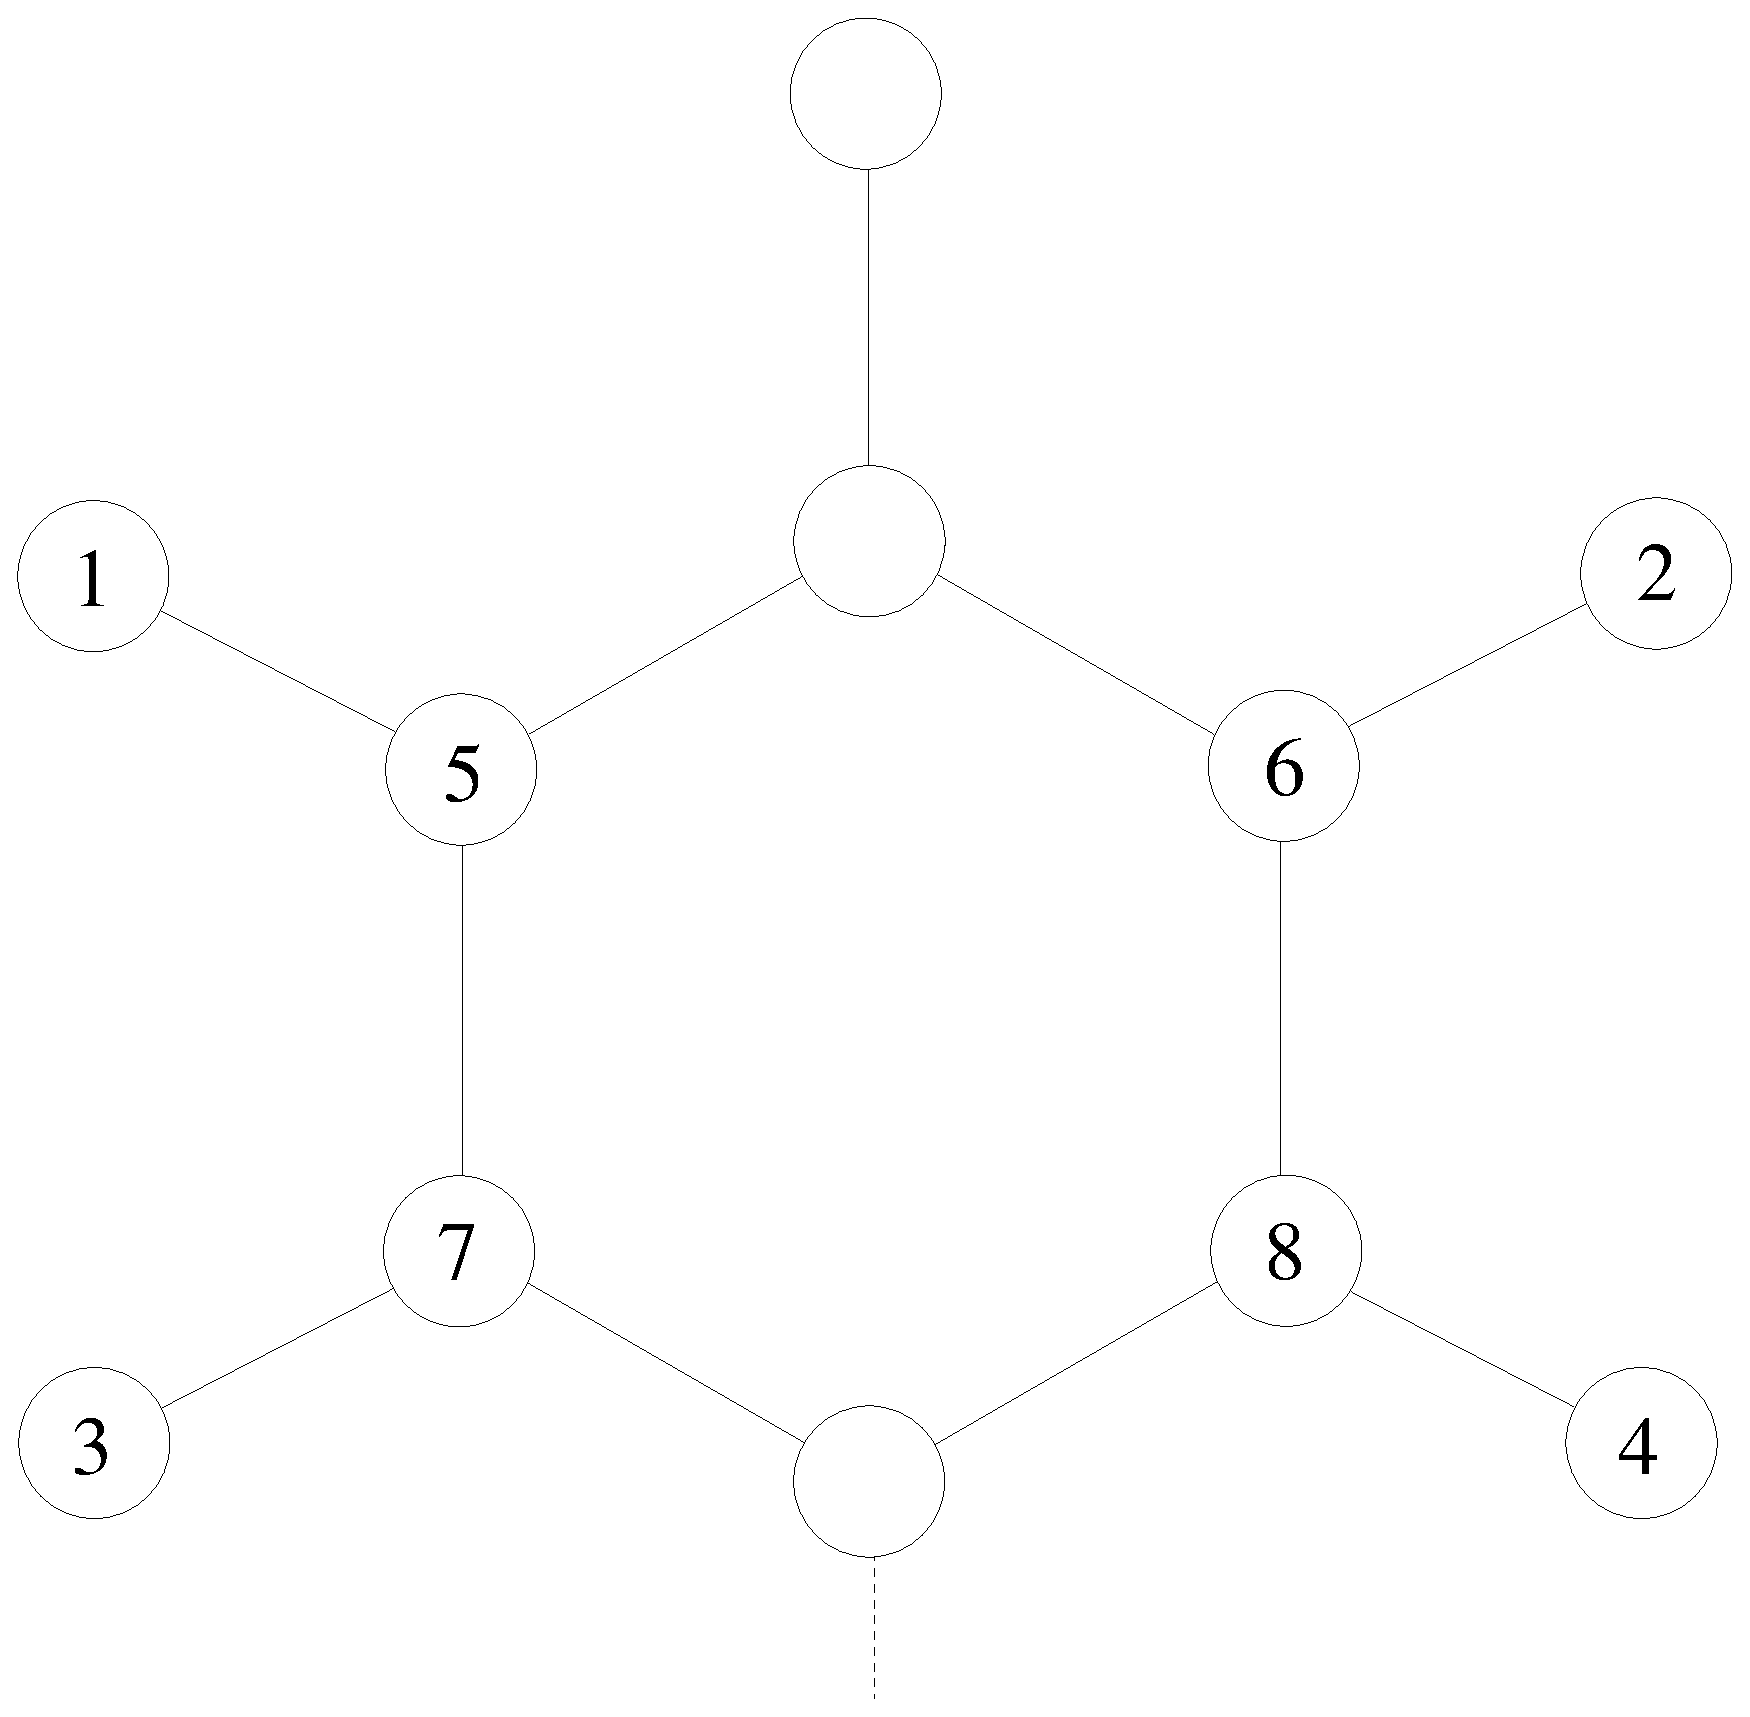
\includegraphics[width=0.5\textwidth]{PHE.eps}}
\end{figure}

For the phenylalanine example illustrated above we must allow three other pairs of
atoms to exchange if we swap 7 and 8. Hence a suitable {\tt perm.allow} entry is
{\obeylines
1
2 3
7 8 5 6 1 2 3 4
}
Here $n=2$ and $s=3$: if we exchange 7 and 8 then we must also exchange 5 and 6,
1 and 2, and 3 and 4. There are two atoms in each of the three secondary sets, 
since we have specified 7 and 8 as the two primary atoms.

Here is an example {\tt perm.allow} file for a water trimer using
the flexible {\keyw{QTIP4PF}\/} potential, where the energy is invariant to permutations
of water molecules and to exchanges of hydrogens in the same molecule. However,
hydrogens cannot exchange between different oxygens:
{\obeylines
4
3 2
1 4 7 2 3 5 6 8 9
2 0 
2 3
2 0 
5 6
2 0 
8 9
}
The first group of three oxygens has two atoms that must move with each oxygen,
i.e.~atoms 2 and 3 for oxygen 1, etc. Hydrogen permutations for each oxygen are
allowed by the three following groups. This scheme allows atoms to appear in more 
than one group. There must be a group containing each complete set of permutations
in order for permutation-inversion isomers to be recognised. The format
is compatible with an older scheme, where only pair swaps were allowed for
associated atoms, but now allows for more general permutations.

Scripts to generate allowed permutations automatically for CHARMM and AMBER are available from
the group web site. It is essential to use symmetrised versions of the corresponding
force fields! 

\ksec{PERMISOMER}{\/}: equivalent to {\keyw{PERMDIST}\/} above, expect that
distance minimisation 
with respect to permutational isomerisation is only carried out for stationary
points with energies that differ by less than the parameter specified by {\keyw{EDIFF}TOL}.
Hence permutational isomers should be identified, but the distance between minima with
different energies is not minimised with respect to atom permutations.
This option is provided for cases where the number of permutations is too 
minimise distances with respect to permutations in general.
Should be used with the {\keyw{PERMDIST}\/} keyword in {\tt OPTIM}.
The auxiliary file {\tt perm.allow} specifies which atoms may be permuted; see
{\keyw{PERMDIST}\/} above.
Note that the {\keyw{NATOMS}\/} keyword must precede {\it PERMISOMER\/} in the
{\tt pathdata} file.

\ksec{PERTURB}{ x\/}: initial maximum perturbation of the Cartesian coordinates of a minimum, 
when looking for a new connected minimum via a single-ended transition state search.

\ksec{PFOLD}{ n1 n2 x\/}: provides control parameters for the on-the-fly calculation
of committor probabilities during the construction of a stationary point database.
All new local minima are assigned an initial value of zero.
{\it n1} iterations are performed every {\it n2} cycles with parameter $\omega$ in
the successive overrelaxation equal to {\it x}.
Note that a valid solution also exists for all committor probabilities equal to unity.
I have seen the iteration converge to this solution for a  very small database that
has just been created with {\it DIJINIT\/}. 

\ksec{PLANCK}{ h\/}: specifies the value of Planck's constant in units of the
prevailing energy unit times seconds. This numerical value is required for 
regrouping free energies. For example, for the {\keyw{CHARMM}} potential $h$ needs
to be $9.546\times10^{-14}\,$s\,kcal/mol
See \S \ref{sec:units} for more details.


\ksec{PULL}{ \/}: add this keywork if the system has a non-zero static force 
added to the potential. {\tt PATHSAMPLE.2.1} only uses this keyword to determine the
number of zero Hessian eigenvalues (four). The attached atoms and force magnitude
are not required.

\ksec{PSCALE}{ x\/}: determines how the difference in committor probabilities,
$p$, is used to select the pair of minima used in the next attempted connection. If
$p/x > $ a random number drawn from $[0,1]$ then the distance criterion is accepted.
There is also a criterion for the minimum distance (see {\keyw{DSCALE}}).
If $p>x$ then the committor probability criterion is always satisfied; below $x$ the probability
of acceptance decreases linearly.

\subsection{R-Z}
\ksec{READMIN}{ file\/}: reads in the data for one or more minima from {\it file}
in {\tt OPTIM} min.data.info format and then stops. 
Any number of min.data.info files can be concatenated into {\it file}.
New entries will be created in {\tt min.data} and {\tt points.min}.
If {\tt min.A} and {\tt min.B} do not exist they are not created.
{\keyw{READMIN}} therefore provides an alternative way to start an initial
path calculation by providing minima, so long as {\tt min.A} and {\tt min.B}
are created by hand.
It also provides a way to add additional minima to an existing database, since
new entries should be appended. There is a check to make sure that the minima
added are different from all those currently known.

\ksec{REGROUP}{ x\/}: regroup the A and B sets using a disconnectivity graph 
analysis \cite{beckerk97,walesmw98,Wales03} at energy {\it x}. 
Any intervening minima that share a superbasin with an A or B minimum are reclassified
to belong to the A and B sets, respectively.\cite{TrygubenkoW06}
The number of minima and transition states {\it does not change}: only the
classification of minima as A or B is affected,
which will change any rate analysis that follows.
The corresponding
minima are printed in files {\tt min.A.regrouped} and {\tt min.B.regrouped}.

\ksec{REGROUPFREE}{ x\/}: the database will be regrouped by combining free
energy minima where forward and backward free energy barriers are both
less than {\it x}. Regrouping is performed iteratively until no further free
energy minima merge. 
In this scheme, groups that contain product and reactant minima
(A and B sets) are not allowed to merge. 
The regrouping continues even if product and reactant groups
could merge according to the barrier threshold: such mergers are simply forbidden.
Don't forget to assign an appropriate value for the Planck constant using the
{\keyw{PLANCK}\/} keyword. 
If one of the {\keyw{DIJKSTRA}}, {\keyw{SD}GT}, {\it SGT}, or {\it DGT} keywords is
present the corresponding analysis will be performed using the new groups
and free energies.

\ksec{REGROUPFREEAB}{ x\/}: the database will be regrouped as for
{\keyw{REGROUP}FREE\/} above, but only the A and B groups are changed.

\ksec{REGROUPPE}{ x\/}: the database will be regrouped based upon 
a superbasin analysis at potential energy $x$.
Minima will be reassigned as A and B-type if they are in a superbasin
with an A or B minimum for this threshold.
New files {\tt min.data.regrouped}, {\tt ts.data.regrouped}, {\tt min.A.regrouped}
and {\tt min.B.regrouped} will be created.
Don't forget to assign an appropriate value for the Planck constant using the
{\keyw{PLANCK}\/} keyword. See also {\keyw{REGROUP}RATE\/}.
{\keyw{REGROUP}PE\/} and {\keyw{REGROUP}RATE\/} are different from {\keyw{REGROUP}\/}
in that they actually change the internal database structure into free energy
minima and groups of transition states linking them.
In this scheme, groups that contain product and reactant minima
(A and B sets) are not allowed to merge. 
The regrouping continues even if product and reactant groups
could merge according to the barrier threshold: such mergers are simply forbidden.
If one of the {\keyw{DIJKSTRA}}, {\keyw{SD}GT}, {\it SGT}, or {\it DGT} keywords is
present the corresponding analysis will be performed using the new groups
and free energies.

\ksec{REGROUPRATE}{ x\/}: the database will be regrouped based upon harmonic transition
state theory rate constants. Minima are in the same group if they can interconvert
via a path that involves only rate constants greater than $x$.
Minima will be reassigned as A and B-type if they are in a group
with an A or B minimum for this threshold.
New files {\tt min.data.regrouped}, {\tt ts.data.regrouped}, {\tt min.A.regrouped}
and {\tt min.B.regrouped} will be created.
Don't forget to assign an appropriate value for the Planck constant using the
{\keyw{PLANCK}\/} keyword. See also {\keyw{REGROUP}PE\/}.
{\keyw{REGROUP}PE\/} and {\keyw{REGROUP}RATE\/} are different from {\keyw{REGROUP}\/}
in that they actually change the internal database structure into free energy
minima and groups of transition states linking them.
In this scheme, groups that contain product and reactant minima
(A and B sets) are not allowed to merge. 
The regrouping continues even if product and reactant groups
could merge according to the barrier threshold: such mergers are simply forbidden.
If one of the {\keyw{DIJKSTRA}}, {\keyw{SD}GT}, {\it SGT}, or {\it DGT} keywords is
present the corresponding analysis will be performed using the new groups
and free energies.

\ksec{REMOVESP}{\/}: the minima specified in files {\tt min.remove} and
{\tt ts.remove} are removed and new files {\tt min.data.removed},
{\tt ts.data.removed}, {\tt min.A.removed}, {\tt min.B.removed},
{\tt points.min.removed} and {\tt points.ts.removed}
are created with a consistent numbering scheme for the remaining stationary
points. The first lines of {\tt min.remove} and
{\tt ts.remove} must contain a single integer, which is the number of 
stationary points listed for removal on the remaining lines.

\ksec{RETAINSP}{\/}: minima {\bf not} specified in file {\tt min.retain} 
are removed and new files {\tt min.data.retained},
{\tt ts.data.retained}, {\tt min.A.retained}, {\tt min.B.retained},
{\tt points.min.retained} and {\tt points.ts.retained}
are created with a consistent numbering scheme for the remaining stationary
points. The first line of {\tt min.retain} 
must contain a single integer, which is the number of 
minima listed on the remaining lines.
Transition states are only retained if they link two minima specified in the
{\tt min.retain} file.

\ksec{REWEIGHT}{ nrwbins nrwreactant energyfile\/}: 
conditional probabilities of reactant minima are obtained from the quench
probabilities calculated using the energies in file {\tt energyfile}.
These energies could come from systematic quenching from an MD trajectory at
the same temperature, for example.
{\it nrwbins\/} is the number of bins to use in representing the quench
probability distribution and {\it nrwreactant} is the number of bins
to use in representing the minima in the reactant set.
This is a somewhat experimental option. Consult DJW before using!

\ksec{RIGIDBODIES}{ n\/}: specifies the number of rigid bodies; only one
of {\keyw{NATOMS}\/} and {\keyw{RIGIDBODIES}} should be present.

\ksec{SDGT}{ DisconnectSources AltPbb Rescale Normalise\/}: 
graph transformation rate calculation, which switches from sparse optimised to
dense optimised algorithms when the average number of connections
exceeds a certain threshold \cite{TrygubenkoW06}.
The four arguments are all logicals, so an example input line might look
\vbox{SDGT T T F F}. If true (the default) {\it DisconnectSources} specifies that
a full transformation should be performed for each source, disconnecting the 
other sources. The resulting rate constants correspond to the KMC result and
$k^{\rm KMC}$ \cite{Wales06}.
If {\it AltPbb\/} is true (default is false) then additional work is done to
maintain precision, which roughly doubles the execution time, but may be needed at low
temperature.
If {\it Rescale} is true (default false) an alternative strategy is used 
to try and prevent error propagation.
Setting {\it Normalise} true (default false) instructs {\tt GT2input.f90} to check the normalisation
of branch probabilities. This should not be necessary.

\ksec{SEED}{ n\/}: random number seed.

\ksec{SGT}{ DisconnectSources AltPbb Rescale Normalise\/}: 
sparse optimised graph transformation rate calculation \cite{TrygubenkoW06}.
The four arguments are all logicals, so an example input line might look
\vbox{SGT T T F F}. If true (the default) {\it DisconnectSources} specifies that
a full transformation should be performed for each source, disconnecting the 
other sources. The resulting rate constants correspond to the KMC result and
$k^{\rm KMC}$ \cite{Wales06}.
If {\it AltPbb\/} is true (default is false) then additional work is done to
maintain precision, which roughly doubles the execution time, but may be needed at low
temperature.
If {\it Rescale} is true (default false) an alternative strategy is used 
to try and prevent error propagation.
Setting {\it Normalise} true (default false) instructs {\tt GT2input.f90} to check the normalisation
of branch probabilities. This should not be necessary.

\ksec{SHORTCUT}{ minsep string\/}: try connecting minima that are further apart than {\it minsep\/}
steps on the best path, as calculated using Dijkstra's algorithm.
In the Dijkstra analysis minima with zero connections are removed. 
This value can be changed using a {\keyw{DIJKSTRA} n} line in {\tt pathdata}.
If the option argument {\it string\/} is set to {\it BARRIER\/} or {\it RATE\/} then
the strategy is different. We now look for pairs of minima on either side of
the highest barriers or minima linked by the smallest
rate constant on the best path, sorted according to the barrier height or the rate.
{\it minsep\/} is then used to define the largest number of steps away from 
the transition states for connection attempts.

\ksec{STARTFROMPATH}{ afile n1 n2 \/}: reads an initial path from file {\tt afile}. If this 
file is in {\keyw{DUMP}ALLPATHS} format then the keyword {\keyw{STAR}TTRIPLES} is also needed.
The files {\tt min.A} and {\tt min.B} are created: {\tt min.A} contains the entries
1 and {\it n1} and {\tt min.B} contains the entries 1 and {\it n2}.
If {\tt min.A} already exists then the run will terminate with a warning message
without overwriting it.

\ksec{STARTTRIPLES}{\/}: reads the initial path specified by
{\keyw{STAR}TFROMPATH a\/} from  file {\tt path.info.a} in the new {\keyw{DUMP}ALLPATHS}
format.

\ksec{SYSTEM}{ a\/}: the atom type label to be written to {\tt odata} files for {\tt OPTIM},
thus specifying the potential that {\tt OPTIM} will use.

\ksec{TAG}{ n x\/}: atom number {\it n\/} in the system is `tagged' by giving it 
an artificial mass {\it x\/}.

\ksec{TEMPERATURE}{ x\/}: specifies that the canonical ensemble at reduced temperature {\it x\/}
is to be used to calculate rate constants. Mutually exclusive with {\keyw{ENERGY}\/}.

\ksec{TRIPLES}{\/}: specifies that {\tt path.info} files read after startup 
have the new {\keyw{DUMP}ALLPATHS} format. Use {\keyw{STAR}TTRIPLES} and {\keyw{ADDTRIPLES}} to
read or add a single {\tt path.info} file in this format at the beginning of a run.

\ksec{TSTHRESH}{ x\/}: specifies that transition states above energy $x$ should
not be included in the database. Probably most useful with CHARMM, where genuine 
transition states with silly energies can certainly occur and give rise to underflow.

\ksec{TWOD}{\/}: the system is two-dimensional.

\ksec{UNRES}{\/}: specifies the UNRES potential.\cite{liwoopwrs97} % ,liwopwros97,liwokcgowrps98}

\ksec{UNTRAP}{ einc thresh\/}: try connecting minima to eliminate traps.
Connections are attempted between all minima and any of the minima in the
product set based on the largest barriers in the product direction, as estimated
from disconnectivity analysis at energy intervals of $einc$, starting from the
global minimum.
The product basin is defined as the set at the highest energy for which the 
minimum in question is not a member.
Candidate pairs of minima are sorted based upon the ratio of the
potential energy barrier to the potential energy difference between the minimum
in question and the lowest product minimum.
Hence this scheme is analogous to the {\keyw{FREEPAIRS}\/} procedure, but
uses individual minima and potential energy, instead of free energy.
Minima from the product basin above energy $thresh$ will only be considered if there
are no minima below this threshold.
In a second phase the original product minimum may be replaced by a minimum from
the same superbasin that is closer to the target minimum, so long as its energy
lies below the threshold.
Minima with zero connections are not considered; 
this value can be changed using a {\keyw{DIJKSTRA} n} line in {\tt pathdata}, even
though a Dijkstra analysis is not used.
See also the {\keyw{PAIRLIST}\/} keyword.
The {\keyw{UNTRAP} \/} keyword may provide the best way to remove artificial 
frustration from potential energy disconnectivity graphs.
It may be helpful to choose a larger value of {\it einc\/} than would be
used for the superbasin analysis in visualising the disconnectivity graph.
This will encourage connection attempts with minima of lower energy in the
expanded product superbasin. 

\ksec{USEPAIRS}{ Epathfile\/}: pairs of minima are chosen for connection attempts based
on the order of local minima specified in file {\tt Epathfile}, which must have the format
of a {\tt PATHSAMPLE} {\tt Epath} output file 9as generated by {\keyw{DIJKSTRA}\/}, etc.
This keyword is intended to follow a {\keyw{DUMMYTS}\/} run, where the stationary point
database has been refined using {\keyw{BHINTERP}\/} or {\keyw{BISECT}\/} runs in {\tt OPTIM}.
The dummy {\tt ts.data} and {\tt pairs.data} files must be renamed or removed
before the {\keyw{USEPAIRS}\/} run.
The pairs of minima are first chosen to be the adjacent structures from the list, then
second-neighbours, until all possible pairs have been tried.


\section{{\tt odata} files}
\label{sec:odatafiles}

The following {\tt odata} template
files may be necessary, one for each type of {\tt OPTIM} job which can be launched by {\tt PATHSAMPLE}.
If {\keyw{CONNECT}IONS} is set to one or fewer then only an {\tt odata.connect} template is
needed.
\smallskip
\begin{itemize}
\item {\tt odata.connect}: the template file for double-ended pathway searches.

\item {\tt odata.path}: template for pathway calculations to find the two minima connected by
steepest-descent paths to a single transition state. Reads in the eigenvector corresponding to
the negative eigenvalue (transition mode) from file {\tt vector.dump} produced by {\tt odata.tssearch}.

\item {\tt odata.tssearch}: performs a single-ended transition state search.

\end{itemize}

Please refer to the {\tt OPTIM} manual\cite{optim} for details of {\tt odata} files.
In the templates the {\tt odata} file should not contain any coordinates, and should terminate
with the {\it POINTS} or {\keyw{CHARMM}} keyword, as appropriate.
\pagebreak

\section{Output files}
\label{sec:output}

{\tt PATHSAMPLE} produces information about its progress on standard output;
more details can be obtained with the {\keyw{DEBUG}} keyword. 
The databases of minima and
transition states ({\tt min.data}, {\tt ts.data}, {\tt points.min} and {\tt points.ts}) described in
\S\ref{sec:input} are updated as necessary. 

\section{ A Note on Units and Planck's Constant}
\label{sec:units}

Aside from {\keyw{CHARMM}} and {\keyw{AMBER}} {\tt OPTIM} does no
unit conversions. These systems are treated differently, as explained below.
For all other cases {\tt PATHSAMPLE} is
expecting to receive $\ln\Pi_i \omega^2_i$ in the {\tt min.data}
and {\tt ts.data} files. {\tt PATHSAMPLE} converts $\omega$ to
$\nu$ using $\nu=\omega/2\pi$, but also does no unit conversions.
The rate constants are therefore in natural frequency units of
$\sqrt{\epsilon/m\sigma^2}$, where $\epsilon$ is the unit of energy,
$m$ is the unit of mass, and $\sigma$ is the unit of length.

For a system where all particles have equal masses, $m$, the rate constants
calculated by {\tt PATHSAMPLE} can therefore be converted to SI units
by multiplying by $\sqrt{(\epsilon/{\rm J})/(m/{\rm kg})(\sigma/{\rm m})^2}$.

For calculations involving free energy regrouping schemes we need to supply
a value for the Planck constant in reduced units via the {\keyw{PLANCK}} keyword.
Since the temperature is read in energy units, i.e.~$\epsilon$, so that $k_BT$
is in $\epsilon$, we need to define $h$ in reduced units so that terms like
$k_BT/h\nu$ are dimensionless. If $\nu$ is in reduced time units then we
need $(h/{\rm Js})$ divided by the unit of energy and the unit of time. 
The reduced value of $h$ is therefore
\begin{equation}
\frac{(h/{\rm Js})}{(\epsilon/{\rm J})
\sqrt{\displaystyle\frac{(m/{\rm kg})(\sigma/{\rm m})^2}{(\epsilon/{\rm J})}}} 
= \frac{(h/{\rm Js})}{\sqrt{(m/{\rm kg})(\sigma/{\rm m})^2(\epsilon/{\rm J})}}.
\end{equation}

For {\keyw{CHARMM}} and {\keyw{AMBER}} we need to diagonalise the reciprocal
mass-weighted Hessian in {\tt OPTIM}, where the various masses are known.
For convenience the frequency unit conversion is done in {\tt OPTIM} as
well, so that the rate constants calculated in {\tt PATHSAMPLE} are
in s$^{-1}$ and do not need to be converted.
The value required for the Planck constant is therefore different because
$\nu$ is not in reduced units. Instead, we need to convert $(h/{\rm Js})(\nu/{\rm s}^{-1})$
to kcal/mol, since these are the units of $k_BT$. Hence we need $(h/{\rm Js})/(\epsilon/{\rm J})$,
where $\epsilon$ is one kcal/mol. Since 1\,kcal/mol is $6.948\times10^{-21}\,$J
the required value for the {\keyw{PLANCK}\/} keyword in regrouping calculations
is $6.626\times10^{-34}/6.948\times10^{-21}=9.536\times10^{-14}$.


\section{Known Problems}
\label{sec:problems}

If all {\tt OPTIM} jobs are failing for some reason then it is likely
that the rsh command that starts the jobs on remote nodes will run out of
sockets. Using a single rsh command together with cp via nfs to copy results
back seems to have eliminated the previous problems that we sometimes saw
with socket errors.

Rate constant calculations with any graph transformation variant can be very
memory hungry. They will die with a segmentation fault if they run out
of memory.

%<examples>
\section{Example {\tt pathdata} files}
\label{sec:example}
\subsection{Starting from an {\tt OPTIM} {\tt path.info} file}

The following {\tt pathdata} file was used on a distributed memory machine.
It loads an initial path from {\tt path.info.startup} and creates {\tt min.A}
and {\tt min.B} files containing the entries 1 and 9 and 1 and 16, respectively.
1000 iterations of the committor probabilities are performed every cycle,
removing minima with one connection or fewer, and using a successive
overrelaxation parameter of 1.99.
Rate constants are calculated using graph transformation every 10 cycles,
again removing minima with one connection or fewer.
\medskip

\begin{table}[H]
\begin{center}
\begin{tabular}{ll}
JOBSPERNODE & 2 \\
NATOMS       &  56 \\
SYSTEM        & BL \\
STARTFROMPATH & startup 9 16 \\
COMMENT & ADDPATH add \\
GT & 1 10 \\
TEMPERATURE&    0.42 \\
DSCALE      &    3.0 \\
PSCALE       &   1.0 \\
PFOLD         &  1000 1 1.99 \\
CYCLES      &    500 \\
CONNECTIONS  &  1 \\
SEED      &     1 \\
PERTURB    &    0.3D0 \\
ETOL        &   0.0000005D0 \\
ITOL        &   0.1 \\
DIRECTION    &  AB \\
EXEC        &   /home/wales/bin/OPTIM.3.2 \\
TRIPLES & \\
STARTTRIPLES & 
\end{tabular}
\end{center}
\end{table}

\subsection{Starting from {\tt OPTIM} {\tt min.data.info} files}

It is also possible to start {\tt PATHSAMPLE} runs without an existing 
connection between the end points of interest. See keywords {\keyw{DIJINITSTART}\/}
and {\keyw{DIJINITCONT}\/}.
In this example we set up {\tt PATHSAMPLE} from {\tt min.data.info} files for the 
two minima and use {\keyw{DIJINITCONT}\/} to continue the run and seek an initial 
connection using {\tt PATHSAMPLE}.

First, a minimisation was run for each minimum using {\tt OPTIM} with the
{\keyw{DUMP}DATA} keyword set. The {\keyw{ENDHESS}} keyword was used to produce frequencies after a
{\keyw{BFGS}MIN\/} optimisation.
In a clean directory, with no preexisting {\tt PATHSAMPLE} files, two entries were created
in {\tt min.data} and {\tt points.min} using the {\tt PATHSAMPLE} {\keyw{READMIN}\/} keyword
to read each of the {\tt min.data.info} files in turn. {\tt min.A} and {\tt min.B} files were
then created using vi with one entry in each, pointing to minima 1 and 2, respectively. 
After creating a suitable {\tt odata.connect} file a single cycle of {\tt PATHSAMPLE}
was then run on one core to populate the database with enough minima to run on
multiple cores in subsequent connection attempts. Since there is only one possible connection
to try in the first cycle, it is necessary to use a single processor in this case
along with the {\keyw{DIJINITCONT}\/} keyword in {\tt pathdata}. A couple of cycles on
eight cores then produced a connection for this bulk BLJ$_{60}$ example.
\medskip

\begin{table}[H]
\begin{center}
\begin{tabular}{ll}
NATOMS   &      60 \\
COPYFILES & perm.allow \\
BULK  & 3.587037905 3.587037905 3.587037905 \\
PERMDIST \\
SYSTEM  &       LS \\
TEMPERATURE &   0.71 \\
CONNECTIONS &   1 \\
SEED        &   1 \\
PERTURB     &   0.40 \\
ETOL        &   1.0D-7  \\
ITOL        &   1.1D0 \\
GEOMDIFFTOL        &   0.1D0  \\
DIRECTION   &   AB \\
EXEC        &  /home/wales/bin/OPTIM \\
TRIPLES &  \\
ADDTRIPLES &  \\
STARTTRIPLES &  \\
 & \\
comment READMIN min.data.info.start \\
comment READMIN min.data.info.finish \\
comment CPUS 1 \\
 & \\
DIJINITCONT EXP \\
CYCLES        100 \\
JOBSPERNODE 1 \\
PAIRLIST 1
\end{tabular}
\end{center}
\end{table}
\medskip

The commented lines were used to read in the initial {\tt min.data.info} files.
A similar procedure can be used if an initial {\tt path.info} file is available
without a complete connection between the desired end points.

\chapter{DISCONNECT}

\section{DisconnectionDPS} 
\hypertarget{ddps}
\ddps is a program which purpose is to plot disconnectivity graphs \cite{beckerk97}.

It is adapted to read \ps data files.

Information and options are passed to the program in a file called {\tt dinfo}, which is keyword driven.

\subsection{Compulsory Keywords}

\ksec{DELTA}{dE}
Energetic separation of levels in basin analysis.

\ksec{FIRST}{E1}
Specifies the energy of the highest level on the energy axis.

\ksec{LEVELS}{n}
The number of levels at which to perform the basin analysis.

\ksec{MINIMA}{file}
Specifies filename for minima info.

\ksec{TS}{file}
Specifies filename for transition state info.

\subsection{Optional Keywords}

\ksec{CENTREGMIN}{}
If this keyword is present, then when a node splits into its daughter
nodes, the one containing the global minimum is always placed centrally
(even if other nodes carry more minima). This does not guarantee that
the global minimum is central in the overall diagram because other
nodes may push the one containing the global minimum over to one side.

\ksec{DUMPNUMBERS}{}
If present, a file called node\_numbers is written, listing the minima
associated with each node in each level. Nodes are listed from left to
right within each level.

\ksec{DUMPSIZES}{}
If present, a file called {\tt \verb|node_sizes|} is written, listing how many minima
are represented by each node in each level. Nodes are listed from left to
right in each level.

\ksec{EXCLUDEALL}{}
Removes all minima from the list of minima to be plotted.  This is to be
used in conjunction with the \keyw{PICK} command which can be used to specify
exclusively which minima are to be included.

\ksec{CONNECTMIN}{min}
If present then the analysis for a connected database is based upon minimum
number $min$. If absent then the global minimum is used to judge connectivity.

\ksec{COLOURPRINT}{}
For use with \keyw{TRMIN}, if present colour analysis written to node\_sections.   
Not actually required for colour analysis.

\ksec{IDENTIFY}{}
If present, the branch ends are labelled with the lowest-energy minimum
they represent.

\ksec{IDENTIFY\_NODE}{max\_min}
If present, the nodes are labelled with the format \verb|N1_N2|, where N1 is the number of level,
N2 is the number of the node at that level. The label is only printed if the
number of minima below that node is smaller than \verb|max_min|. With this info
you can pick the number of minima corresponding to that node from the {\tt \verb|node_numbers|} file,
produced by using the keyword \keyw{DUMPNUMBERS}... (and then print any branch of the graph separately)

\ksec{IDENTIFY\_NODE\_SIZE}{max\_min2}
If present, the nodes are labelled with number of minima corresponding to that node. 
The label is only printed if the number of minima below that node is smaller than max\_min2

\ksec{IDMIN}{min}
Label this minimum on the graph. Repeat to label more than one minimum.

\ksec{LABELFORMAT}{fmt}
Specifies the Fortran format string for the energy level labels. The default
is F6.1.

\ksec{LABELSIZE}{n}
Set the size of the fonts in case of the labels (for \keyw{IDENTIFY}, \keyw{IDENTIFY\_NODE} ...)
Default is 10 pt.

\ksec{LETTER}{}
If present, the graph is formatted for American letter paper rather than
European A4.

\ksec{LOWEST}{n}
If present, only the branches leading to the lowest $n$ minima are drawn. The
pruning occurs after the basin analysis, so the "discarded" minima can still
influence the connectivities.

\ksec{MONOTONIC}{}
If present, all minima not lying at the bottom of a monotonic sequences are
not drawn. This tends to reduce the number of branches drastically. If the
keyword \keyw{LOWEST} is also used, the MONOTONIC sequence analysis is applied after
the high energy minima have been discarded.

\ksec{NCONNMIN}{} Minima with NCONNMIN connections or fewer are discarded. Default is zero.

\ksec{NOBARRIERS}{}
If present, all transition state energies are reset to the energy of the higher
of the two minima they connect. This transforms the energy landscape to the
type explored by gmin.

\ksec{PICK}{file}
Specifies the name of a list of numbers of minima, one per line.  Minima on
this list are included on the graph.  Minima preceded with a minus sign are
removed from the graph.  This process is executed after the commands
\keyw{MONOTONIC}, \keyw{LOWEST} and \keyw{EXCLUDEALL} have been executed, thereby making it
possible to override them for particular minima.  Examples: 
\begin{itemize}
\item 1. To remove certain minima from a full plot, just specify PICK 
and a list of negative minima numbers.
\item 2. To include only specific minima, use \keyw{EXCLUDEALL} and
\keyw{PICK} plus a list of positive minima numbers.  All basin analysis includes
the full sample and is performed before minima are removed or added back in.
\end{itemize}

\ksec{NOSPLIT}{}
By default, every minimum is indicated by its own branch, which splits off
from the parent basin even if the minimum and its lowest transition state do
not straddle an energy level in the basin analysis. This is to avoid it being
dependent on precisely where the levels are placed (bulk shifting of the levels
would cause some branch ends to appear or disappear rather than change node
if this were not the case). The \keyw{NOSPLIT} option turns this feature off, so that
if two minima are separated by a barrier lower than the level above their own
energy, they are grouped together. This option should probably never be used.

\ksec{TRMIN}{n max file file ...}
Label $n$ different sections of the graph in colour as specified by the 
minima in each file, one file for each section.  
Each file is a list of numbers of minima, 
one per line as for \keyw{PICK}. $max$ is the total number of minima, not the number 
in the colour files. 
currently used for array allocation.
Colours are chosen automatically to spread over a rainbow spectrum  
(from red to purple) in the order the files are specified but colours can 
be specified individually at both COLOURMARKER in this file. - vkd 

\keyw{TSTHRESH}{threshold} ignore transition states above this threshold.
\keyw{MAXTSENERGY}{threshold} ignore transition states above this threshold.
\keyw{MAXTSBARRIER}{threshold} ignore transition states with both barriers above this threshold.

\keyw{WEIGHTS}{file}

If present, use weights in $file$ to scale the horizontal width. The expected 
format of $file$ is:
bin number  Vmin   Vmax  ln weight

\section{Manipulate}
\hypertarget{manipulate}
\dman is a program for editing disconnectivity graphs produced by \hyperlink{ddps}{\ddps}.
 The user types in commands on the terminal, and the postscript file is
 rewritten after each command.  [Commands are not case sensitive.]

 To get started, make a tree.ps file with \ddps.  Run \prog{ghostview}
 in the background, and start \prog{manipulate}.  Type "READ" to load the graph.
 Now use the coordinates of the mouse pointer in ghostview to identify the
 approximate coordinates $x$ and $y$ of the node you would like to move. \progl{manipulate}
 will find the closest node to the point you specify and can perform the
 following operations.  Nodes are only moved horizontally.

\subsection{Commands}
\ksec{ALIGN}{x y}
Align the node vertically with its parent in the next level up.

\ksec{JOINUP}{x y}
Removes the parent of a node and connects the node to its grandparent
instead.  Only useful for nodes with no sisters.

\ksec{MOVEBY}{x y dx}
Moves the node by a horizontal amount $dx$.

\ksec{MOVETO}{x y x'}
Moves the node to horizontal coordinate $x'$.

\ksec{PIVOT}{x y x' y'}
Moves the $x$ coordinate of a node to $x'$ and pivots all lines connected
below about their intersection with the line $y = y'$. The value of $y'$
should be specified precisely as one of the levels of the graph.

\ksec{PSQUEEZE}{x y f}
Recursively compresses all nodes below the one specified by a fixed
factor $f$ about the $x$ coordinate of the node.

\ksec{QUIT}{} Leave the program

\ksec{RALIGN}{x y}
Recursive align.  Same as \keyw{ALIGN} but translates all nodes connected below
the one moved by the same amount.

\ksec{RMOVEBY}{x y dx}
Recursive moveby.  Same as \keyw{MOVEBY} but translates all nodes connected below
by the same amount.

\ksec{RMOVETO}{x y x'}
Recursive moveto.  Same as \keyw{MOVETO} but translates all nodes below by the
same amount.

\ksec{RSQUEEZE}{x0 x1 y f}
Scales all $x$ coordinates in the range $x0$ to $x1$ on the level at $y$ about the
midpoint of the range by a factor $f$, and recursively translates nodes below
by the same amount.

\ksec{SQUEEZE}{x0 x1 y f}
Same as \keyw{RSQUEEZE} but does not recursively translate the nodes below.

\ksec{UNDO}{} Undoes the last command by reading the previous state from disk.
\ksec{UPALIGN}{x y} Vertically aligns the parent of the specified node.





\clearpage
\phantomsection
\pdfbookmark[0]{Titlepage}{title} % Sets a PDF bookmark for the title page
\maketitle

\clearpage
\phantomsection
\pdfbookmark[0]{\contentsname}{contents} % Sets a PDF bookmark for the Table of Contents
\tableofcontents

\clearpage
\phantomsection
\pdfbookmark[0]{List of Figures}{lof} % Sets a PDF bookmark for the List of Figures
\listoffigures

\clearpage
\phantomsection
\pdfbookmark[0]{List of Tables}{lot} % Sets a PDF bookmark for the List of Tables
\listoftables

%\clearpage
%\phantomsection
%\pdfbookmark[0]{List of Algorithms}{loa} % Sets a PDF bookmark for the List of Tables
%\listof{algorithm}{List of Algorithms}


\clearpage
\phantomsection
\pdfbookmark[0]{List of Algorithms}{loa} % Sets a PDF bookmark for the List of Tables
\listof{algorithm}{List of Algorithms}

\cleardoublepage
\phantomsection
\addcontentsline{toc}{chapter}{Bibliography}

\def\aciee{Angew.~Chem.~Int.~Ed.~Engl.}
\def\acp{Adv.~Chem.~Phys.}
\def\acr{Acc.~Chem.~Res.}
\def\ac{Acta.~Crystallogr.}
\def\ajp{Am.~J.~Phys.}
\def\am{Adv.~Mater.}
\def\apl{Appl.~Phys.~Lett.}
\def\ap{Ann.~Physik}
\def\Pa{Physica A}
\def\arpc{Ann.~Rev.~Phys.~Chem.}
\def\bbpc{Ber. Bunsenges. Phys. Chem.}
\def\bc{Biochemistry}
\def\cccc{Coll.~Czech.~Chem.~Comm.}
\def\cj{Comput.~J.}
\def\cpc{Comp.~Phys.~Comm.}
\def\cpl{Chem.~Phys.~Lett.}
\def\cp{Chem.~Phys.}
\def\crev{Chem.~Rev.}
\def\dalton{J.~Chem.~Soc., Dalton Trans.}
\def\el{Europhys.~Lett.}
\def\faraday{J.~Chem.~Soc., Faraday Trans.}
\def\fartrans{J.~Chem.~Soc., Faraday Trans.}
\def\fdisc{J.~Chem.~Soc., Faraday Discuss.}
\def\ic{Inorg.~Chem.}
\def\ijmpc{Int.~J.~Mod.~Phys.~C}
\def\ijqc{Int.~J.~Quant.~Chem.}
\def\jacers{J. Am. Ceram. Soc.}
\def\jacs{J.~Am.~Chem.~Soc.}
\def\jap{J.~Appl.~Phys.}
\def\jas{J.~Atmos.~Sci.}
\def\jcc{J.~Comp.~Chem.}
\def\jce{J.~Chem.~Ed.}
\def\jcis{J.~Colloid Interface Sci.}
\def\jcp{J.~Chem.~Phys.}
\def\jcscc{J.~Chem.~Soc., Chem.~Commun.}
\def\jcsft{J.~Chem.~Soc., Faraday Trans.}
\def\jetp{J.~Exp.~Theor.~Phys.~(Russia)}
\def\jmc{J.~Math.~Chem.}
\def\jmsp{J.~Mol.~Spec.}
\def\jmst{J.~Mol.~Structure}
\def\jncs{J.~Non-Cryst.~Solids}
\def\jpa{J.~Phys.~A}
\def\jphysc{J.~Phys.~C}
\def\jpca{J.~Phys.~Chem.~A}
\def\jpcb{J.~Phys.~Chem.~B}
\def\jpcm{J.~Phys.~Condensed Matter.}
\def\jpcssp{J.~Phys.~C: Solid State Phys.}
\def\jpcs{J.~Phys.~Chem.~Solids.}
\def\jpc{J.~Phys.~Chem.}
\def\jpfmp{J.~Phys.~F, Metal Phys.}
\def\jpsj{J.~Phys.~Soc.~Jpn.}
\def\jsp{J.~Stat.~Phys.}
\def\mg{Math.~Gazette}
\def\molphys{Mol.~Phys.}
\def\molp{Mol. Phys.}
\def\mrsb{Mater.~Res.~Soc.~Bull.}
\def\msr{Mater.~Sci.~Rep.}
\def\nat{Nature}
\def\njc{New J.~Chem.}
\def\pac{Pure.~Appl.~Chem.}
\def\phys{Physics}
\def\pla{Phys.~Lett.~A}
\def\phm{Philos. Mag.}
\def\pma{Philos.~Mag.~A}
\def\pmb{Philos.~Mag.~B}
\def\pml{Philos.~Mag.~Lett.}
\def\pnasu{Proc.~Natl.~Acad.~Sci.~USA}
\def\pnas{Proc.\ Natl.\ Acad.\ Sci.\  USA}
\def\pra{Phys.~Rev.~A}
\def\prbcm{Phys.~Rev.~B}
\def\prb{Phys.~Rev.~B}
\def\prc{Phys.~Rev.~C}
\def\prd{Phys.~Rev.~D}
\def\prep{Phys.~Reports}
\def\pre{Phys.~Rev.~E}
\def\prl{Phys.~Rev.~Lett.}
\def\prsa{Proc.~R.~Soc.~A}
\def\pr{Phys.~Rev.}
\def\psfg{Proteins: Struct., Func.~and Gen.}
\def\pssb{Phys.~State Solidi B}
\def\pss{Phys.~State Solidi}
\def\rmp{Rev.~Mod.~Phys.}
\def\rpp{Rep.~Prog.~Phys.}
\def\sci{Science}
\def\ss{Surf.~Sci.}
\def\tca{Theor.~Chim.~Acta}
\def\tetra{Tetrahedron}
\def\zfpd{Z.~Phys.~D}
\def\zpb{Z.~Phys.~B.}
\def\zpc{Z.~Phys.~Chem.}
\def\zpdamc{Z.~Phys.~D}
\def\zpd{Z.~Phys.~D}

%\bibliographystyle{thesis}
\bibliographystyle{apalike}
\bibliography{wgdoc}
\bibliography{repdoc}

\end{document}

